\documentclass[tcc,capa,table]{textsi}

%\usepackage[brazilian]{babel} % Linguagem do documento: Português-brasileiro
\usepackage[utf8]{inputenc} % Codificação do arquivo .tex. IMPORTANTE: O arquivo deve ser salvo utilizando a codificação UTF-8 para mostrar corretamente os caracteres!
\usepackage[T1]{fontenc} % Permite que se faça cópia do texto do PDF de maneira correta, usando a codificação de fonte T1

% Alguns pacotes disponíveis no latex para adição e manipulação de elementos do documento
\usepackage{array,booktabs}
\usepackage{enumitem}
\usepackage{listings}

\usepackage{makecell}
\usepackage{graphicx,subfigure}
\usepackage{multirow}
\usepackage{xcolor}
\usepackage{pdfpages}
\usepackage{lipsum}
\usepackage{longtable}
\usepackage{placeins}
\usepackage{float}
\usepackage{xcolor}
\usepackage{booktabs}
\usepackage{tabularx}
\graphicspath{{images/}}

\lstset{
  basicstyle=\ttfamily\footnotesize,
  breaklines=true,
  frame=single,
  columns=fullflexible,
}

% Título do trabalho
\title{Nexo --- aplicativo de monitoramento do humor para pessoas com transtorno bipolar}

% Autor do trabalho. Primeiro argumento: Último sobrenome; Segundo argumento: Restante do nome
\author{Porcellis}{Pedro Lucas}

% Orientador do trabalho. Primeiro argumento (opcional): titulação do orientador. Segundo argumento (obrigatório): Último sobrenome; Terceiro argumento (obrigatório): Restante do nome
\advisor[Prof.~Me.]{Nunes}{Flávio}

% Instituição do orientador do trabalho.
\instituicaoadvisor{IFSul}

% Descomente a linha abaixo se tens co-orientador. Segue o mesmo formato do orientador do trabalho.
%\coadvisor[Prof.~Dr.]{Aguiar}{Marilton Sanchotene de}

% Descomente a linha abaixo se tens colaborador. Segue o mesmo formato do orientador do trabalho.
%\collaborator[Prof.~Dr.]{Aguiar}{Marilton Sanchotene de}

% Membro 1 da banca. Um argumento único, contendo titulação e nome completo.
\membroi{Prof.~Dr. Fulano de Souza e Silva}
% Instituição do membro 1 da banca.
\instituicaomembroi{UFI}

% Membro 2 da banca. Segue o mesmo formato que o membro 1.
\membroii{Prof. Dr. Sicrano Silveira Rosa}
% Instituição do membro 2 da banca.
\instituicaomembroii{UFPG}

% Descomente se tens um terceiro membro na banca. Membro 3 da banca. Segue o mesmo formato que o membro 1.
\membroiii{Prof. Dr. Beltrano Pereira Tavares}
% Descomente se tens um terceiro membro na banca. Instituição do membro 3 da banca.
\instituicaomembroiii{UFCR}

% Palavras-chave do trabalho desenvolvido.
\keyword{Ecological Momentary Assessment}
\keyword{Transtorno Bipolar}
\keyword{Monitoramento de humor}
\keyword{React Native}
\keyword{TypeScript}
\keyword{PostgreSQL}

% XXX: Fix longtables not having a prefix. Fucking POS template; shoulda stick
% to rawdogging ABNT2 or just use the IFRJ one which is actually complete

\makeatletter
\def\LT@c@ption#1[#2]#3{%
  \LT@makecaption#1\fnum@table{#3}%
  \def\@tempa{#2}%
  \ifx\@tempa\@empty\else
    \addcontentsline{lot}{table}%
      {\protect\numberline{\fnum@table}{\ignorespaces #2}}%
  \fi}
\makeatother


% Links internos do PDF (sumário, referências cruzadas, citações) clicáveis,
% mas sem cor e sem moldura -- discretos, ao invés do estilo "link de HTML".
% Deve ser o último pacote carregado no preâmbulo.
\usepackage[hidelinks,bookmarksnumbered]{hyperref}


\begin{document}

% Descomente se você tem orientadora, e não orientador.
%\renewcommand{\advisorname}{\orientadora}

% Descomente se você tem coorientadora, e não orientador.
%\renewcommand{\coadvisorname}{\coorientadora}

% Faz com que o título apareça
\maketitle

\sloppy

% Ficha catalográfica e folha de aprovação
\fichacatalografica
\folhadeaprovacao

%Opcional - dedicatória
\begin{dedicatoria}
	Texto da Dedicatória
\end{dedicatoria}

%Opcional - agradecimentos
\begin{agradecimentos}
	Texto dos Agradecimentos
\end{agradecimentos}

%Opcional - epígrafe
\begin{epigrafe}
	``Texto da Epígrafe'' \\
	Autor da Epígrafe
\end{epigrafe}

% Resumo em língua vernácula (a que você está escrevendo o documento)
\begin{abstract}
\noindent
Este trabalho apresenta o desenvolvimento do Nexo, uma aplicação móvel de
código aberto voltada ao monitoramento do humor de pessoas com Transtorno
Bipolar, fundamentada nos princípios da \textit{Ecological Momentary
Assessment} (EMA). O objetivo foi conceber uma ferramenta que integrasse, em
uma única plataforma, o registro de humor, a qualidade do sono, gatilhos e
ações de cuidado, de modo a auxiliar o usuário na identificação de padrões
afetivos ao longo do tempo. A pesquisa caracteriza-se como aplicada, de
natureza exploratória, e combinou levantamento bibliográfico, aplicação de
questionário com potenciais usuários e análise de aplicativos similares,
empregando o modelo incremental e princípios ágeis com \textit{Kanban} no
desenvolvimento. Como resultado, obteve-se um protótipo funcional composto por
uma API REST e um aplicativo móvel, ambos em TypeScript, com processamento de
indicadores em segundo plano, implantação automatizada e testes automatizados
da API.
Conclui-se que os objetivos propostos foram alcançados, evidenciando a
viabilidade de uma solução de autorregistro alinhada à privacidade e à
autonomia do usuário sobre seus dados.
\end{abstract}

% Resumo em língua estrangeira
\begin{englishabstract}%
  {Ecological Momentary Assessment, Bipolar Disorder, Mood Tracker, React
  Native, TypeScript, PostgreSQL}

  \noindent
  This work presents the development of Nexo, an open-source mobile application
  for mood monitoring aimed at people with Bipolar Disorder, grounded in the
  principles of the Ecological Momentary Assessment (EMA). The goal was to
  design a tool that integrated, within a single platform, the recording of
  mood, sleep quality, triggers, and care actions, in order to help users
  identify affective patterns over time. The research is applied and
  exploratory in nature, combining a literature review, a questionnaire applied
  to potential users, and an analysis of similar applications, while adopting
  an incremental development model and agile principles with Kanban. As a
  result, a functional prototype was produced, composed of a REST API and a
  mobile application, both written in TypeScript, with background processing of
  indicators, automated deployment, and automated tests for the API. It is
  concluded that the proposed objectives were achieved, demonstrating the
  feasibility of a self-tracking solution aligned with user privacy and
  autonomy over their data.
\end{englishabstract}

%Lista de Figuras
\listoffigures

%Lista de Tabelas
\listoftables

% Lista de códigos
\lstlistoflistings

%lista de abreviaturas e siglas
\begin{listofabbrv}{REST} % <- Insira aqui a maior sigla da sua lista de siglas.
	% O conteúdo dentro dos colchetes é a sigla, e o texto ao lado é o seu significado
	\item[TAB] Transtorno Afetivo Bipolar
  \item[BAP] Bipolar Affective Disorder
  \item[TCC] Terapia Cognitivo-comportamental
  \item[EMA] \textit{Ecological Momentary Assessment}
  \item[UML] \textit{Unified Modeling Language}
  \item[DAO] \textit{Data Access Object}
  \item[REST] \textit{Representational State Transfer}
  \item[API] \textit{Application Programming Interface}
  \item[UX] \textit{User Experience}
  \item[SSH] \textit{Secure Shell}
  \item[CI] \textit{Continuous Integration}
  \item[CD] \textit{Continuous Deployment}
\end{listofabbrv}

%Sumario
\tableofcontents

% Chapter é a seção primária do documento. Toda vez que é chamado este comando, uma quebra de página é adicionada;
\chapter{Introdução}

O avanço da tecnologia digital tem transformado profundamente a forma como
indivíduos interagem com sua saúde mental, com seus hábitos cotidianos e com os
recursos disponíveis para o autocuidado. Em um cenário de sobrecarga de
informações e de crescimento dos quadros de ansiedade e depressão, cresce
também a busca por ferramentas que auxiliem no reconhecimento e na gestão das
emoções de forma autônoma e personalizada.

Esse cenário é particularmente relevante para o Transtorno Afetivo Bipolar
(TAB), condição caracterizada por flutuações cíclicas do humor que tornam
difícil, para o próprio indivíduo, identificar em que etapa do ciclo se
encontra. O autorregistro contínuo --- aproximando a coleta do momento em que a
experiência ocorre, nos moldes do \textit{Ecological Momentary Assessment} ---
é uma via consolidada para reduzir os vieses de memória e favorecer o
desenvolvimento de consciência afetiva e de autoconhecimento.

No entanto, as aplicações disponíveis para esse fim ainda apresentam lacunas:
frequentemente fragmentam sono, humor, gatilhos e ações de cuidado em telas
isoladas, restringem a exportação dos dados e operam como soluções fechadas,
com pouca transparência sobre o tratamento das informações sensíveis que
coletam. Essas limitações evidenciam a necessidade de uma solução que concentre
os registros e preserve a autonomia do usuário sobre os próprios dados.

Diante dessas lacunas, este trabalho tem como objetivo desenvolver o Nexo, uma
aplicação móvel de código aberto voltada ao acompanhamento do humor de pessoas
com TAB, capaz de produzir indicadores que auxiliem o usuário na percepção de
padrões afetivos ao longo do tempo. Para construí-la, o desenvolvimento
apoia-se em levantamento bibliográfico, na aplicação de um questionário a
potenciais usuários e na análise de aplicativos similares para levantar
requisitos, e culmina na modelagem, na implementação e na verificação
automatizada do sistema.

Além desta introdução, o documento está organizado em oito capítulos. O
Capítulo 2 revisa a literatura sobre transtorno bipolar, autorregistro e
\textit{Ecological Momentary Assessment}, situando as limitações dos
aplicativos existentes. O Capítulo 3 apresenta as metodologias de
desenvolvimento e de pesquisa adotadas, incluindo o questionário aplicado e a
análise de aplicativos similares. O Capítulo 4 descreve o Nexo, seus requisitos
e a modelagem do sistema. O Capítulo 5 trata do design visual e da estrutura de
navegação. O Capítulo 6 apresenta as tecnologias empregadas. O Capítulo 7
descreve a arquitetura e o funcionamento das principais funcionalidades. O
Capítulo 8 discute a estratégia de verificação adotada. Por fim, o Capítulo 9
apresenta as considerações finais e as melhorias futuras.

\chapter{Saúde e autocuidado mental no mundo digital}

% TODO: Move these refs into bibtex

No quesito de saúde mental, a bipolaridade ou pelo seu nome científico,
Transtorno Afetivo Bipolar (TAB), é uma das doenças mentais mais comuns e
responsável por uma gama muito grande de disfunções mentais. De acordo com
o estudo conduzido por \citet{Merikangas2011}, no âmbito do World Mental
Health Survey Initiative da Organização Mundial da Saúde, com mais de 61 mil
adultos entrevistados em 11 países, a prevalência ao longo da vida do espectro
bipolar é de 2,4\% da população mundial, e a prevalência em um período de 12
meses é de 1,5\%. No contexto do Brasil, segundo a Associação Brasileira de
Transtorno Bipolar (ABTB), capítulo brasileiro da \textit{International Society for
Bipolar Disorders} (ISBD) \citep{abtb}, a bipolaridade afeta cerca de
4\% da população, o que representaria uns 7,6 milhões de
pessoas. Esse número, embora soe pouco expressivo, levando em consideração o
contingente de pessoas no país, é preocupante, dado o fato de que a
bipolaridade é (1) complexa de se detectar e (2) muitas vezes, acaba passando
despercebida ou enquadrada dentro de um quadro de depressão unipolar
(depressão).

Embora o autorregistro seja amplamente recomendado no acompanhamento
de pessoas com TAB, dado seu potencial de validade clínica e de efeito
sobre desfechos relevantes~\cite{Faurholt:2016}, sua realização de
maneira contínua representa um desafio.
Em muitos casos, o paciente depende da própria memória para reconstruir
retrospectivamente seu estado emocional, a qualidade do sono,
acontecimentos cotidianos e outros fatores que podem ter influenciado
seu humor. Esse processo está sujeito, naturalmente, a vieses de
recordação e dificulta a identificação de padrões temporais, especialmente
quando as informações são coletadas apenas durante consultas clínicas.

Nesse contexto, o \textit{Ecological Momentary Assessment} (EMA)
consolidou-se como uma importante abordagem metodológica para coleta
de dados em saúde mental. Diferentemente de avaliações retrospectivas,
o EMA propõe que informações sejam registradas no ambiente natural do
indivíduo e próximas ao momento em que as experiências ocorrem, reduzindo
vieses de memória e permitindo observar a dinâmica dos estados afetivos
ao longo do tempo \citep{EbnerPriemer2009}. Além de proporcionar maior
validade ecológica aos dados coletados, essa estratégia tem sido
empregada em diversas áreas da pesquisa comportamental, incluindo
transtornos do humor \citep{Collins2003, EbnerPriemer2009}, permitindo
compreender a relação entre fatores contextuais, eventos cotidianos e
alterações do humor.

Nesse contexto, o uso de tecnologias digitais tem se mostrado uma via
promissora para sistematizar esse tipo de acompanhamento. Pesquisas indicam
que pessoas com transtornos do espectro bipolar demonstram alta adesão ao
monitoramento emocional quando este é feito de forma acessível, visual e
integrada ao seu cotidiano, com estudos reportando taxas de conclusão acima
de 90\% em protocolos de avaliação momentânea
via \textit{smartphone} \citep{Ryan2020} \footnote{
  Vale citar porém, que esse artigo tem limitações de generalização:
  os resultados são limitados a um grupo de pessoas que possuiam um maior
  contato com tecnologia.
}.

Entre as formas mais comuns de implementação do EMA encontra-se o
autorregistro contínuo (\textit{journaling}), no qual o indivíduo
registra sistematicamente aspectos relevantes do cotidiano, como
humor, qualidade do sono, eventos significativos, sintomas percebidos
e outras informações contextuais. Com o acúmulo desses registros,
torna-se possível identificar padrões de comportamento, reconhecer fatores
associados às alterações de humor e favorecer o desenvolvimento da
autoconsciência sobre a própria condição, constituindo uma ferramenta
complementar ao processo de autoconhecimento e autogestão do
comportamento \citep{Melton2013}.

A ampla disseminação dos dispositivos móveis ampliou significativamente
as possibilidades de utilização dessas estratégias fora do ambiente
clínico. Smartphones acompanham o indivíduo durante praticamente toda
sua rotina, permitindo que registros sejam realizados no momento em que
as experiências ocorrem e reduzindo o esforço necessário para manutenção
do acompanhamento contínuo. Como consequência, diversas aplicações
voltadas ao monitoramento da saúde mental passaram a incorporar princípios
do EMA em seus fluxos de utilização, oferecendo registros estruturados
e visualizações históricas capazes de auxiliar usuários e profissionais
de saúde \citep{Faurholt:2016}.

Apesar da crescente disponibilidade de aplicações voltadas ao acompanhamento
do humor, estudos recentes que avaliaram especificamente os aplicativos mais
utilizados por pessoas com TAB para monitoramento de humor e sono apontam
limitações importantes quanto à integração entre esses domínios, ao controle
do usuário sobre seus próprios dados e à acessibilidade das políticas de
privacidade, muitas vezes redigidas em nível de leitura incompatível com o
público geral \citep{Morton2022}.

Em paralelo, análises mais amplas do ecossistema de aplicativos de
saúde mental também identificam riscos recorrentes de privacidade,
como permissões desnecessárias e vazamento de dados sensíveis \citep{Iwaya:22}.
Essas limitações evidenciam a necessidade de soluções que conciliem
boas práticas de engenharia de software, proteção de dados pessoais e
recursos que apoiem a identificação de padrões emocionais ao longo do tempo.

Diante desse contexto, este trabalho propõe o desenvolvimento de uma
aplicação móvel fundamentada nos princípios do
\textit{Ecological Momentary Assessment} voltada ao acompanhamento
cotidiano de pessoas com Transtorno Afetivo Bipolar. O sistema busca
integrar registros estruturados de humor, qualidade do sono, gatilhos
e ações de cuidado em uma única plataforma, produzindo indicadores que
auxiliem o usuário na visualização de padrões e no desenvolvimento da
consciência sobre seu próprio estado afetivo. Ressalta-se que a aplicação
não possui finalidade diagnóstica nem substitui o acompanhamento realizado
por profissionais de saúde, sendo concebida como uma ferramenta de apoio
ao autorregistro e ao autocuidado.

\chapter{Metodologias}
\label{chapter:methodologies}

Como primeiro passo, para conseguir viabilizar construir um \textit{software}
com qualidade, é necessário adotar metodologias que fundamentam a ideia e o
embasem o processo. De tal sorte que, ajudem a levantar quais requisitos esse
\textit{software} deve atender, priorizar funcionalidades, quebrar o escopo em
entregáveis que possam ser validados, e desenvolver os mesmos de forma
sustentável. Esse capítulo se debruça, tanto na abordagem da metodologia de
pesquisa do projeto, quanto também detalha o método de desenvolvimento de
\textit{software} escolhido.

\section{Metodologia de Desenvolvimento de \textit{software}}

Existem diversas abordagens para o desenvolvimento de \textit{software}, cada
uma com seus respectivos prós e contras. Todos procuram responder a uma mesma
necessidade: dar forma ao processo de desenvolvimento, para que ele flua e
assegure que os requisitos levantados sejam atendidos, que os membros
envolvidos no processo, sejam eles os desenvolvedores quanto os usuários finais
ou atores que o demandam tenham seus anseios respondidos de forma minimamente
transparente e satisfatória.

Além disso, a escolha de uma abordagem adequada para as necessidades do
sistema, permite que os prazos de entrega sejam mais bem controlados e mais
precisos \cite{pressman:2021}, minimizando a ocorrência de falhas e melhorando
a gestão do tempo.

As ideias fundamentais que norteiam esse projeto são baseadas em dois conceitos
chaves da engenharia de \textit{software}: o modelo de desenvolvimento
incremental e desenvolvimento de \textit{software} ágil. O IEEE define que a
engenharia de \textit{software} é:

\begin{quote}
  Engenharia de \textit{software}: A aplicação de uma abordagem sistemática,
  disciplinada e quantificável no desenvolvimento, na operação e na manutenção de
  \textit{software}; isto é, a aplicação de engenharia ao \textit{software}.
  \cite[p.~67, tradução nossa]{ieee:1990}
\end{quote}

Portanto, a engenharia de \textit{software} propõe estruturar a criação de
\textit{software} de forma mais organizada e eficiente. \citet{pressman:2021}
aborda, entre os diversos modelos de processo, \citet{pressman:2021} aborda o
de desenvolvimento em cascata e desenvolvimento incremental que moldaram boa
parte das práticas da área nas últimas décadas.

O modelo em cascata (\textit{waterfall}) é linear e um dos mais tradicionais.
Levantamento de requisitos, projeto, implementação e testes formam uma única
linha reta e única, na qual cada etapa precisa estar concluída antes da entrega
final. Como não há entrega intermediária, o retorno sobre o produto só é
coletado depois que ele está pronto. Embora forneça uma estrutura lógica e
rígida, o modelo é frequentemente criticado pela baixa adaptabilidade em
relação às mudanças durante o processo de desenvolvimento.

Em outro oposto, o modelo incremental, trabalha com a premissa de construir em
pequenas porções. Cada incremento percorre seu próprio mini-ciclo de
levantamento de requisitos, projeto, implementação e testes, e ao fim de cada
ciclo curto, entrega-se um sistema funcional, ainda que parcial. Isso permite
colher retorno precocemente, lidar melhor com requisitos incertos ou mutáveis e
ajustar o rumo a cada entrega \cite{pressman:2021}.

Pressman, comenta que, por meados de 2001, um grupo de desenvolvedores
renomados publicou o ``Manifesto Ágil'', um documento desenhando um conjunto de
valores/princípios de forma a explicitar elementos chaves do ciclo de
desenvolvimento, destacando a satisfação dos \textit{stakeholders} do sistema,
entregas mais rápidas, flexibilidade durante o desenvolvimento do
\textit{software} de forma a evitar que os desenvolvedores ficassem empacados e
ajudasse a remover a rigidez de modelos prescritivos.

\begin{figure}[H]
\centering
\caption{Quadro de tarefas do projeto}
\label{fig:kanban}
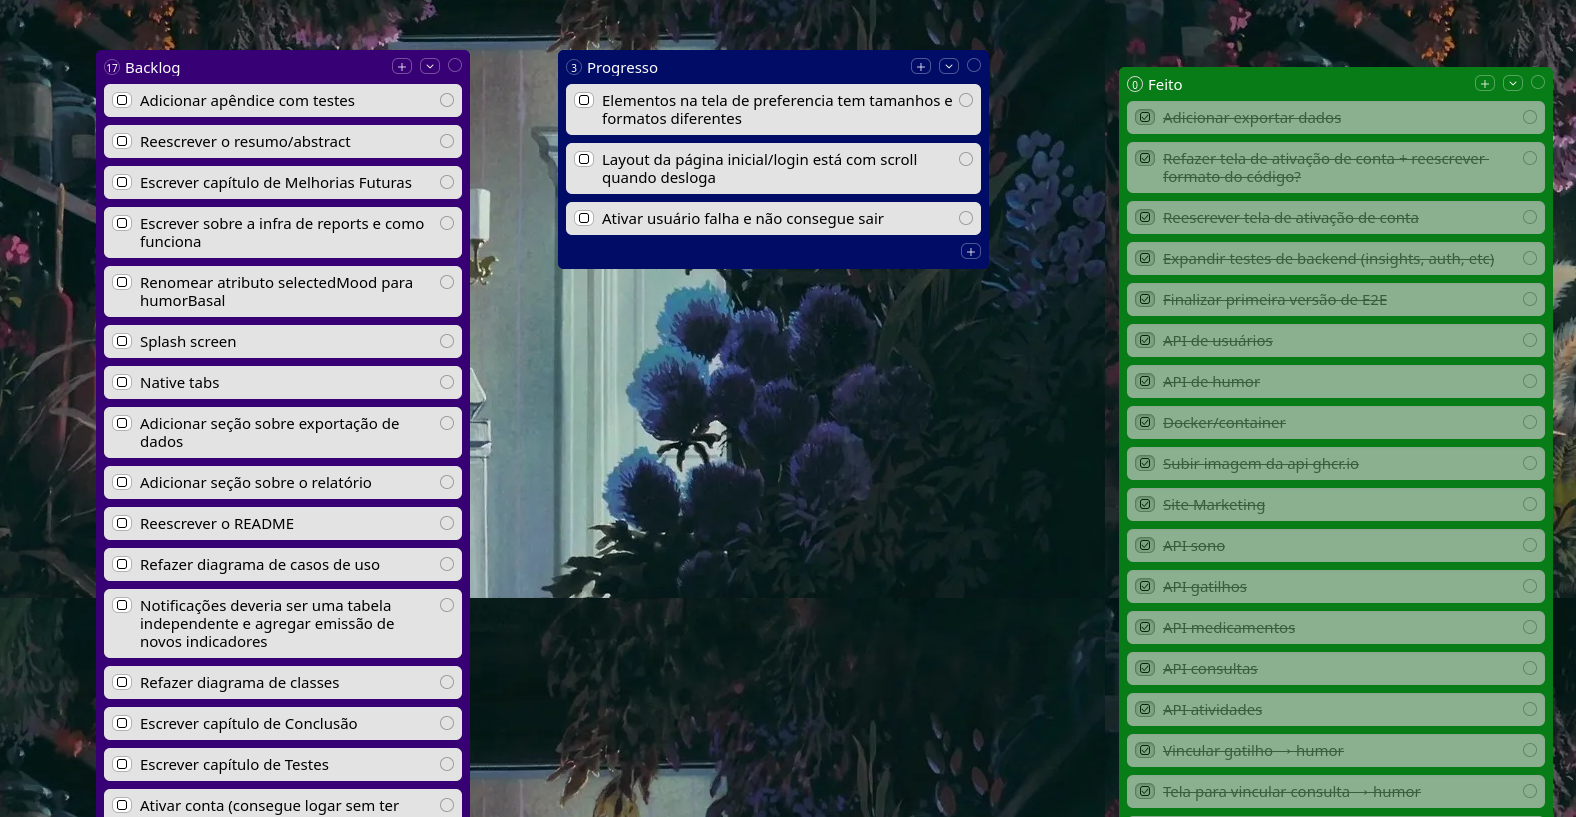
\includegraphics[width=0.90\textwidth,keepaspectratio]{kanban.png}
\source{Elaborado pelo autor (2026)}
\end{figure}

Por serem princípios, e não procedimentos, os valores ágeis não são aplicados
diretamente: precisam ser instanciados em métodos concretos, como o
\textit{Kanban} e o \textit{Scrum}. O \textit{Scrum} organiza o trabalho em
papéis e cerimônias (\textit{Product Owner}, \textit{Scrum Master},
\textit{dailies}, \textit{sprint reviews}) pensados para coordenar uma equipe.
O \textit{Kanban}, por sua vez, baseia-se na visualização do fluxo de trabalho,
como demonstrado na Figura \ref{fig:kanban} e na limitação de tarefas em progresso,
sem pressupor uma estrutura de equipe \cite{Anderson:2010}.

Por ser um método não prescritivo, o \textit{Kanban} não define um ciclo de
vida de desenvolvimento; ele organiza a execução do trabalho definido por outro
modelo. Isso permite que as tarefas sejam priorizadas, ajustadas ou
redefinidas, conforme a evolução do projeto, característica especialmente útil
quando há apenas um desenvolvedor responsável por todas as etapas do processo.

Com base nesse panorama, o presente trabalho adotou um misto: utiliza o modelo
incremental estrutura o ciclo de desenvolvimento em entregas funcionais
sucessivas; os princípios ágeis orientam as decisões, priorizando em entregas
funcionais sucessivas; os princípios ágeis orientam as decisões, priorizando a
entrega contínua de valor e a adaptação a mudanças; e o \textit{Kanban}
organiza a execução por meio de um quadro que separa o que precisa ser feito, o
que está em andamento e o que já foi concluído, limitando a quantidade de
tarefas em progresso. Essa combinação mantém o controle sobre o andamento e a
qualidade do produto sem os entraves de cerimônias e papéis pensados para
equipes, o que a torna adequada a um desenvolvimento individual.

\section{Metodologia de Pesquisa}

Entende-se por pesquisa científica, a investigação de um fenômeno, de forma a
encontrar a solução para algum problema \cite{Coelho:2020}. Portanto, a
metodologia científica se torna o conjunto de procedimentos para esta
investigação, cujo qual perpassa a coleta e análise de dados. Neste capítulo,
abordaremos as metodologias adotadas e suas respectivas justificativas, para
além dos dados encontrados para tal.

\subsection{Tipo de Pesquisa}

Segundo \cite{Lakatos:2022}, a pesquisa científica pode ser classificada
quanto aos seus objetivos como exploratória, descritiva ou explicativa. Este
trabalho caracteriza-se principalmente como uma pesquisa aplicada de natureza
exploratória, uma vez que busca investigar práticas, limitações e necessidades
relacionadas a ferramentas digitais para acompanhamento emocional, com o
objetivo de desenvolver uma solução tecnológica prática.

Conforme \cite{Gerhardt:09}, a pesquisa aplicada visa gerar conhecimento para
aplicação direta em problemas específicos, com interesse prático e utilitário,
sendo comum em projetos de desenvolvimento de \textit{software}, especialmente
nas áreas de Sistemas de Informação e Ciência da Computação, nas quais o
produto final visa resolver uma demanda concreta do público-alvo. Nesse
contexto, a coleta de dados junto a potenciais usuários orienta as decisões do
projeto, conforme detalhado a seguir.

\subsection{Instrumento de coleta de dados}

Como instrumento de coleta de dados, optou-se pela aplicação de um questionário
estruturado, elaborado com o intuito de compreender hábitos, preferências e
resistências de usuários em relação ao uso de aplicativos voltados para o
acompanhamento emocional e práticas de autorreflexão.

A escolha do questionário se justifica pela sua abrangência, agilidade na
coleta de dados e facilidade de análise quantitativa e qualitativa. Além disso,
como a amostra é composta por usuários potenciais, a aplicação do questionário
de forma digital por meio de um formulário online permite alcançar um público
mais amplo com baixo custo e maior comodidade \cite{EvansAndMathur:2005}.

O questionário, disponível no Apêndice B, foi divulgado de forma aberta entre 7
e 16 de julho de 2025 e obteve 48 respostas. Trata-se, portanto, de uma amostra
por conveniência, cujos resultados descrevem o grupo respondente e não podem
ser generalizados. A amostra é composta majoritariamente por mulheres (32
respostas; 66,7\%), com idades entre 18 e 30 anos (21; 43,8\%), 31 e 45 anos
(14; 29,2\%), 46 e 60 anos (11; 22,9\%) e acima de 60 anos (2; 4,2\%). Dos
participantes, 18 (37,5\%) relataram diagnóstico relacionado à saúde mental.
Como a divulgação foi aberta e o tame envolve saúde mental e experiências
subjetivas, a primeira pergunta ``Você já teve algum interesse ou experiência
com o monitoramento do seu humor ou estado emocional?'', buscava situar os
respondentes quanto ao perfil de potencias usuários.

Nessa pergunta, apenas 4 participantes (8,3\%) afirmaram não ter interesse nem
experiência, enquanto 25 (52,1\%) afirmaram ter interesse, mas nunca ter
tentado. Na pergunta específica sobre histórico, 26 dos 47 respondentes
(55,3\%) já monitoraram o humor em algum momento da vida, de forma regular,
ocasional ou interrompida. A Tabela~\ref{tab:survey-summary} sintetiza os
resultados mais relevantes para as decisões do projeto.

\begin{table}[H]
    \centering
    \caption{Síntese dos resultados do questionário}
    \label{tab:survey-summary}
    \small
    \renewcommand{\arraystretch}{1.3}   % respiro vertical
    \setlength{\aboverulesep}{0.4ex}
    \setlength{\belowrulesep}{0.4ex}
    \begin{tabularx}{\textwidth}{@{}>{\raggedright\arraybackslash\hsize=1.25\hsize}X
                                   >{\raggedright\arraybackslash\hsize=0.75\hsize}X
                                   r r@{}}
        \toprule
        \textbf{Pergunta} & \textbf{Resposta} & \textbf{Freq./base} & \textbf{\%} \\
        \midrule
        Interesse ou experiência com monitoramento de humor
            & ``Tenho interesse, mas nunca tentei'' & 25/48 & 52,1 \\
        \cmidrule[0.25pt]{1-4}
        Já monitorou o humor em algum momento da vida
            & Sim (regular, ocasional ou interrompido) & 26/47 & 55,3 \\
        \cmidrule[0.25pt]{1-4}
        Já recebeu diagnóstico relacionado à saúde mental
            & Sim & 18/48 & 37,5 \\
        \midrule
        Motivo mais citado para abandono ou dificuldade\textsuperscript{1}
            & Esquecimento & 14/25 & 56,0 \\
        \cmidrule[0.25pt]{1-4}
        Segundo motivo mais citado\textsuperscript{1}
            & Falta de tempo & 10/25 & 40,0 \\
        \cmidrule[0.25pt]{1-4}
        Terceiro motivo mais citado\textsuperscript{1}
            & Preocupações com privacidade & 6/25 & 24,0 \\
        \midrule
        Importância de ter controle total sobre os próprios dados
            & Nota máxima (5) & 32/47 & 68,1 \\
        \cmidrule[0.25pt]{1-4}
        Preferência de armazenamento
            & Apenas no dispositivo (sem nuvem) & 14/48 & 29,2 \\
        \cmidrule[0.25pt]{1-4}
        Conforto em compartilhar dados anonimamente para pesquisa
            & Sim & 28/48 & 58,3 \\
        \midrule
        Tom de comunicação preferido
            & ``Acolhedor e empático'' & 18/48 & 37,5 \\
        \cmidrule[0.25pt]{1-4}
        Utilidade de o aplicativo avisar sobre possíveis ciclos de humor
            & Sim & 36/48 & 75,0 \\
        \bottomrule
    \end{tabularx}
    \par\vspace{2pt}
    {\footnotesize \textsuperscript{1} Resposta de múltipla escolha; base: 25
    respondentes que relataram motivos (excluídas respostas como ``nunca fiz'').}
    \source{Elaborado pelo autor (2026), dados de 2025}
\end{table}

% TODO: cite this paragraph on limitations/conclusions/future works

Quanto à detecção de padrões, 33 participantes (68,8\%) acreditam que um
aplicativo pode ajudar a perceber padrões emocionais que normalmente não
notariam, e outros 13 (27,1\%) responderam ``talvez''. Dois participantes
mencionaram espontaneamente a visualização gráfica da evolução do humor, como
em ``seria legal ver um gráfico semanal ou mensal do meu humor''. Quanto aos
ciclos de humor, 36 participantes (75,0\%) consideraram útil que o aplicativo
os identifique e avise, e 10 (20,8\%) condicionaram a utilidade à precisão.
Contudo, quando avaliada como funcionalidade em escala de 1 a 5, a detecção de
ciclos obteve média 2,93, com 31,8\% de notas 4 ou 5 (considerando total de 44
respondentes). O resultado indica interesse no conceito, mas com cautela quanto
à sua execução, o que reforça a necessidade de comunicar com clareza a
incerteza das inferências.

Em relação à privacidade, 32 dos 47 respondentes (68,1\%) atribuíram a nota
máxima à importância de ter controle total sobre os próprios dados, e a
privacidade foi o terceiro motivo mais citado para abandono (24,0\%). Essa
percepção está alinhada com a literatura sobre saúde digital:
\citet{Iwaya:22} argumentam que a ausência de mecanismos transparentes de
consentimento, controle e anonimização pode minar a confiança dos usuários em
aplicativos de bem-estar, especialmente em contextos sensíveis como saúde
mental.

Ao mesmo tempo, não houve consenso sobre o armazenamento: 29,2\% preferem
guardar os dados apenas no dispositivo, 22,9\% aceitam a nuvem criptografada,
22,9\% são indiferentes desde que possam acessar e exportar, e 25,0\% não tem
preferência. Já 58,3\% se sentiriam confortáveis em compartilhar dados de forma
anônima para pesquisa, e 29,2\% responderam que dependeria do tipo de dado.

Por fim, quanto ao tom, o ``acolhedor e empático'' foi o mais frequente
(37,5\%), seguido do ``neutro e objetivo'' (25,0\%), do ``clínico e
profissional'' (20,8\%) e do ``lúdico e leve'' (12,5\%). Embora o tom acolhedor
se destaque, a ausência de preferência majoritária indica que a linguagem do
aplicativo deve ser cuidadosa, sem pressupor um único registro. Em relação à
frequência, 20 participantes (41,7\%) afirmaram conseguir registrar o humor uma
vez ao dia e 12 (25,0\%), duas vezes, o que sustenta um registro leve e
recorrente.

\subsection{Análise de Similares}

% TODO: reescrever, arrumar citação
A metodologia trata-se de uma avaliação sobre os sistemas relacionados ao tema
proposto, observando e levantando desafios e possibilidades, validação de
\textit{softwares} e a satisfação dos usuários (Martins, 2018). Seguindo assim,
foram pesquisados sistemas similares encontrados na internet com o objetivo de
realizar uma revisão crítica-reflexiva, analisando os aplicativos que oferecem
algum tipo de diário digital de humor, ou permite algum acompanhamento
reflexivo de variações de emoções.

Para realizar esse processo, de forma a simular também um usuário, foi
pesquisado na Google Play Store \footnote{Google Play Store --- Disponível em:
https://play.google.com}, por \textit{mood tracker}, retornando centenas de
resultados. Nesse quesito, estabeleceu os seguintes critérios objetivos: (1)
pode ser um aplicativo em português ou inglês; (2) o aplicativo tem que
apresentar algum tipo de gráfico das entradas feitas (3) tem que possuir
entrada textual.

\subsubsection{Baseline}

O Baseline é um aplicativo de código aberto voltado ao acompanhamento do
bem-estar emocional por meio de uma abordagem minimalista. A ferramenta permite
o registro diário de humor utilizando entradas textuais ou gravações de áudio,
além de disponibilizar notificações personalizadas e revisões periódicas dos
registros realizados.

\begin{figure}[H]
\centering
\caption{Aplicativo Baseline}
\label{fig:screenshot-baseline}
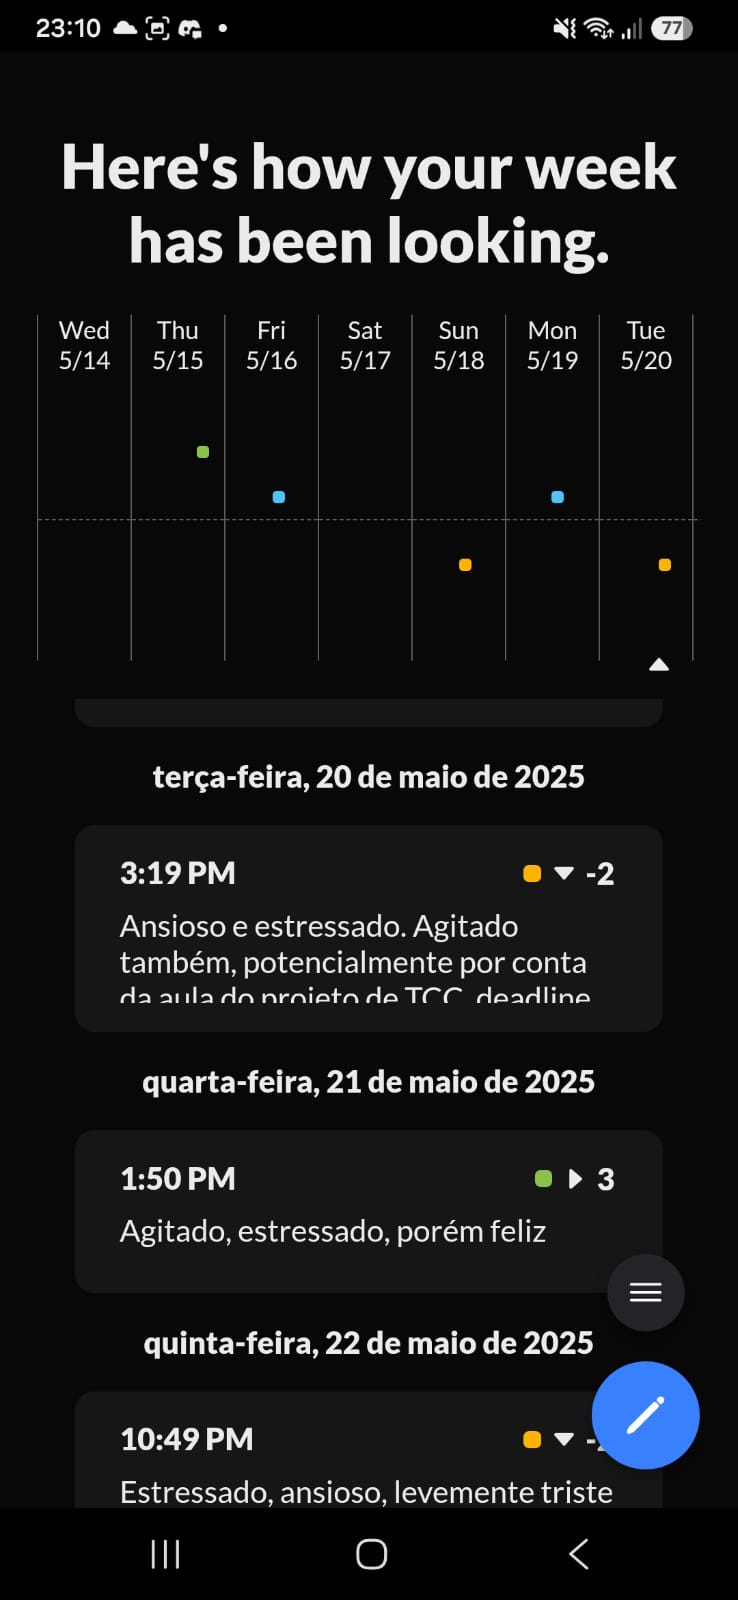
\includegraphics[width=0.40\textwidth,height=0.40\textheight,keepaspectratio]{screenshot-baseline.jpeg}
\source{Elaborado pelo autor (2026)}
\end{figure}

Entre os aspectos observados, destaca-se a natureza open-source da aplicação,
característica que favorece a transparência e a possibilidade de adaptação por
terceiros. Sua interface apresenta baixo nível de complexidade e reduz a
quantidade de interações necessárias para o registro das informações.
Entretanto, nota-se que o sistema não oferece visualizações temporais avançadas
nem mecanismos de personalização mais aprofundados. Além disso, o
acompanhamento emocional é realizado principalmente por meio de uma pontuação
de humor, sem identificar ciclos emocionais ou relacionar registros a gatilhos
e intervenções específicas.

\subsubsection{DailyBeans}

O DailyBeans é um dos aplicativos de monitoramento de humor mais populares
disponíveis atualmente, possuindo como principal característica a simplicidade
de uso. Nota-se que  possui uma linguagem bem lúdica e informal, por exemplo, o
sistema utiliza o conceito de ``feijões'' representando o estado de humor do
usuário. Destaca-se que o aplicativo permite selecionar categorias de
sentimentos e adicionar atividades para preencher melhor o registro do estado
emocional do usuário para além de um ``Feliz'', ``Triste'', etc. Existe também uma
bastante vasta opções de categorias, cada qual com uma ilustração que
representa o que aquilo representa. O aplicativo também apresenta ``Temas
sazonais'', permitindo que o usuário customize cores, icones, e demais
informações. Um elemento interssante é que as informações adicionadas também
podem ser \textit{offlines}, até uma certa quantidade de entradas/registros,
necessitando de uma conta para poder continuar salvando os dados informados.

\begin{figure}[H]
\centering
\caption{Aplicativo DailyBeans}
\label{fig:screenshot-dailybeans}
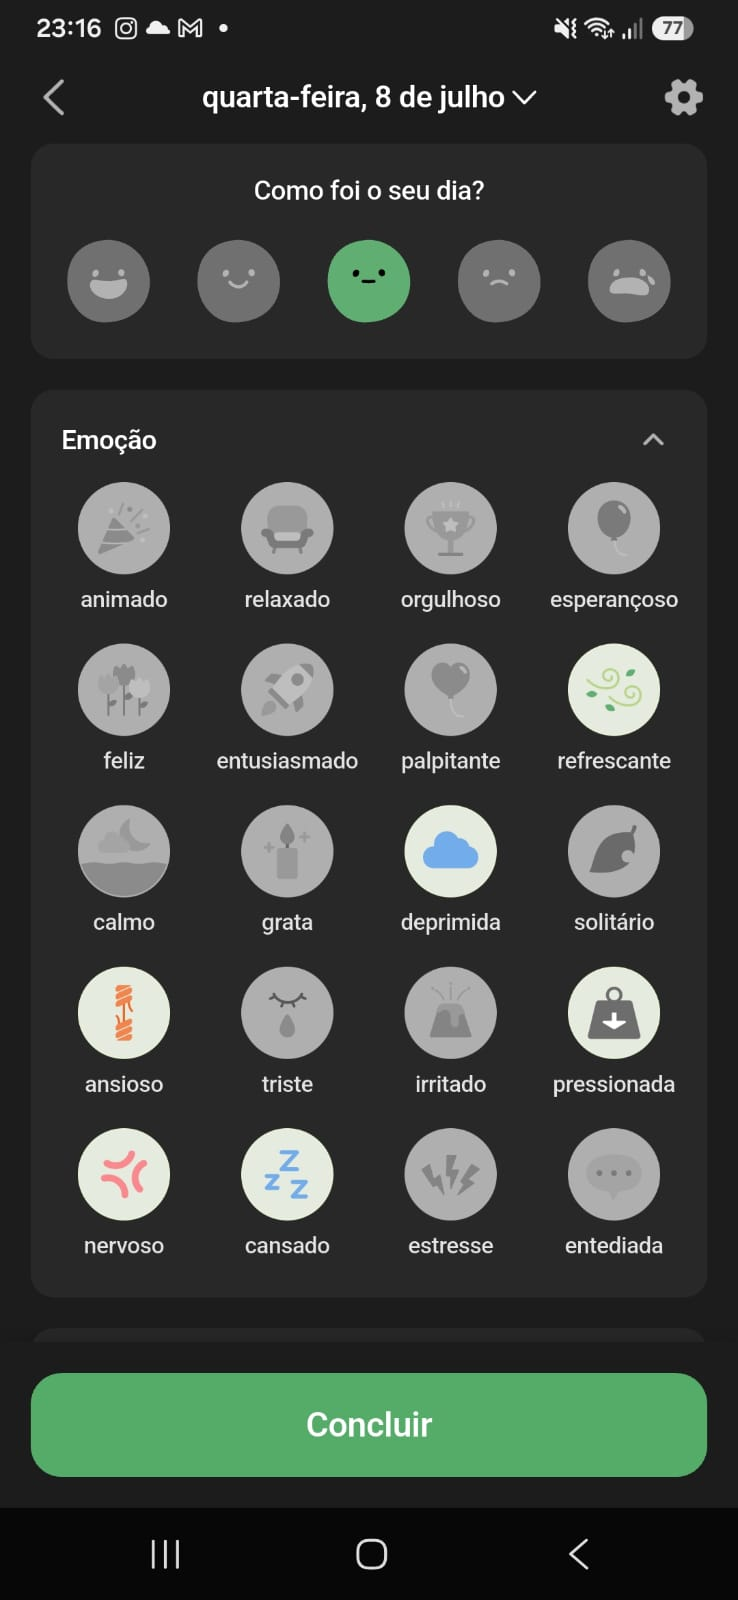
\includegraphics[width=0.40\textwidth,height=0.40\textheight,keepaspectratio]{screenshot-dailybeans.jpeg}
\source{Elaborado pelo autor (2026)}
\end{figure}

Entre suas funcionalidades, além do registro de humor e categorização de
atividades e sentimentos, o aplicativo conta com gráficos e históricos. Uma
interface bastante coesa e visualmente agradável. Um outro elemento é que o
aplicativo permite relacionar indicadores de sono com bastante precisão, como
poder indicar o momento que foi dormir, momento que acordou, anotações, etc. O
aplicativo permite adicionar pelo menos uma foto no plano gratuito, além de
indicar elementos como ``Qual o clima do dia'', se o usuário esteve com
``amigos'', ``familiares''.

Observa-se que o aplicativo possui código fechado e restringe parte de suas
funcionalidades mais avançadas à versão paga ou compras na Loja interna do
aplicativo para obter por exemplo, personalização de icones, adicionar mais
fotos. Além disso, o foco em registros rápidos reduz a flexibilidade para
inserção de reflexões textuais mais detalhadas, e uma exibição excessante de
anúncios atrapalha a utilização.

\subsubsection{DailyMood}

DailyMood é um aplicativo voltado ao registro cotidiano do estado emocional,
oferecendo uma solução enxuta para acompanhamento de humor. Sua proposta
baseia-se em uma interação mínima, permitindo que o usuário selecione
rapidamente o sentimento predominante do dia, sem a necessidade de descrições
extensas. Os registros são organizados em um calendário, o que facilita a
leitura histórica e a identificação de padrões emocionais ao longo do tempo.

\begin{figure}[H]
\centering
\caption{Aplicativo DailyMood}
\label{fig:screenshot-dailymood}
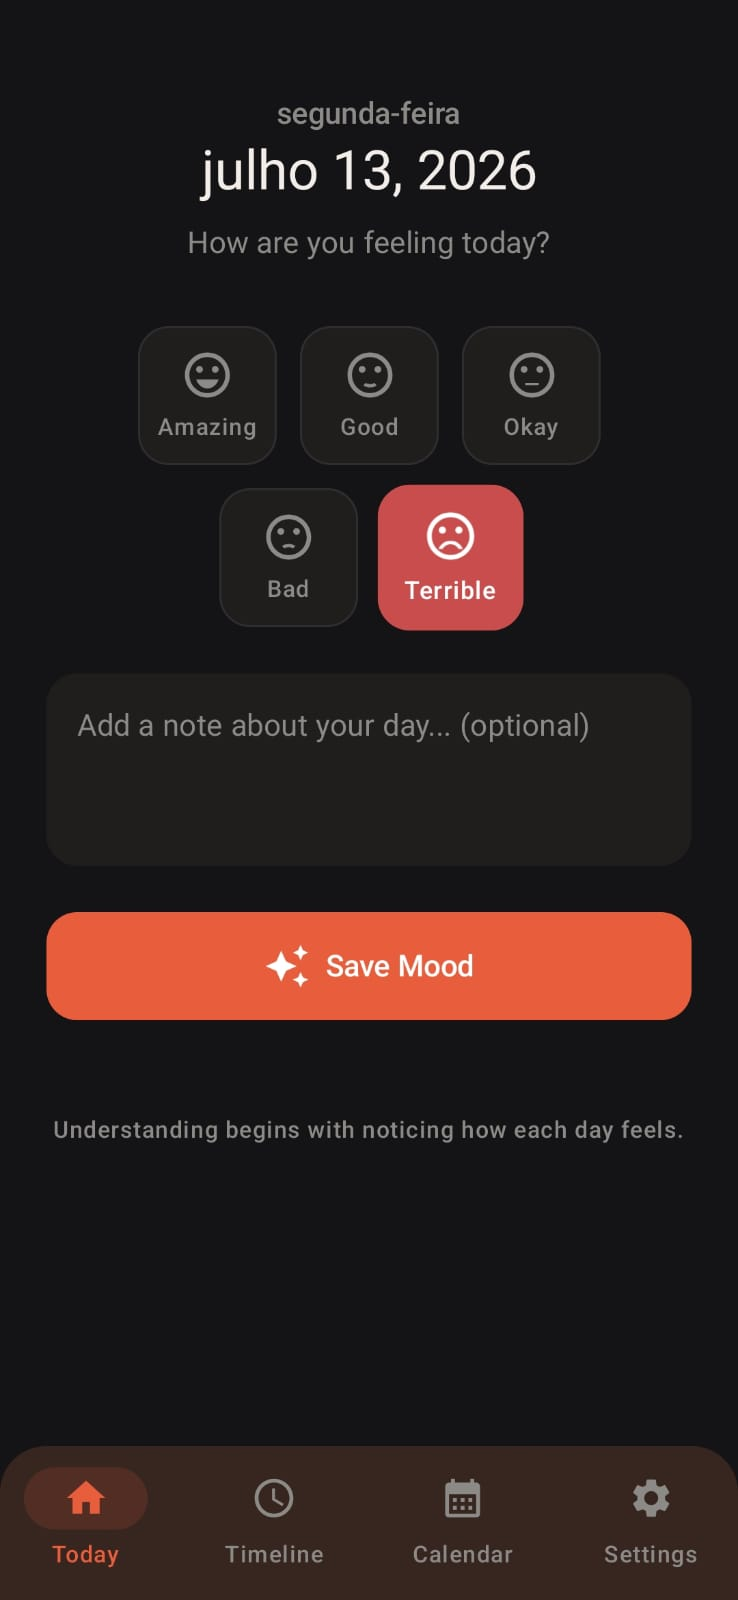
\includegraphics[width=0.40\textwidth,height=0.55\textheight,keepaspectratio]{screenshot-dailymood.jpeg}
\source{Elaborado pelo autor (2026)}
\end{figure}

Apesar dos recursos disponíveis, observa-se que é uma solução bastante simples.
Não existe outros recursos além de informar o humor predominante e uma
anotação. Um fator interessante é que não necessita de contas, rodando
completamente offline no dispositivo do usuário. Adicionalmente, apresenta
limitações relacionadas à exportação dos dados registrados e à personalização
das informações armazenadas.

\subsubsection{Reflectly}

O Reflectly é um aplicativo de diário pessoal que utiliza recursos de
inteligência artificial para promover práticas de autorreflexão e
acompanhamento emocional. Sua proposta enfatiza a experiência do usuário e a
construção de narrativas pessoais a partir dos registros realizados.

Entre suas funcionalidades estão entradas textuais livres, perguntas guiadas
diárias, análises emocionais automatizadas e personalização visual da
interface. O sistema apresenta uma experiência moderna e intuitiva,
incentivando o uso contínuo por meio de elementos de engajamento.
Um ponto interessante é o fato do aplicativo separar o ``humor'' dos
``sentimentos'', permitindo que os usuários avaliem ambos de forma
independente.

\begin{figure}[H]
\centering
\caption{Aplicativo Reflectly}
\label{fig:screenshot-reflectly}
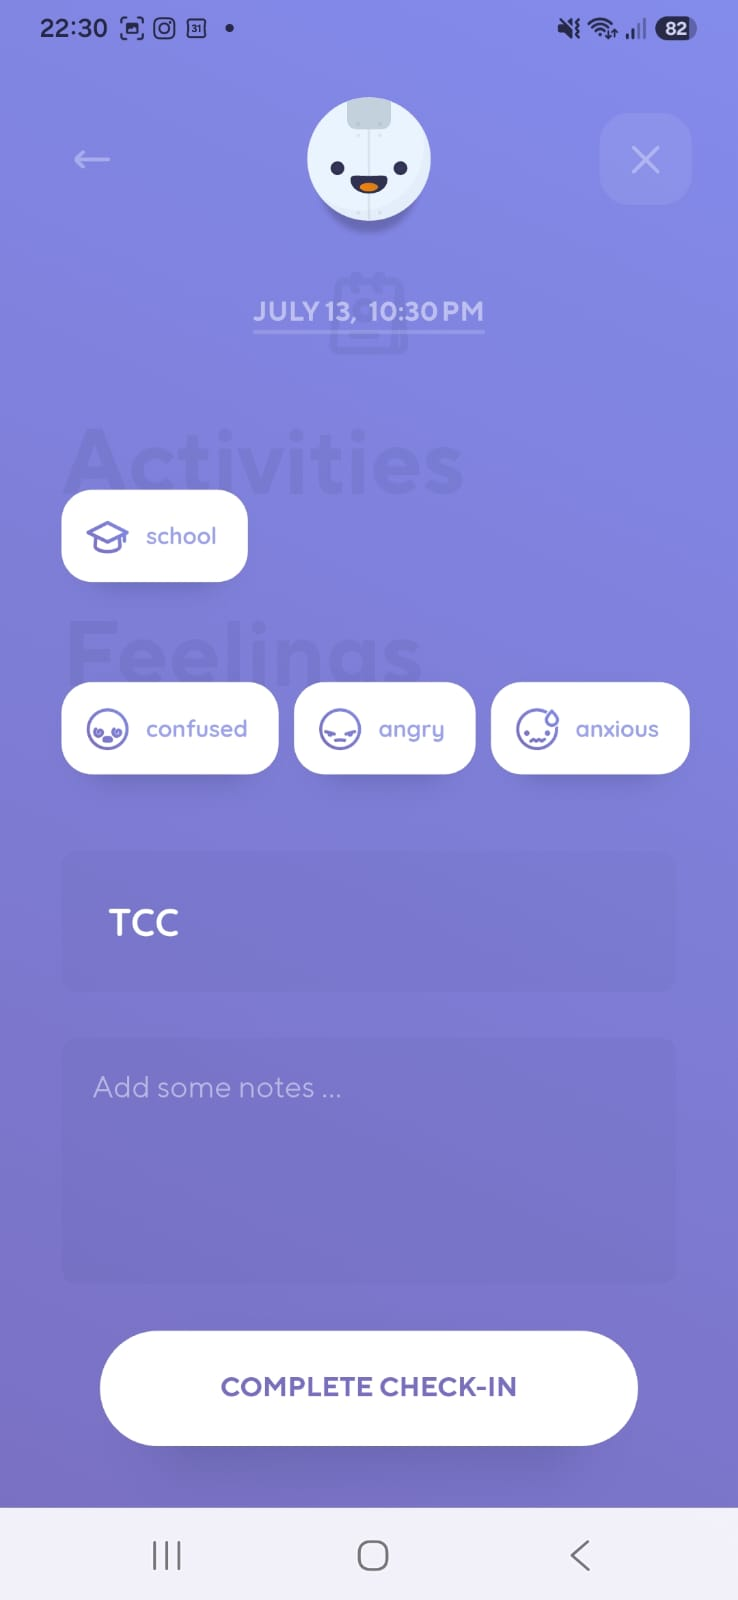
\includegraphics[width=0.40\textwidth,height=0.55\textheight,keepaspectratio]{screenshot-reflectly.jpeg}
\source{Elaborado pelo autor (2026)}
\end{figure}

Como pontos observados, destaca-se o fato de ser uma solução proprietária e
dependente de coleta significativa de dados para alimentar seus mecanismos de
análise. Outro ponto observado é o fato de que o aplicativo apresenta
elementos como estatísticas e histórico, porém necessita de uma conta
paga para acessar esses recursos.

Além disso, sua abordagem está mais voltada ao diário pessoal do que
ao acompanhamento sistemático de indicadores de saúde mental.

\subsubsection{eMoods}

O \textit{eMoods} é um aplicativo de registro de humor especificamente para
pessoas com TAB. O aplicativo tem uma interface bem compacta, bastante
poluída visualmente, em estilo formulário de entrada de dados.

O aplicativo consegue registrar dados de sono, além de perguntas como
ansiedade, estado depressivo, e outras coisas como ``você praticou higiene
pessoal?'', ``você tomou medicamentos?'', ``você se alimentou bem?'' e afins.
Um ponto destacado é que o aplicativo também permite exportar os dados em
formato CSV e gerar relatórios em formato PDF.

\begin{figure}[H]
\centering
\caption{Aplicativo eMoods}
\label{fig:screenshot-emoods}
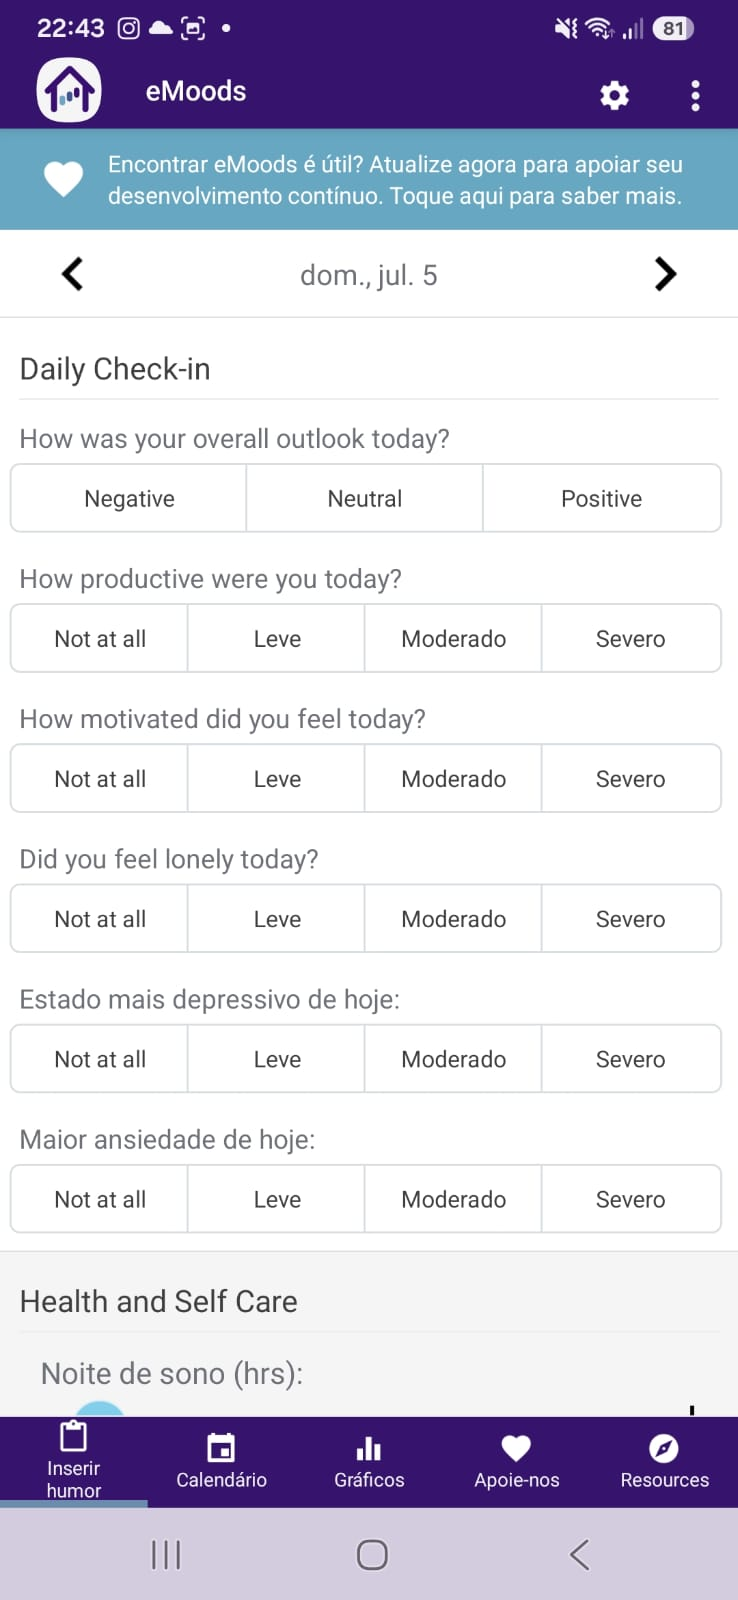
\includegraphics[width=0.40\textwidth,height=0.55\textheight,keepaspectratio]{screenshot-emoods.jpeg}
\source{Elaborado pelo autor (2026)}
\end{figure}

Entretanto, a aplicação apresenta uma experiência do usuário um tanto confusa,
possuindo interface bastante poluída quando comparada a soluções mais
novas/contemporâneas. Também não oferece suporte para registros textuais
extensos ou entradas por voz, além de simular um formulário.

\FloatBarrier

\subsection{Análise comparativa}

Coletando essa lista de aplicações, é possível então dispor as funcionalidades
mais relevantes de cada aplicação da seguinte forma:

\begin{table}[H]
    \centering
    \caption{Comparativo de funcionalidades entre aplicativos analisados}
    \label{tab:comparativo_apps}
    \begin{tabular}{|l|c|c|c|c|c|}
        \hline
        Funcionalidade &
        Baseline &
        DailyBeans &
        DailyMood &
        Reflectly &
        eMoods \\

        \hline
        Registro de humor & Sim & Sim & Sim & Sim & Sim \\
        \hline
        Registro de sono & Não & Não & Não & Não & Sim \\
        \hline
        Texto livre & Sim & Parcial & Sim & Sim & Sim \\
        \hline
        Gráficos & Não & Sim & Sim & Sim & Sim \\
        \hline
        Gatilhos/intervenções & Não & Parcial & Não & Não & Parcial \\
        \hline
        Exportação de dados & Sim & Parcial & Parcial & Parcial & Sim \\
        \hline
        Código aberto & Sim & Não & Não & Não & Não \\
        \hline
    \end{tabular}
    \source{Elaborado pelo autor (2026)}
\end{table}

Com esses dados em mente, podemos compreender alguns elementos fundamentais:
poucos sistemas analisados são \textit{open-source}, o que indica que, em sua
grande maioria, são sistemas comerciais. A maior parte dos sistemas também
oferecem algum aspecto de pagamento, bloqueando funcionalidades importantes
atrás de algum tipo de modelo de subscrição. Existe também o fato de
personalização e de exportação de dados, que poucos ou nenhum sistema oferece,
o que faz com que o sistema não tenha portabilidade dos dados inseridos,
criando assim, um \textit{walled garden}, ou um jardim fechado --- uma técnica de
fazer com que o usuário não consiga migrar entre sistemas, prendendo-o a usar
aquela aplicação já que seus dados estão lá.

\subsection{Relação entre os dados do questionário e análise de similares}

A análise dos sistemas similares, quando considerada em conjunto com os dados
coletados por meio do questionário, revela lacunas e oportunidades relevantes
para o desenvolvimento de uma nova solução. Observa-se, por exemplo, que a
maior parte das ferramentas disponíveis no mercado segue modelos comerciais,
frequentemente com funcionalidades essenciais bloqueadas por sistemas de
pagamento ou assinaturas. Além disso, é comum que tais sistemas sejam fechados,
sem disponibilização de código-fonte ou possibilidade de exportação dos dados
inseridos, o que configura uma prática de \textit{walled garden}, dificultando
a migração entre plataformas e restringindo a autonomia dos usuários sobre suas
próprias informações.

Esses aspectos, quando contrastados com o interesse expressivo dos respondentes
por visualizar padrões emocionais ao longo do tempo e por maior personalização,
sugerem direções claras para o desenvolvimento de um sistema que não apenas
atenda a essas demandas, mas também adote princípios de transparência, abertura
e controle por parte do usuário. A seguir, serão discutidas as decisões de
projeto que nortearam a construção da ferramenta proposta, baseadas tanto nas
limitações identificadas nos sistemas existentes quanto nas necessidades e
expectativas manifestadas pelo público-alvo da pesquisa.

\chapter{Nexo}

O aplicativo proposto por esse trabalho, denominado ``Nexo'', se propõe a ser uma
aplicação para dispositivos móveis, de forma a preencher essas lacunas
demonstradas tanto pelo questionário, quanto também tentando preencher as
questões analisadas em outros sistemas similares. Como mencionado
anteriormente, o sistema é direcionado para pessoas com TAB, embora, ele também
possa atuar isoladamente como um aplicativo de registro de humor, e portanto, o
nome reflete essa escolha. A lógica é, de um aplicativo que consegue conectar
diversos pontos, que em um primeiro momento parecem soltos: sono, rotina,
práticas, humor, gatilhos.

A partir das demandas identificadas na pesquisa e dos princípios estabelecidos
para este projeto, delineia-se um sistema de monitoramento de humor centrado no
usuário, com ênfase em personalização, privacidade e utilidade reflexiva. O
funcionamento do sistema parte da premissa de que o humor não é uma variável
universal, mas sim composto por elementos subjetivos que variam entre
indivíduos. Assim, fundamentalmente para cada entrada no diário, o usuário pode
indicar que componentes de humor ele percebe em vigência naquele momento, como
``raiva'', ``tristeza'', ``felicidade'', etc., elementos que ele considera mais
representativos de seu estado emocional, permitindo um mapeamento mais fiel da
sua experiência.

O monitoramento, pode ser gerado em diversos momentos do dia, o que torna o
aplicativo mais flexível, ao invés de uma única entrada no dia. O usuário pode
também anotar para cada momento, algo relevante, através de escrita livre, e
usar uma escala que possa indicar o que ele percebe como indicadores dos níveis
de energia, estresse e ansiedade. Associado a isso, o sistema permitirá a
entrada de gatilhos e eventos significativos, sejam positivos ou negativos, que
poderão ser posteriormente correlacionados com os estados de humor, permitindo
identificar padrões ou ciclos. Esses dados podem ser correlacionados/vinculados
com ``práticas'' ou ``intervenções'', como fármacos, psicoterapia, atividades
físicas.

Outro ponto essencial é a exportação de dados em formatos acessíveis, como o
formato CSV \cite{Shafranovich_2005} \footnote{Formato de arquivo onde cada
coluna é separado por um delimitador, por exemplo: vírgulas, ponto-e-vírgula,
apresentado no RFC 4180}, garantindo que o usuário tenha controle e mobilidade
sobre suas informações, algo frequentemente negligenciado em sistemas fechados.
Além disso, a ferramenta é por inteiro \textit{software} livre, garantindo
transparência de funcionamento, possibilidade de auditoria e fomento a
melhorias comunitárias, especialmente importantes no contexto de tecnologias
sensíveis à saúde mental. Essas características formam a base de um sistema
comprometido com o bem-estar, o respeito à individualidade e a soberania dos
dados pessoais.

Com base nas funcionalidades listadas, pode-se definir os requisitos funcionais
e não funcionais no qual o sistema deve necessitar.

\section{Classificação dos Requisitos}

Como observado por \cite[p.~58]{sommerville:2010}, ``Os requisitos de um sistema são
as descrições dos serviços que o sistema deve prestar e as restrições à sua
operação''. Portanto, requisitos são declarações articuladas descrevendo de
forma clara o que o sistema deve ser capaz de fazer para satisfazer as
necessidades postas anteriormente. São definidas em duas categorias: requisitos
funcionais que descrevem o comportamento e funções do sistema e requisitos não
funcionais que descrevem os critérios específicos que podem ser usados para
avaliar o bom funcionamento do sistema. A separação entre requisitos funcionais
e não funcionais permite uma estrutura clara para priorização, testes e
validação do projeto, respeitando tanto os objetivos técnicos quanto éticos da
proposta. Logo a seguir, serão abordados com mais detalhes cada um deles.

\subsection{Requisitos funcionais}

Os requisitos funcionais dizem respeito às funcionalidades centrais do sistema,
ou seja, declarações de tudo o que o sistema deve e está proposto a fazer e
reagir. Sommerville reforça esse aspecto:

\begin{quote}

  Os requisitos funcionais de um sistema descrevem o que ele deve fazer. Eles
  dependem do tipo de software a ser desenvolvido, de quem são seus possíveis
  usuários e da abordagem geral adotada pela organização ao escrever os
  requisitos. Quando expressos como requisitos de usuário, os requisitos
  funcionais são normalmente descritos de forma abstrata, para serem
  compreendidos pelos usuários do sistema.

  \cite[p.~59]{sommerville:2010}
\end{quote}

Portanto, diante das funcionalidades previstas, que foram brevemente listadas,
no Quadro~\ref{tab:requisitos_funcionais} é apresentado os requisitos que o
sistema deve fornecer:

\newpage

% TODO: Add this to the list of tables
\begin{longtable}{| p{.20\textwidth} | p{.30\textwidth} | p{.40\textwidth} |}
    \caption{Requisitos funcionais}
    \label{tab:requisitos_funcionais} \\
        \hline
        N° & Requisito & Descrição \\
        \hline
        \endfirsthead
        \hline
        N° & Requisito & Descrição \\
        \hline
        \endhead
        \endfoot

        [RF01] &
        Login &
        O sistema deve ser capaz de realizar login com email e senha \\

        \hline

        [RF02] &
        Redefinir senha &

        O sistema permite que o usuário redefina a sua senha, mediante informar
        o email usado \\

        \hline

        [RF03] &
        Cadastro &
        O sistema deve permitir que o usuário crie uma conta \\

        \hline

        [RF04] &
        Desconectar &
        O sistema permite que o usuário faça logout do sistema \\

        \hline

        [RF05] &
        Manter humor &
        O usuário deve poder registrar e atualizar seu estado emocional
        conforme a necessidade \\

        \hline

        [RF06] &
        Registrar gatilho &
        O sistema deve permitir associar sentimentos ou eventos específicos que
        influenciam o humor \\

        \hline

        [RF07] &
        Visualizar histórico &
        O usuário deve ter acesso aos registros anteriores de humor e demais
        tipos de dados como Gatilho, Sono, etc. \\

        \hline

        [RF08] &
        Visualizar detalhes do dia &
        O sistema deve permitir expandir e consultar dados específicos de um
        determinado dia \\

        \hline

        [RF09] &
        Visualizar registros de humor recente &
        O usuário deve poder visualizar os ultimos registros de humor como
        forma de ler \\

        \hline

        [RF10] &
        Manter registro de sono &
        O sistema deve permitir que o usuário possa cadastrar registros de sono \\

        \hline

        [RF11] &
        Manter ações de cuidado &
        O usuário deve poder cadastrar ações de cuidado (atividade, medicamentos, consultas) \\

        \hline

        [RF12] &
        Exportar dados &
        O sistema deve oferecer uma funcionalidade para exportar os dados
        registrados \\

        \hline

        [RF13] &
        Registrar que um medicamento foi tomado &
        O usuário pode marcar que um determinado medicamento foi tomado
        mediante que foi cadastrado \\

        \hline

        [RF14] &
        Associar humor à um gatilho &
        O sistema deve permitir que o usuário vincule um humor específico com
        um gatilho \\

        \hline

        [RF15] &
        Associar consulta com um humor ou gatilho &
        O sistema deve permitir vincular uma consulta específica a um
        gatilho ou humor registrado \\

        \hline

        [RF16] &
        Gerar um relatório com os últimos dados &
        O usuário deve selecionar um período e gerar/exportar um relatório com
        os últimos dados  \\

        \hline
        \multicolumn{3}{c}{\small Fonte: Elaborado pelo autor (2026)} \\
\end{longtable}

\subsection{Requirementos não funcionais}

De acordo com \cite[p.~89]{sommerville:2010}: ``Requisitos não funcionais são
restrições sobre os serviços ou funções oferecidas pelo sistema''. Ou seja,
definem os critérios de qualidade que o sistema deve seguir, abrangendo
aspectos como segurança, usabilidade, desempenho e manutenção. Neste projeto,
destacam-se especialmente a preservação da privacidade do usuário, a
transparência proporcionada pelo código aberto e a possibilidade de utilização
offline, o que garante acessibilidade mesmo em contextos de conectividade
limitada.

\begin{longtable}{| p{.20\textwidth} | p{.30\textwidth} | p{.40\textwidth} |}
    \caption{Requisitos não funcionais}
    \label{tab:requisitos_nao_funcionais} \\
        \hline
        N° & Requisito & Descrição \\
        \hline
        \endfirsthead
        \hline
        N° & Requisito & Descrição \\
        \hline
        \endhead
        \endfoot

        [RNF01] &
        Usabilidade &

        O sistema deve possuir uma interface intuitiva e acessível para
        usuários leigos em tecnologia, com navegação fluída e confirmações
        visuais após cada interação importante \\

        \hline

        [RNF02] &
        Desempenho &

        O tempo de resposta entre a entrada do usuário e a resposta do sistema
        deve ser inferior a 1 segundo; O carregamento do histórico semanal e
        visualizações de ciclos anteriores deve ocorrer em no máximo 2
        segundos. \\

        \hline

        [RNF03] &
        Segurança &

        Os dados do usuário devem ser armazenados de forma criptografada; O
        sistema deve exigir autenticação segura para acesso; A exportação de
        dados deve sempre exigir a confirmação do usuário \\
        \hline

        [RNF04] &
        Confiabilidade &

        O sistema deve garantir a persistência dos dados, mesmo em casos de
        falha de energia ou conexão; Os dados registrados devem ser armazenados
        automáticamente e sincronizados quando ouvir conexão \\

        \hline

        [RNF05] &
        Portabilidade &

        Todos os dados do usuário podem ser exportados a qualquer momento, em
        um formato de texto que permita que ele possa ler e interpretar,
        mediante compreensão mínima da linguagem/formato utilizado \\

        \hline

        [RNF06] &
        Privacidade &

        Nenhuma informação sensível do usuário deve ser compartilhada com
        terceiros e o sistema deve fornecer uma política de privacidade clara e
        acessível; Quaisquer alterações à mesma demanda que o usuário seja
        notificado \\

        \hline
        \multicolumn{3}{c}{\small Fonte: Elaborado pelo autor (2026)} \\
\end{longtable}

Com essas definições em mãos, pode-se avançar para a etapa de modelagem do
sistema, usando os requerimentos apresentados como fundação para o sistema.

\section{Modelagem}

De acordo com \cite{guedes:2022}, a modelagem de sistemas é uma etapa fundamental do
processo de desenvolvimento de software, pois permite representar graficamente
os principais elementos do sistema, seus comportamentos e interações. Essa
representação facilita a comunicação entre desenvolvedores, usuários e demais
envolvidos, servindo tanto como guia para implementação quanto como instrumento
de validação dos requisitos levantados. Através da modelagem, é possível
antever a estrutura do sistema, simular sua dinâmica e assegurar que ele
atenderá às necessidades específicas dos usuários.

Neste subcapítulo, são apresentados dois tipos principais de diagramas da
\textit{Unified Modeling Language} (UML) empregados na modelagem do sistema
proposto: o diagrama de casos de uso, que descreve as funcionalidades esperadas
a partir da perspectiva do usuário; o diagrama de classes, que estrutura os
elementos do domínio em termos de atributos e relacionamentos. Esses diagramas
complementam-se mutuamente, proporcionando uma visão abrangente do
comportamento e da arquitetura do sistema.

\subsection{Casos de Uso}

O diagrama de casos de uso é o mais geral, informal e simples de compreender
\cite{guedes:2022}. A base dele é o levantamento de requisitos e a pesquisa
realizada, e serve como o pontapé para todo o processo de modelagem.

O diagrama de casos de uso, apresenta de forma simples, os atores, que são
representações das entidades que interagem com o sistema (sejam eles usuários
finais ou outros sistemas), e os casos de uso, que são as funcionalidades que o
sistema oferece. Ambos são conectados por linhas de associação. O sistema
também é delimitado por um retângulo, que contém os casos de uso
\cite{ibm:2021}.

Ao final desse processo, essa modelagem é transformada em documentação, e no
Apêndice A deste documento, contém a mesma, oferecendo uma visão mais detalhada
para cada caso de uso, seus caminhos alternativos e caminhos de exceções.
Pode-se verificar que esse acaba por ser o diagrama mais basilar do projeto
inteiro \cite{guedes:2022}.

\begin{figure}[h]
\centering
\caption{Diagrama de Casos de Uso}
\label{fig:use-cases}
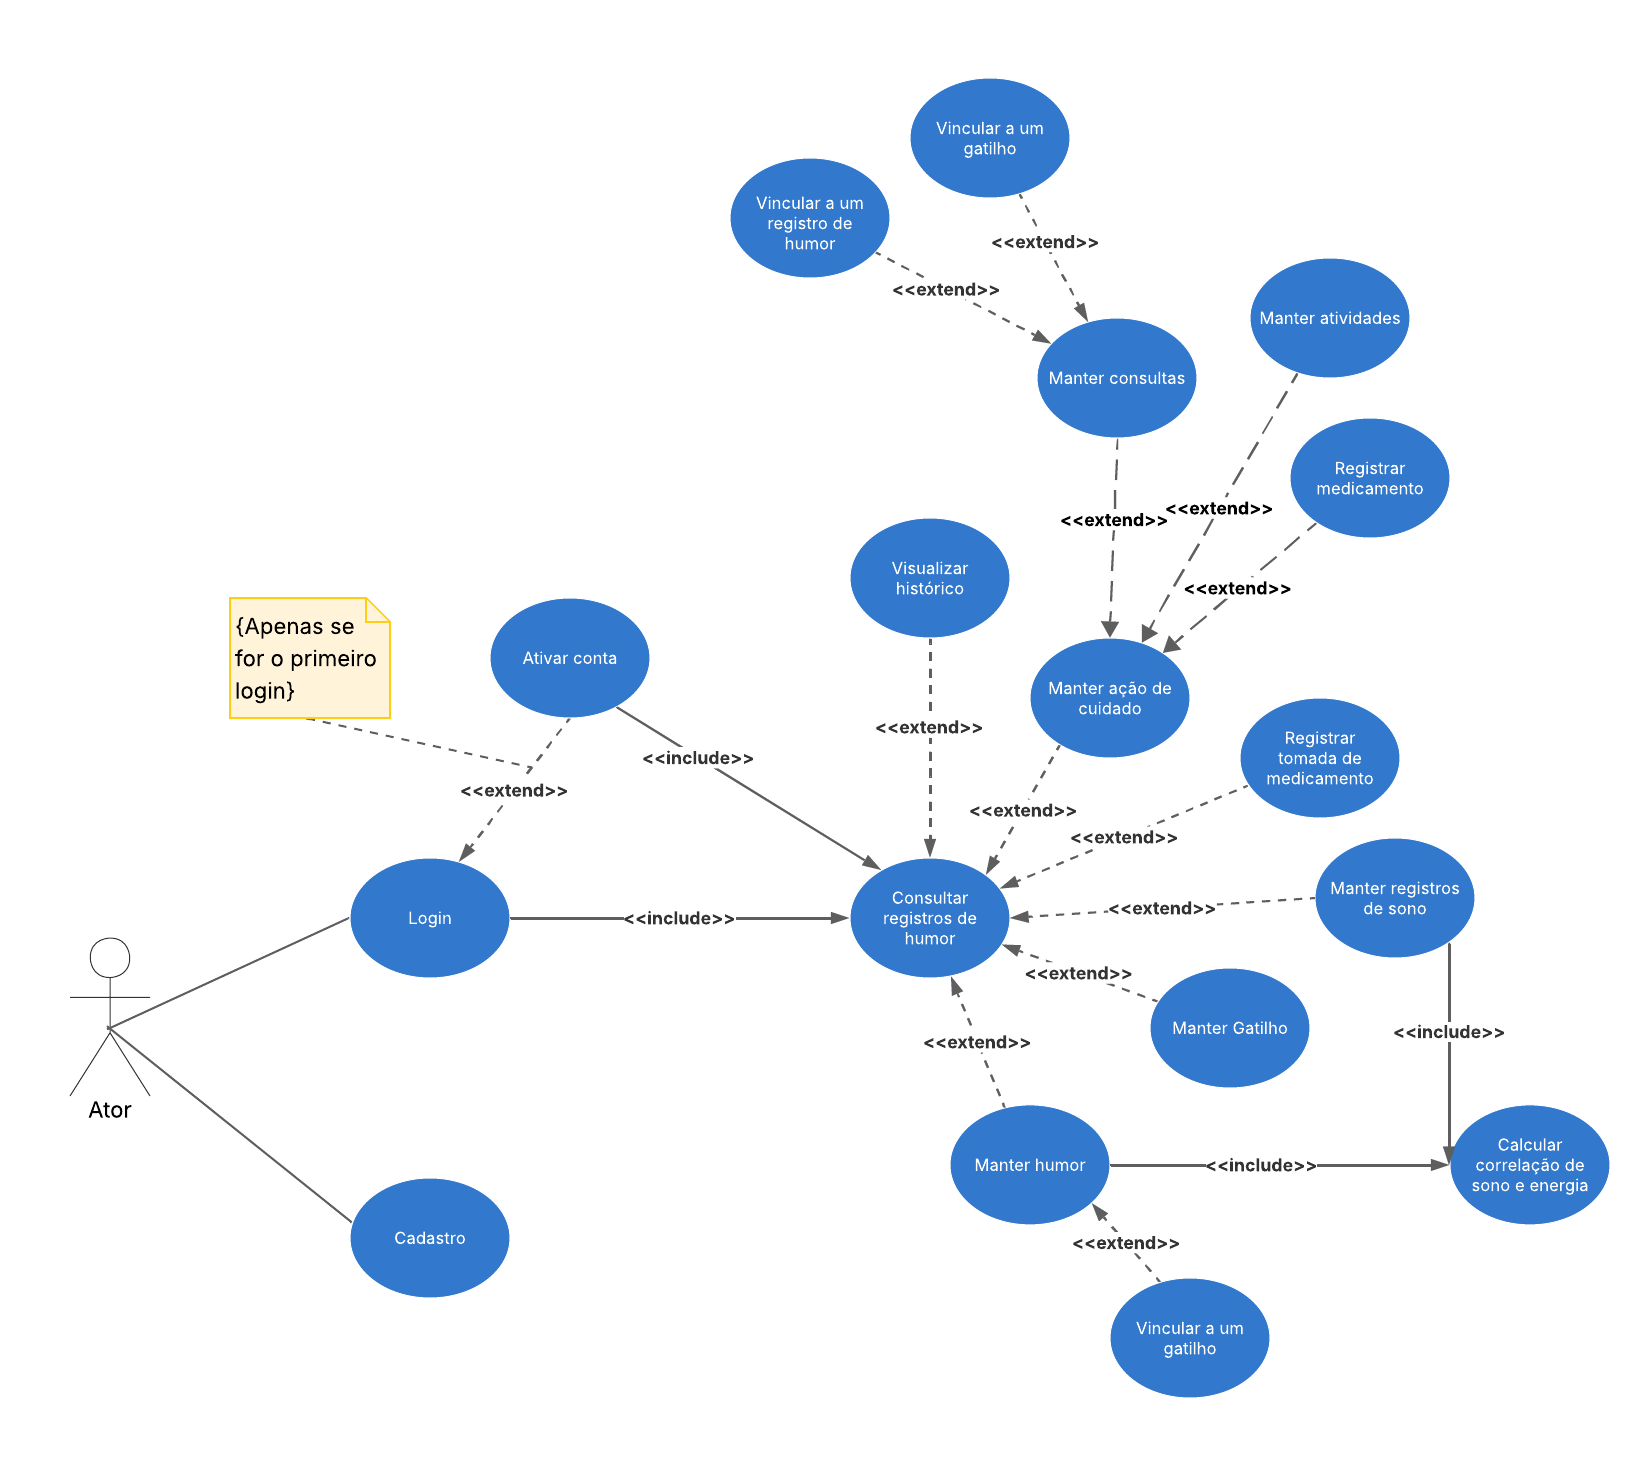
\includegraphics[width=0.9\linewidth]{use-cases.png}
\source{Elaborado pelo autor (2026)}
\end{figure}

Na Figura~\ref{fig:use-cases}, pode-se observar que apenas um ator interage
com o sistema, o próprio usuário final. Também visualiza-se que cada elipse,
se resume a um requisito funcional, e os casos de uso estão interligados por
setas nomeadas com a palavra \textit{``<<extend>>''} que indica conexões onde a
execução de um caso de uso adjacente pode ocorrer dado uma determinada
condição em adição ao caso de uso inicial \cite{ibm:2021}.

Permeando todas as interações no sistema, o caso de uso mais central, o
``Login'', cujo qual estabelece uma base de autenticação, de forma que garante
que apenas usuários autenticados possam interagir com o sistema.

No caso de uso ``Manter Humor'' representa a funcionalidade central do sistema,
permitindo que o usuário registre seu estado emocional ao longo do tempo. Essa
ação ocorre por meio da inserção direta de uma informação de humor, cujo qual o
usuário pode selecionar entre cinco humores ``basais'', além de elementos que
ajudem a compreender, como escalas indicativas dos respectivos níveis de
estresse, ansiedade e quais componentes do humor o usuário identifica com mais
presença. A manutenção do humor no sistema contempla tanto a criação quanto a
edição e a exclusão desses registros.

O caso de uso ``Registrar Intervenção'' contempla o cadastro de estratégias,
práticas ou sugestões que o usuário utiliza ou deseja utilizar para lidar com
oscilações emocionais. As ações de cuidados, podem incluir desde ações
práticas, como caminhar, até técnicas cognitivas ou expressivas, como
atividades criativas, medicamentos utilizados ou atendimentos com profissionais
da área. Essa funcionalidade contribui para que o sistema sirva como uma
central e colabora para construir um registro mais criterioso, visto que o
usuário reconstrói o que aconteceu naquele determinado ponto no tempo.

O caso de uso ``Registrar Gatilho'' visa permitir que o usuário registre
eventos, sejam eles pensamentos, situações, ou estímulos que tenham
influenciado significativamente seu estado emocional. O objetivo é construir um
histórico de causas associadas a variações no humor, de modo a fomentar a
identificação de padrões recorrentes ou específicos. Essa funcionalidade é
especialmente útil para usuários em contextos terapêuticos ou de
autoconhecimento, favorecendo a análise de relações entre circunstâncias
externas e reações internas.

O caso de ``Registro de sono'', permite o usuário, de forma simples, criar no
sistema um registro da quantidade de horas de sono, e adicionar alguma anotação
breve. Esse elemento corrobora com a construção de indicadores, tanto da média
de sono, quanto também de estimular uma correlação entre sono e os níveis de
energia informado em cada humor.

Por fim, o caso de uso ``Vincular humor a um gatilho'' permite ao usuário
estabelecer vínculos entre os gatilhos identificados e os registros de humor,
formando um mapeamento de ação e reação, ou causa e reação. Essa associação
pode servir tanto para consulta futura quanto para, em um futuro, gerar
indicadores. Ao conectar eventos e suas respostas, a funcionalidade fortalece o
papel do sistema como uma ferramenta alinhada com o EMA, gerando assim uma
narrativa emocional diária.

\subsection{Diagrama de Classes}

O diagrama de classes é um dos principais artefatos da UML, responsável por
evidenciar a estrutura estática do sistema, seus atributos, operações e
relacionamentos. Conforme \cite[p. 101]{guedes:2022}: ``O principal enfoque é
permitir a visualização das classes que o sistema e seus respectivos métodos e
atributos''. Dessa forma, esse diagrama constitui a base da modelagem
estrutural que posteriormente será implementada em código.

Sobre o diagrama em si, cada classe possui três partes: título, os atributos,
que representam as características da classe em si, e seus métodos, que são as
operações que o sistema pode operar nos objetos das classes \cite{guedes:2022}. Na
Figura~\ref{fig:classes}, pode-se observar os elementos descritos acima:

\begin{figure}[h]
\centering
\caption{Diagrama de Classes}
\label{fig:classes}
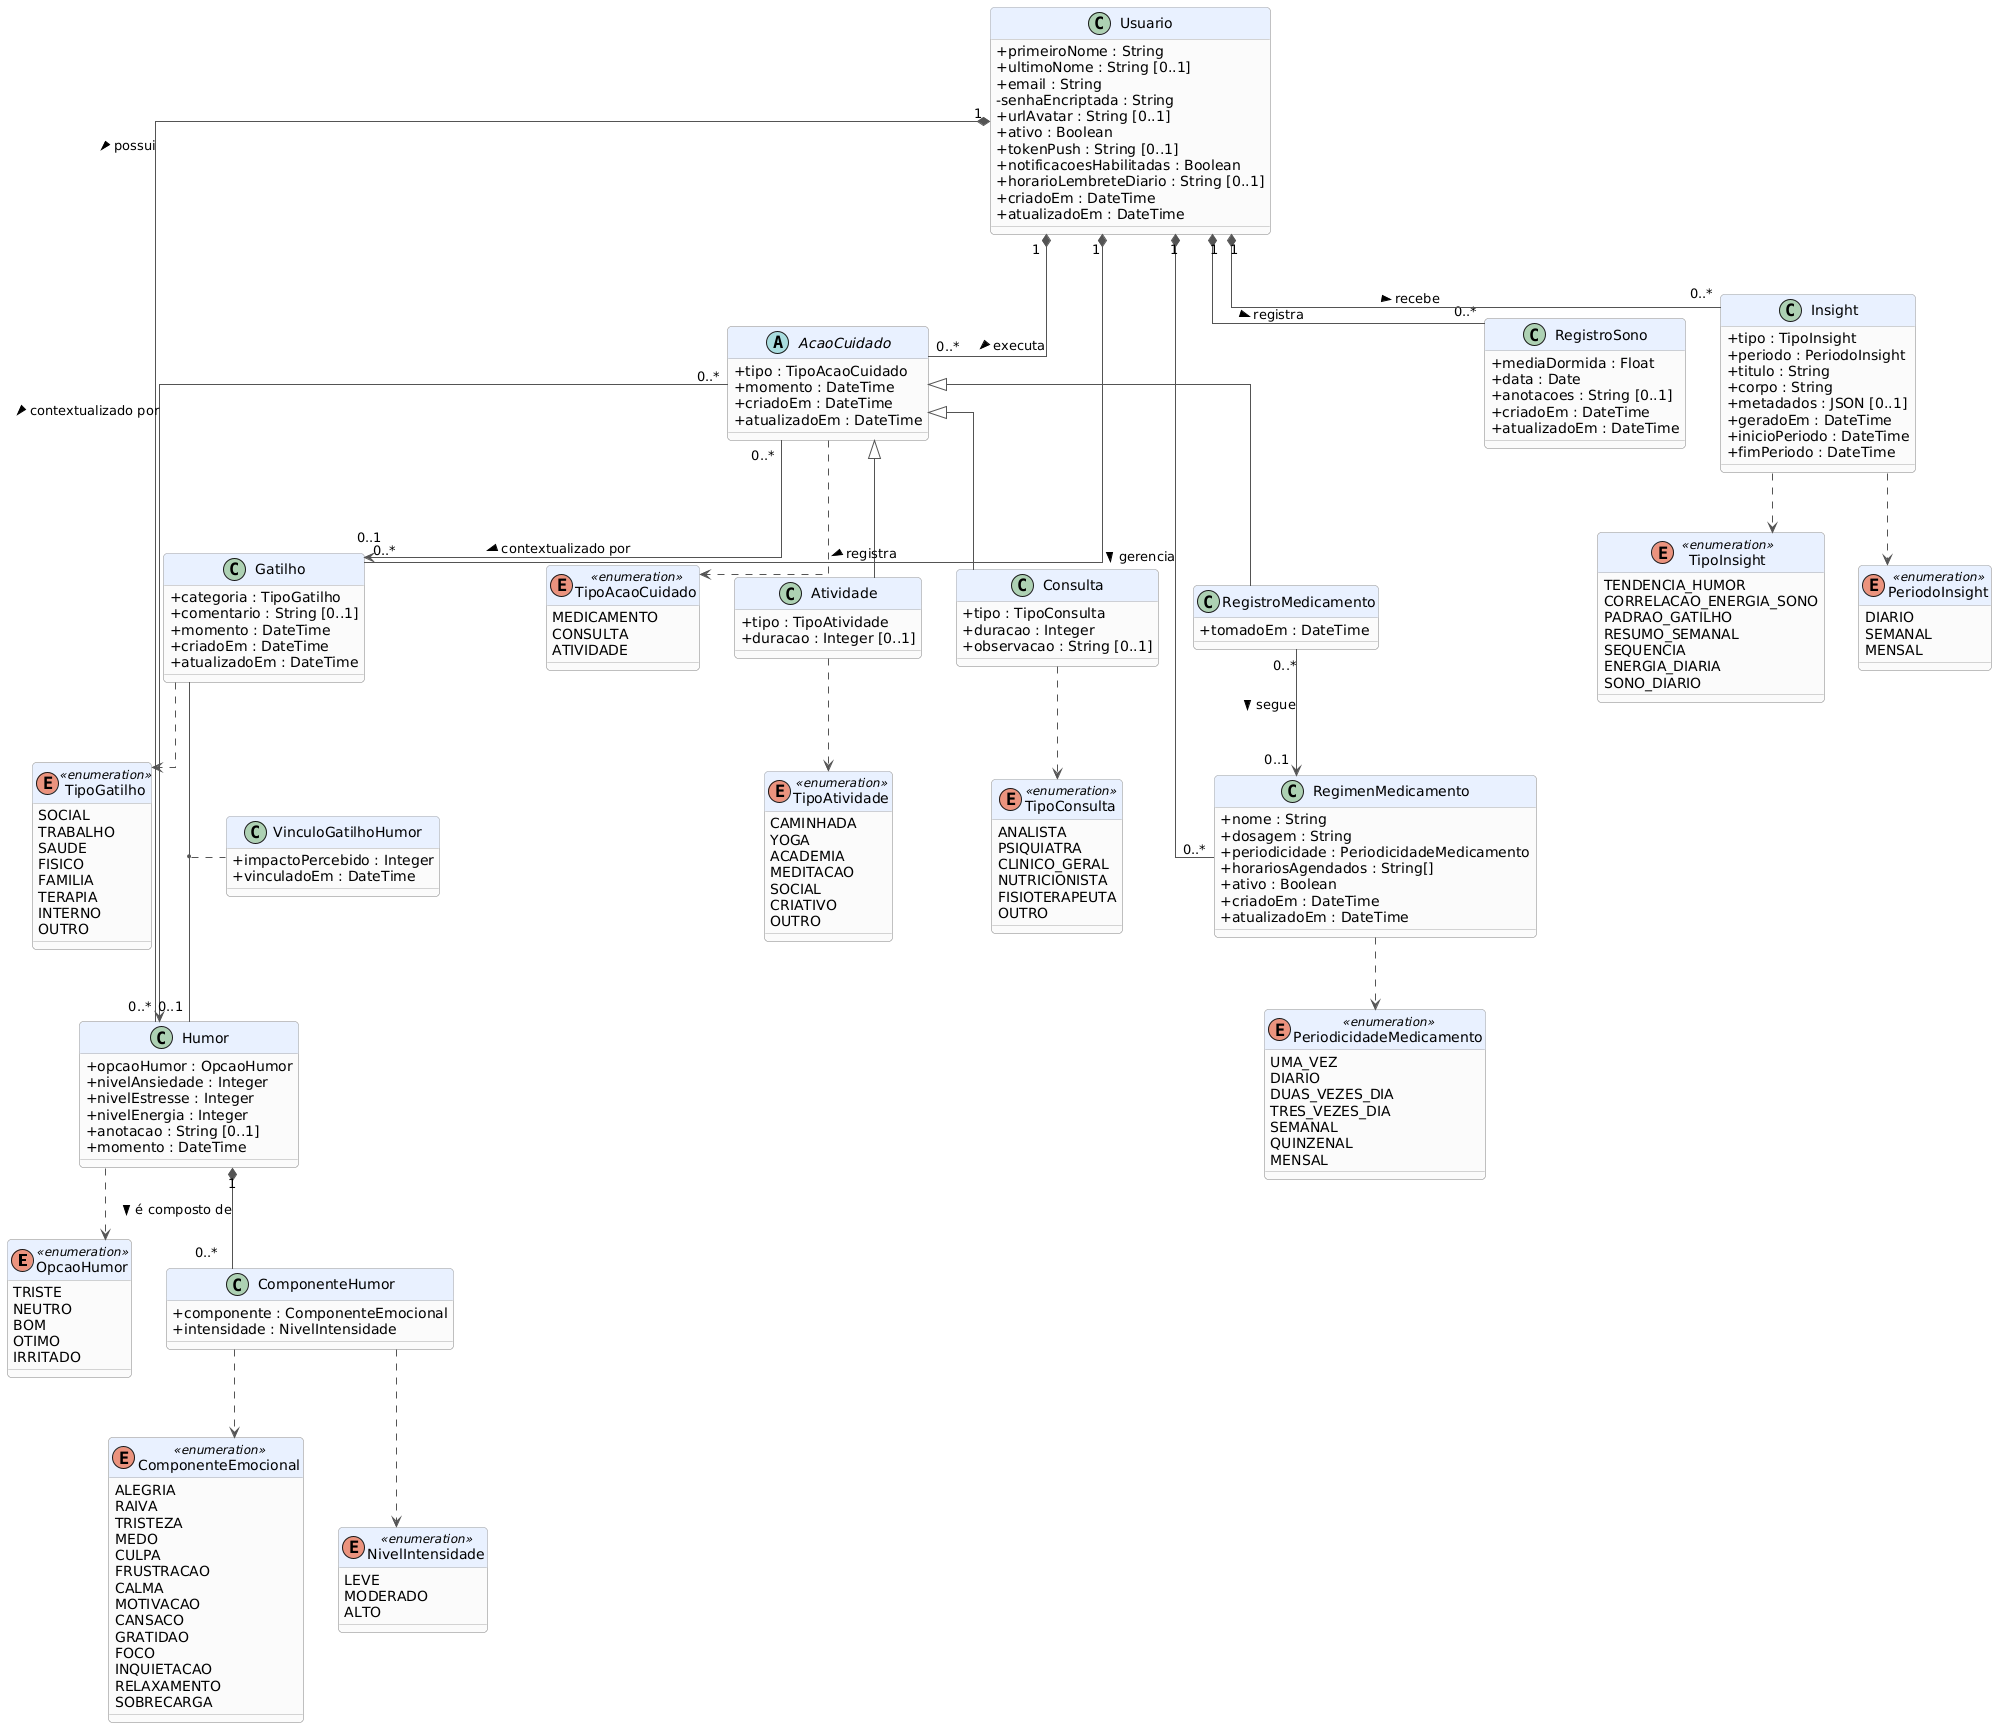
\includegraphics[width=0.9\linewidth]{classes-v2.png}
\source{Elaborado pelo autor (2026)}
\end{figure}

Essa representação apresenta alguns vários elementos importantes. Primeiro, um
acoplamento entre \textit{Usuário} e as demais classes. Isso é natural, e
desejado, considerando que é o único ator. Existe também a separação entre as
entidades como Gatilho, Humor, muito embora exista uma relação de associação
entre elas, através da classe denominada ``VinculoGatilhoHumor'', visto que ela
seria representada por uma tabela auxiliar ligando as duas, aliadas do atributo
de estimativa de impacto.

Necessário destacar aqui que a classe ``AcaoCuidado'' é uma classe abstrata,
representando uma generalização. Essa classe serve como um guarda-chuva para
representar diversos tipos de ações que o usuário pode realizar. O papel dela
aqui se torna guardar elementos em comum entre esses tipos de ações, seus
respectivos vínculos com gatilhos ou humores. A partir dela então, traça-se
outras sub-classes que contem um melhor contexto sobre a atividade em si, por
exemplo, na classe ``Consulta'' guarda-se dados como a duração da consulta, que
tipo de consulta, e potenciais anotações ou comentários em cima da mesma.
Entretanto, uma classe ``RegistroMedicamento'' não precisa guardar mais do que
a relação com qual medicamento e quando ele foi de fato tomado.

Por fim, existe diversos tipos de enumeradores que delimitam exatamente quais
tipos de valores podem ser escolhidos. Esses enumeradores servem também como um
mecanismo de validação, sendo movidos tanto para o próprio banco de dados e
posteriormente sendo implementados como forma de controle em outros pontos como
na API.

Ressalta-se, contudo, que o diagrama não contempla, padrões arquiteturais
complementares, como \textit{Service Layer}, \textit{Repository} e \textit{Data
Access Object (DAO)}, os quais são incorporados na etapa de implementação para
garantir uma separação adequada de responsabilidades e facilitar a manutenção e
escalabilidade do código, conforme as propostas de \citet{Fowler_2013} e
\citet{Gamma:2011}. Esses elementos são importantes, considerando os princípios
de legibilidade, simplicidade e responsabilidades, muitos organizados por
\citet{Martin_2012}, asseguram que o código produzido seja limpo e sustentável.

\chapter{Design}

% TODO: Find citations

As decisões de design do sistema foram fundamentadas tanto na análise dos
aplicativos similares quanto nos resultados do questionário aplicado durante a
etapa de pesquisa. Esses elementos permitiram identificar padrões recorrentes
de interface e compreender as preferências do público-alvo, orientando a
definição da identidade visual, da linguagem adotada e da organização dos
elementos da interface.

A análise dos aplicativos similares revelou uma linguagem visual comum entre as
soluções existentes, caracterizada por interfaces lúdicas, linguagem informal
e, em alguns casos, uso intenso de cores. Paralelamente, os resultados do
questionário indicaram que 37,5\% dos participantes preferem uma comunicação
acolhedora e empática, enquanto 25\% demonstraram preferência por uma linguagem
neutra e objetiva.

O design, no contexto de desenvolvimento de software é um elemento fundamental,
considerando que influencia diretamente a experiência do usuário, na percepção
e assimilação das informações.

Diferentemente da maioria dos aplicativos analisados, optou-se por uma
identidade visual menos lúdica e mais sóbria, reduzindo o uso de ilustrações e
cores saturadas em favor de uma linguagem mais discreta e orientada ao
conteúdo.

\section{Identidade visual}

Identidade visual, neste trabalho, designa o conjunto de decisões gráficas que
conferem ao aplicativo uma aparência reconhecível e consistente: o nome e o
logotipo, a hierarquia visual, a paleta de cores e a tipografia. Esses
elementos constituem a primeira camada de comunicação entre o sistema e o
usuário e materializam as preferências identificadas na etapa de pesquisa ---
em especial a opção por uma linguagem sóbria e acolhedora. Como apontam os
princípios universais de design, a consistência e o reconhecimento desses
elementos reduzem a carga de interpretação e tornam a interface mais previsível
\cite{Lidwell_2011}. As subseções seguintes percorrem cada uma dessas decisões.

\subsection{Nome e Logotipo}

O termo Nexo remete à ideia de conexão, relação e convergência entre
diferentes elementos. Esse conceito dialoga diretamente com a proposta do
projeto, fundamentada na metodologia de Avaliação Ecológica Momentânea (EMA).
Embora seja cada vez mais comum monitorar aspectos isolados da rotina, como
qualidade do sono, nível de atividade física ou uso de medicamentos, essas
informações frequentemente permanecem fragmentadas, dificultando a compreensão
das relações existentes entre elas.

Nesse contexto, o nome Nexo representa a proposta central do sistema: integrar
essas informações e auxiliar o usuário na construção de uma narrativa coerente
sobre seu estado emocional. Em vez de tratar humor, emoções, estresse, energia,
ansiedade, atividades, psicofármacos e consultas como registros independentes,
o aplicativo busca evidenciar como esses fatores se relacionam ao longo do
tempo, favorecendo a identificação de padrões e possíveis associações.

\begin{figure}[H]
\centering
\caption{Logotipo do sistema}
\label{fig:logo}

\includegraphics[width=0.4\linewidth]{logo.png}
\source{Elaborado pelo autor (2026)}
\end{figure}

Assim, tanto o nome quanto o logotipo procuram transmitir a ideia de
convergência, de ``dar a liga'', representando o papel do sistema em conectar
informações dispersas e transformá-las em conhecimento útil para o processo de
autorreflexão.

Para convergir com a pesquisa de tonalidade, e abraçar uma estética
``acolhedora'', o logo tenta fugir de parecer algo mecânico ao usar uma técnica
que simule pinceladas ao invés de linhas retas, simulando também diferenças ou
falhas na pressão utilizada por ter pequenas variações e espaços em branco no
logotipo.

\subsection{Hierarquia visual}

No contexto de interfaces digitais, a hierarquia visual corresponde à
estruturação de elementos de uma tela ou página de forma a narrar e orientar o
usuário com os elementos que são mais significativos e que demandam mais
atenção.

Por meio de repetições de padrões de agrupamento de informações, contraste,
tamanhos, espaçamentos, busca-se reduzir o esforço necessário para encontrar
elementos importantes e quais ações necessitam de maior visibilidade. Segundo
\citet{Lidwell_2011} uma hierarquia visual bem definida, ajuda o usuário a
interpretar rápidamente a interface, reduzindo a carga cognitiva e tornando a
navegação mais intuitiva.

Portanto, com esse foco em mente, produziu-se uma lista pequena de componentes
com visual semelhante, reduzindo o contraste entre esses mesmo elementos, o que
ajuda justamente a gerar uma sensação de consistência e previsibilidade entre
telas e elementos gráficos.

A estrutura da aplicação pode ser resumida em cinco componentes fundamentais:
cartões (\textit{cards}), botões de ação, \textit{chips} para categorização de
informações, campos de formulário e indicadores em escala (\textit{sliders}).
Esses componentes aparecem de maneira recorrente em praticamente todas as telas
do sistema, permitindo que o usuário reconheça rapidamente sua função sem
necessidade de reaprendizado.

Portanto, a organização de telas geralmente se dá nesses mesmos parâmetros, em
que toda tela é dividida em seções, compostas de um cabeçalho, seguido dos
respectivos elementos de interação. Posteriormente, a utilização de cartões,
ajuda a reforçar esse foco visual, agrupando elementos que são interativos e/ou
que necessitam interação e/ou atenção.

\subsection{Paleta de Cores}

Como discutido anteriormente, a definição da paleta de cores buscou equilibrar
dois objetivos identificados durante a fase de pesquisa, transmitir uma
identidade visual acolhedora, porém evitando excessos de cores e informações
lúdicas. Portanto, para buscar esses pilares, optou-se por usar uma escolha de
cores mais neutras e sóbrias, focando em tons de branco, cinza e preto, de
forma a permitir que o conteúdo regstrado pelo usuário seja o maior foco de
destaque.

\begin{figure}[h]
  \centering
  \caption{Paleta de cores}
  \label{fig:palette}
  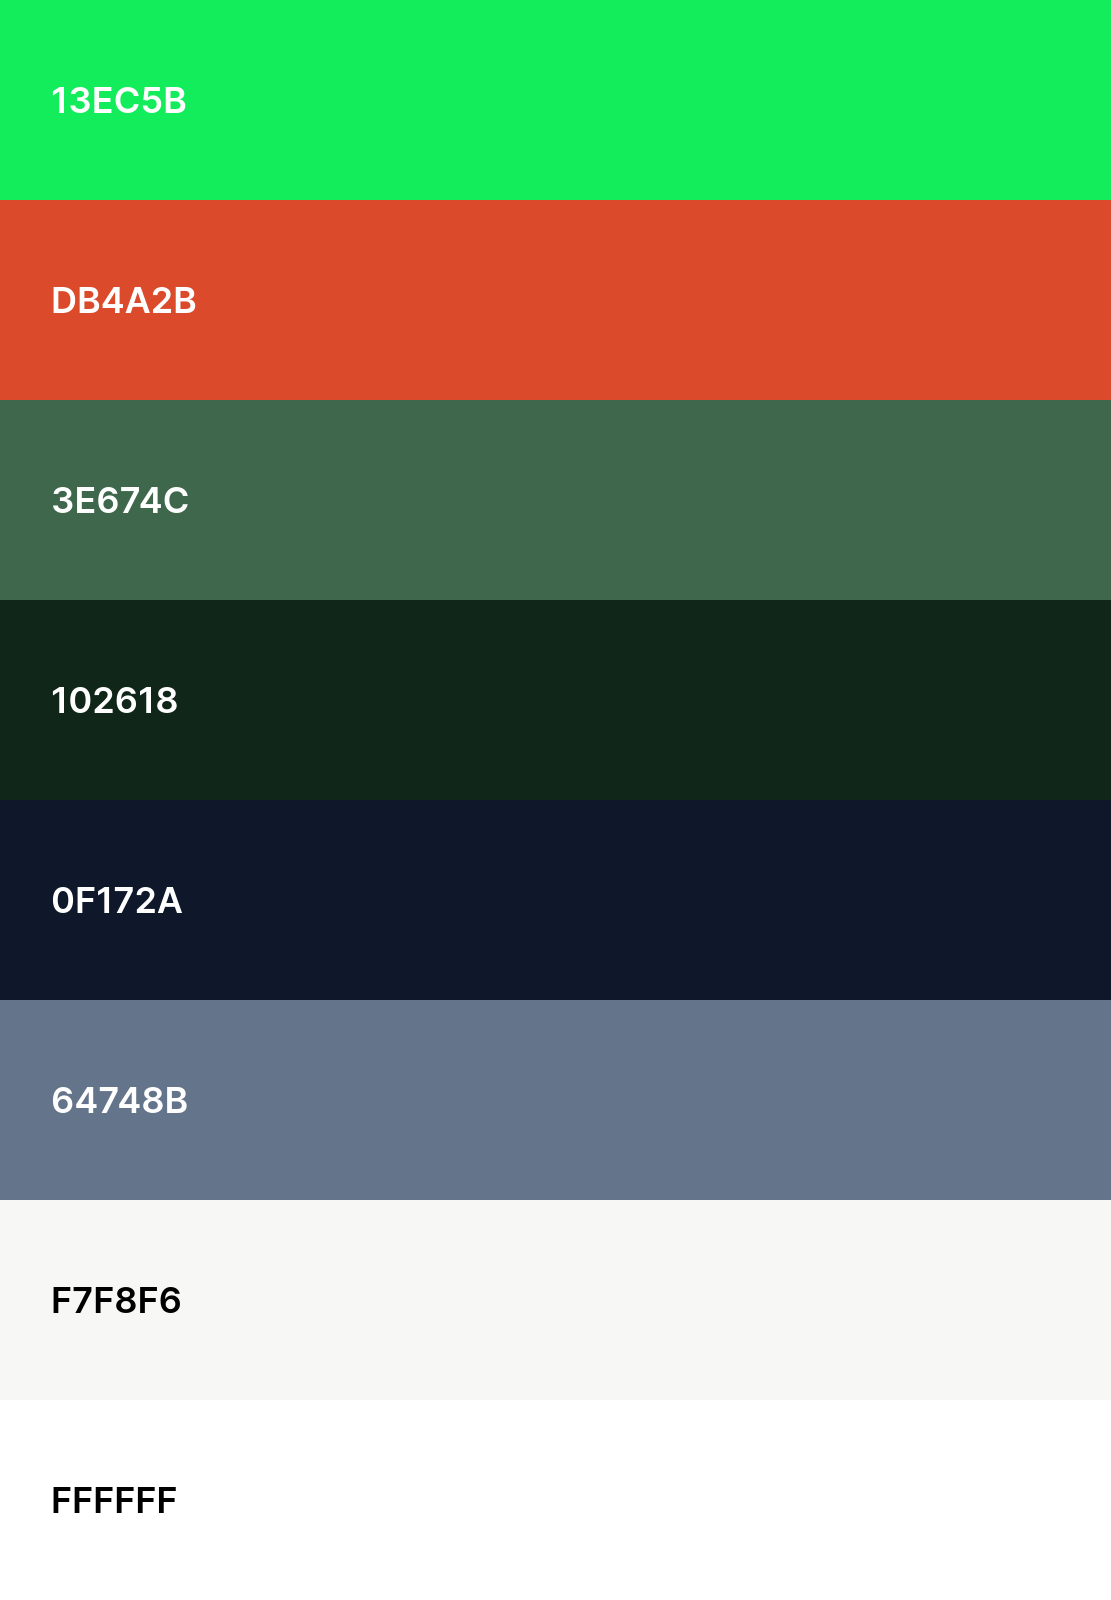
\includegraphics[width=10cm, height=8cm, keepaspectratio]{pallete-small.png}
  \source{Elaborado pelo autor (2026)}
\end{figure}

% Hack
\newpage

Contudo, para elementos que necessitam de uma maior atenção, ou elementos de
interação, como botões de ações primárias, adotou-se uma escolha mais rádical,
um tom de verde forte, que busca criar exatamente a sensação de destaque
imediato. Além disso, o verde geralmente está associado como uma cor que
transmite uma sensação de vitalidade, força, natureza, bem-estar e afins. Como
mencionado anteriormente, limitou-se a utilização para indicadores, componentes
de interação e elementos que representam progresso ou confirmação.

Por fim, foi escolhido outras cores pasteis para ajudar a destacar elementos
como sentimento e emoções, indicadores para cada tipo de registro gerado no
sistema, de forma mínima e não intrusiva.

\subsection{Tipografia}

A tipografia constitui um dos principais elementos responsáveis pela
legibilidade em interfaces digitais. Segundo o Material Design
\cite{Google_2021}, a escolha adequada da fonte influencia diretamente a
velocidade de leitura, a organização da informação e a percepção geral de
qualidade da interface. Em aplicações móveis, onde o espaço disponível é
reduzido, a clareza tipográfica torna-se ainda mais importante.

\begin{figure}[h]
  \centering
  \caption{Referência da fonte Inter}
  \label{fig:ref-inter}
  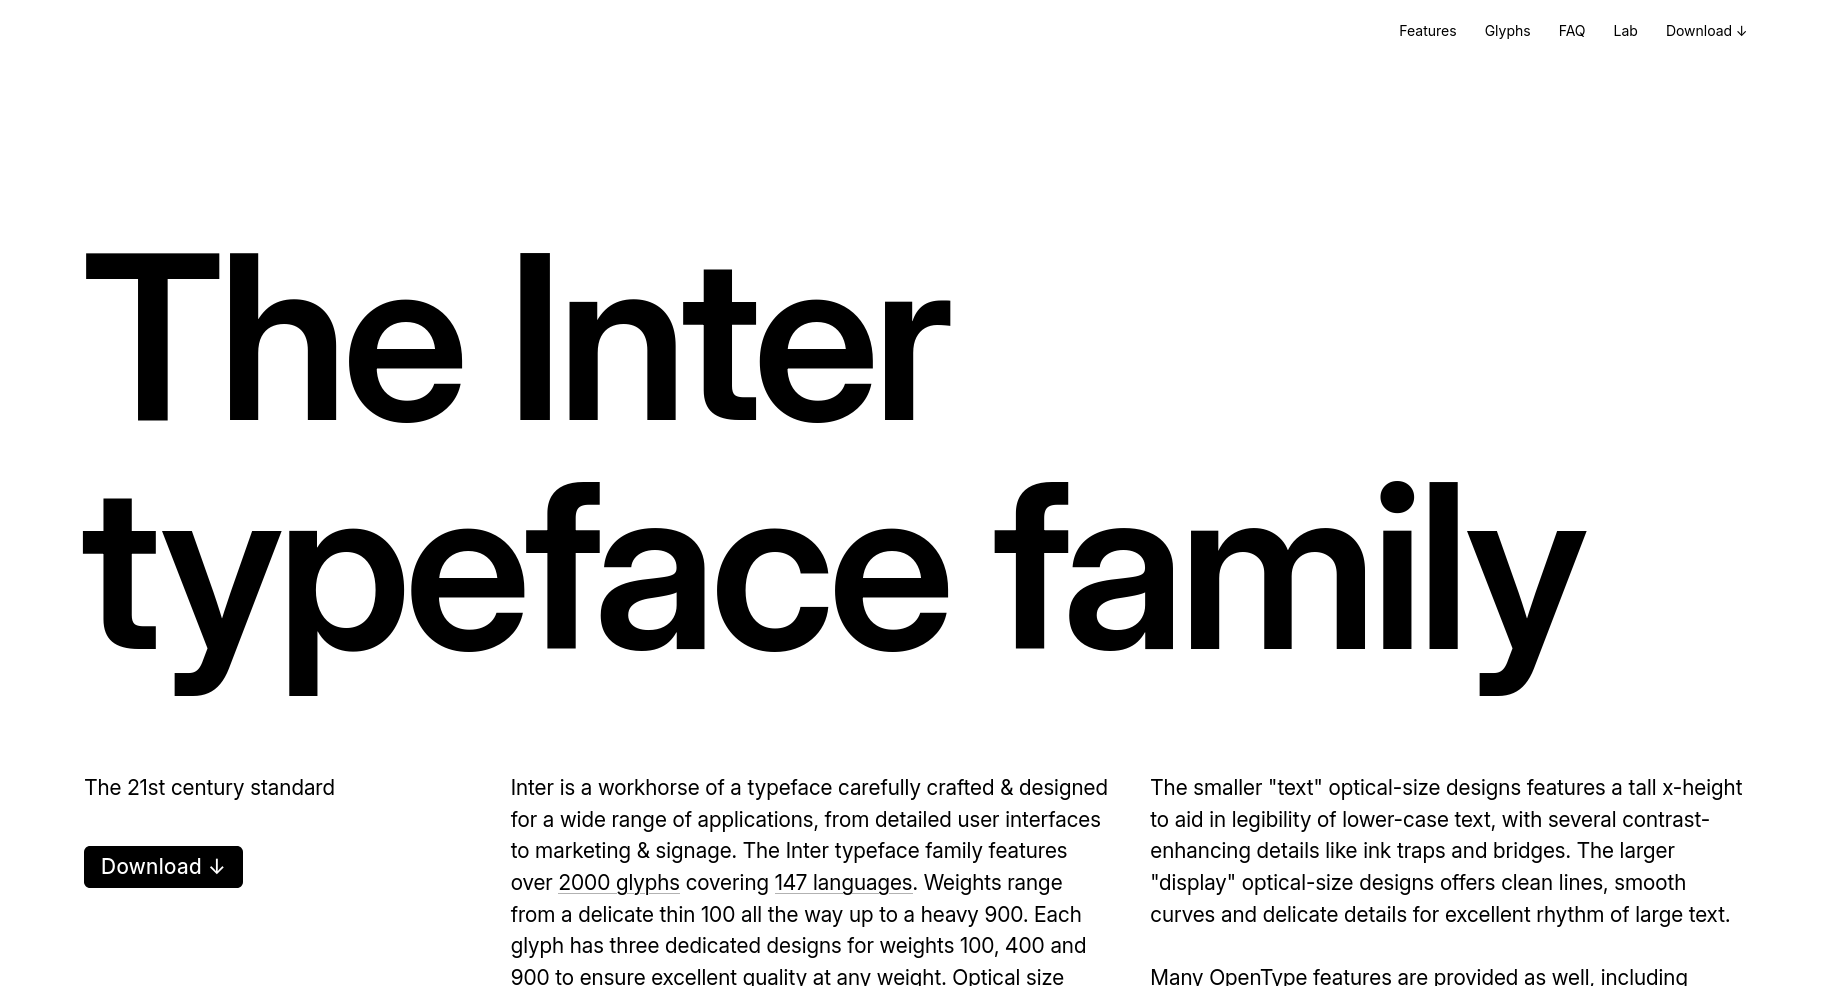
\includegraphics[width=10cm, height=8cm, keepaspectratio]{ref-inter.png}
  \source{Site da página da fonte Inter (2026)}
\end{figure}

Considerando esses aspectos, optou-se pela utilização da fonte Inter,
desenvolvida por Rasmus Andersson especificamente para ambientes digitais. A
família tipográfica foi projetada para manter elevada legibilidade em
diferentes tamanhos de tela, apresentando boa diferenciação entre caracteres e
excelente renderização em sistemas operacionais modernos \cite{Andersson_2016}.

A hierarquia tipográfica do sistema foi construída a partir de poucas variações
de tamanho e peso da fonte. Títulos utilizam maior peso tipográfico para
estabelecer prioridade visual, enquanto textos informativos e descrições
empregam pesos mais leves, mantendo consistência em toda a aplicação. Essa
padronização reduz a quantidade de estímulos visuais simultâneos e facilita a
identificação das informações mais relevantes em cada tela.

Além da legibilidade, a escolha da Inter também contribui para reforçar a
identidade moderna e funcional proposta pelo aplicativo. Por ser amplamente
utilizada em plataformas digitais e ferramentas de interface, como o Figma, a
fonte transmite familiaridade ao usuário e mantém consistência com os padrões
contemporâneos de design de interfaces.

\section{Estrutura}

Por estrutura entende-se a organização das telas e da navegação do aplicativo:
o que cada tela contém, em que ordem os elementos se apresentam e como o
usuário se desloca entre elas. No Nexo, essa organização repousa sobre dois
alicerces: uma navegação por abas que divide o sistema em cinco áreas ---
Histórico, Jornada, Novo, Ações de Cuidado e Configurações --- e a composição
das telas por cartões reutilizáveis, descritos na seção anterior. Esta seção
apresenta como essa estrutura foi planejada e mapeada antes da aplicação da
identidade visual definitiva.

\subsection{Organização da navegação}

A navegação do Nexo é organizada em cinco áreas, acessíveis por uma barra de
abas inferior: ``Histórico'', ``Jornada'', ``Novo'', ``Ações de Cuidado'' e
``Configurações''. A divisão separa as superfícies de consulta --- Histórico e
Jornada, que apresentam registros e indicadores já consolidados --- do ponto de
entrada rápido para o registro de humor, a aba Novo. As ações de cuidado, por
reunirem modalidades distintas (medicamentos, consultas e atividades), são
agrupadas em um único hub, evitando que cada tipo ocupe uma entrada própria na
navegação.

\subsection{Consolidação de registros no Histórico}

Uma decisão estrutural relevante foi consolidar os registros em uma única linha
do tempo. Em vez de listas separadas para humor, sono, gatilhos e ações de
cuidado, a tela de Histórico combina os quatro tipos em uma sequência
cronológica única, agrupada por dia, por meio de um componente de mapeamento
que normaliza cada recurso em um formato comum, descrito no Capítulo
\ref{sec:history-analysis}. A motivação decorre da própria metodologia EMA:
aproximar visualmente eventos relacionados --- como um gatilho registrado
minutos antes de um humor --- permite reconstruir uma narrativa do dia em vez
de fragmentar o contexto em telas distintas.

\subsection{Wireframes}

\textit{Wireframes} são representações simplificadas de uma interface, focadas
na estrutura e na disposição dos elementos, sem se preocupar ainda com
componentes visuais definitivos, cores ou tipografia. Essa camada de abstração
permite válidar rapidamente o que cada tela precisa conter e como o usuário
navegaria entre elas, antes de investir tempo no design em alta fidelidade, no
qual esses elementos visuais são então aplicados. Quando elementos
clicáveis/interativos são adicionados aos \textit{wireframes}, eles também
podem se tornar protótipos, usados para modelar e avaliar o fluxo de navegação
entre as telas.

No desenvolvimento do aplicativo, essa prática foi usada para mapear as telas
existentes e definir quais elementos cada uma apresentaria, como exemplifica a
tela inicial na Figura \ref{fig:wireframe-initial}:

\begin{figure}[h]
  \centering
  \caption{\textit{Wireframe} da tela inicial}
  \label{fig:wireframe-initial}
  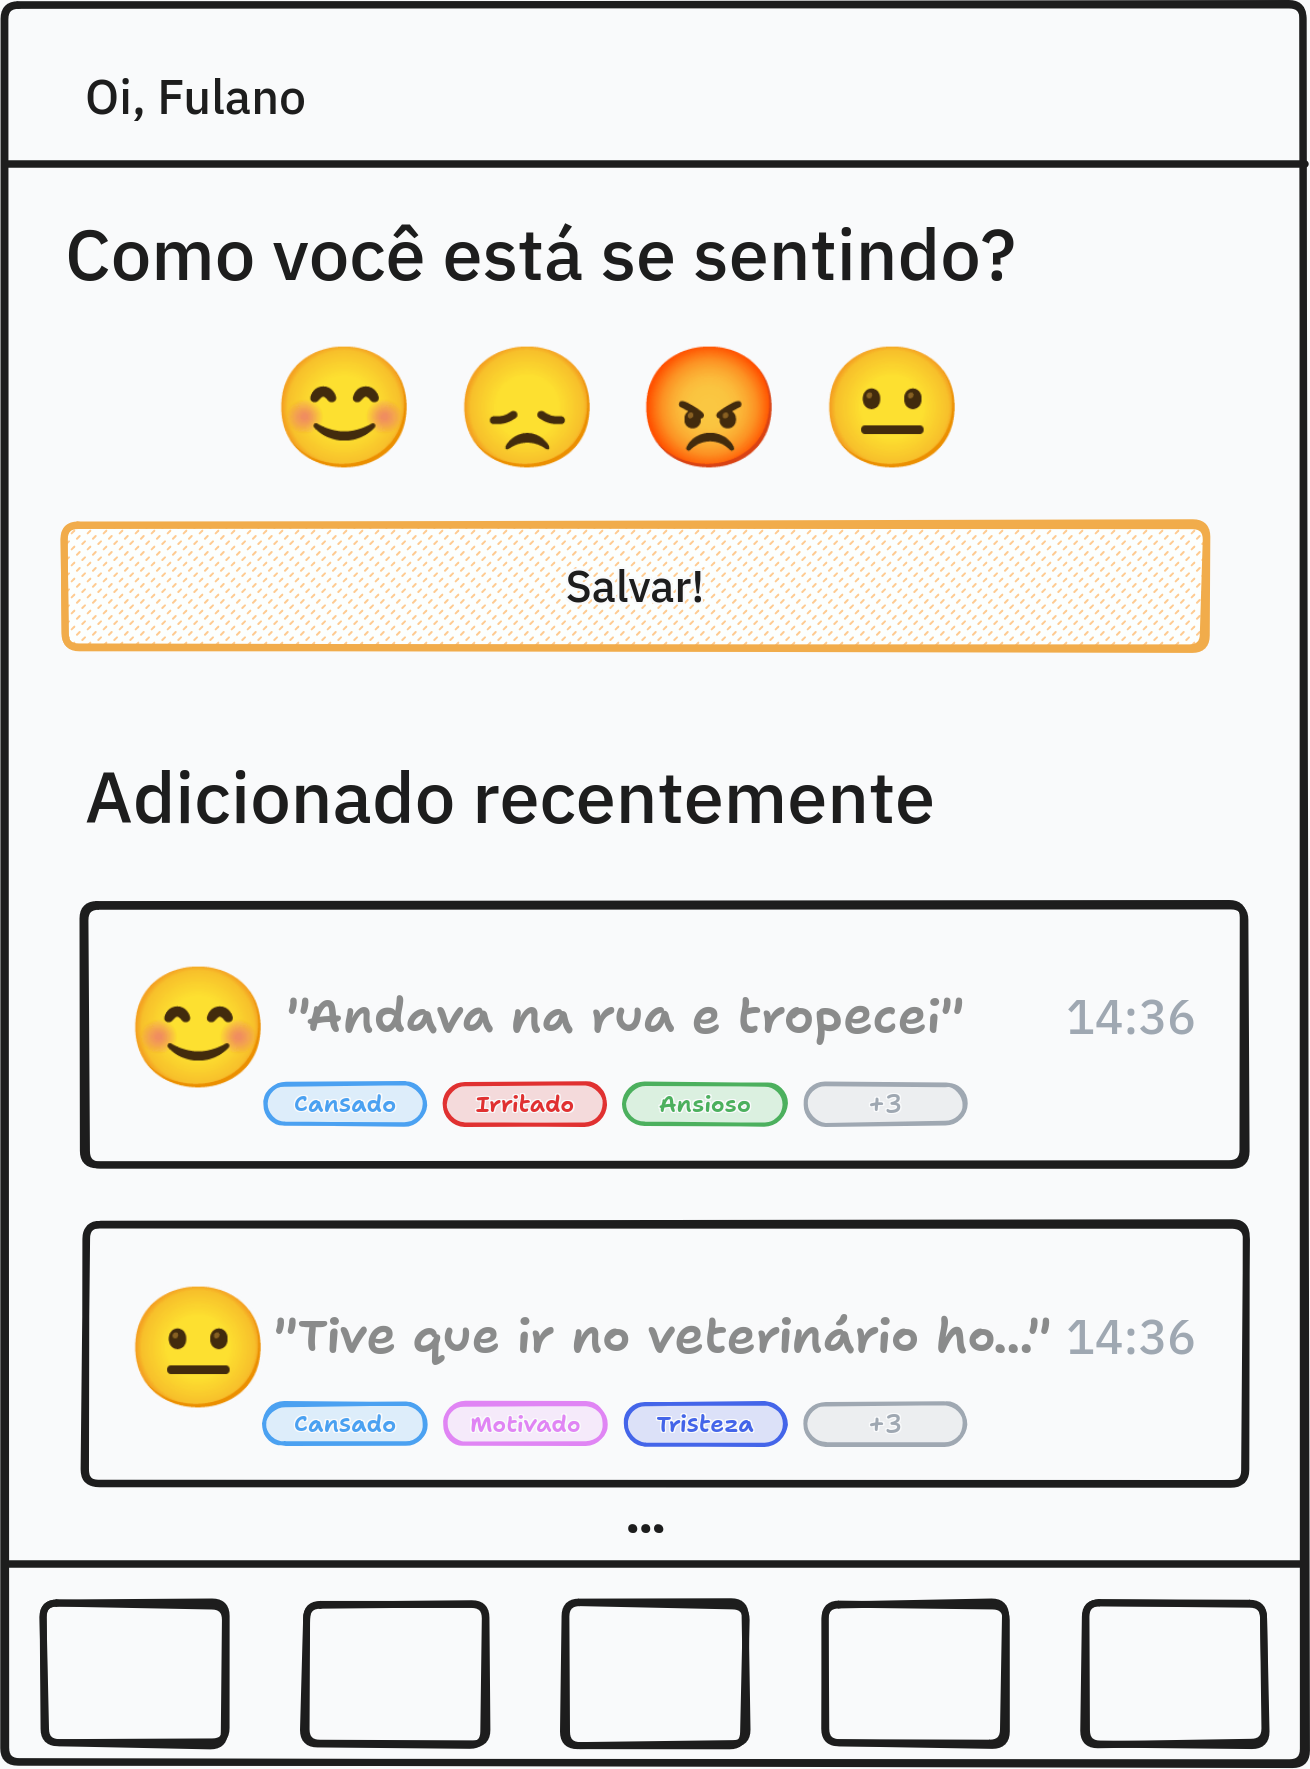
\includegraphics[width=10cm, height=8cm, keepaspectratio]{wireframe-initial.png}
  \source{Elaborado pelo autor (2026)}
\end{figure}

Alguns elementos podem ser notados nessa tela, como a presença de
\textit{cards} e emojis, utilizados para criar destaque visual. A escolha de
emojis foi inspirada pelo aplicativo analisado no
Capítulo~\ref{chapter:methodologies}, DailyBeans que utiliza ícones para cada
tipo de emoção. Portanto, a escolha de emojis se dá como uma saída rápida e
fácil, visto que não demanda conhecimentos de íconografia.

Um segundo \textit{wireframe}, apresentado na Figura
\ref{fig:wireframe-insights}, mostra uma proposta inicial para a tela de
Indicadores. Nessa versão inicial, o usuário selecionava, por meio de um menu
suspenso, (``Flutuação de:''), qual indicador desejava visualizar, sendo os
dados apresentados em um gráfico de linha que representava a flutuação dos
níveis informados de um humor (``Energia'', ``Ansiedade'' e/ou ``Estresse''),
além de seções para gatilhos frequentes e um indicador de estabilidade de
humor.

\begin{figure}[H]
  \centering
  \caption{\textit{Wireframe} da tela de indicadores}
  \label{fig:wireframe-insights}
  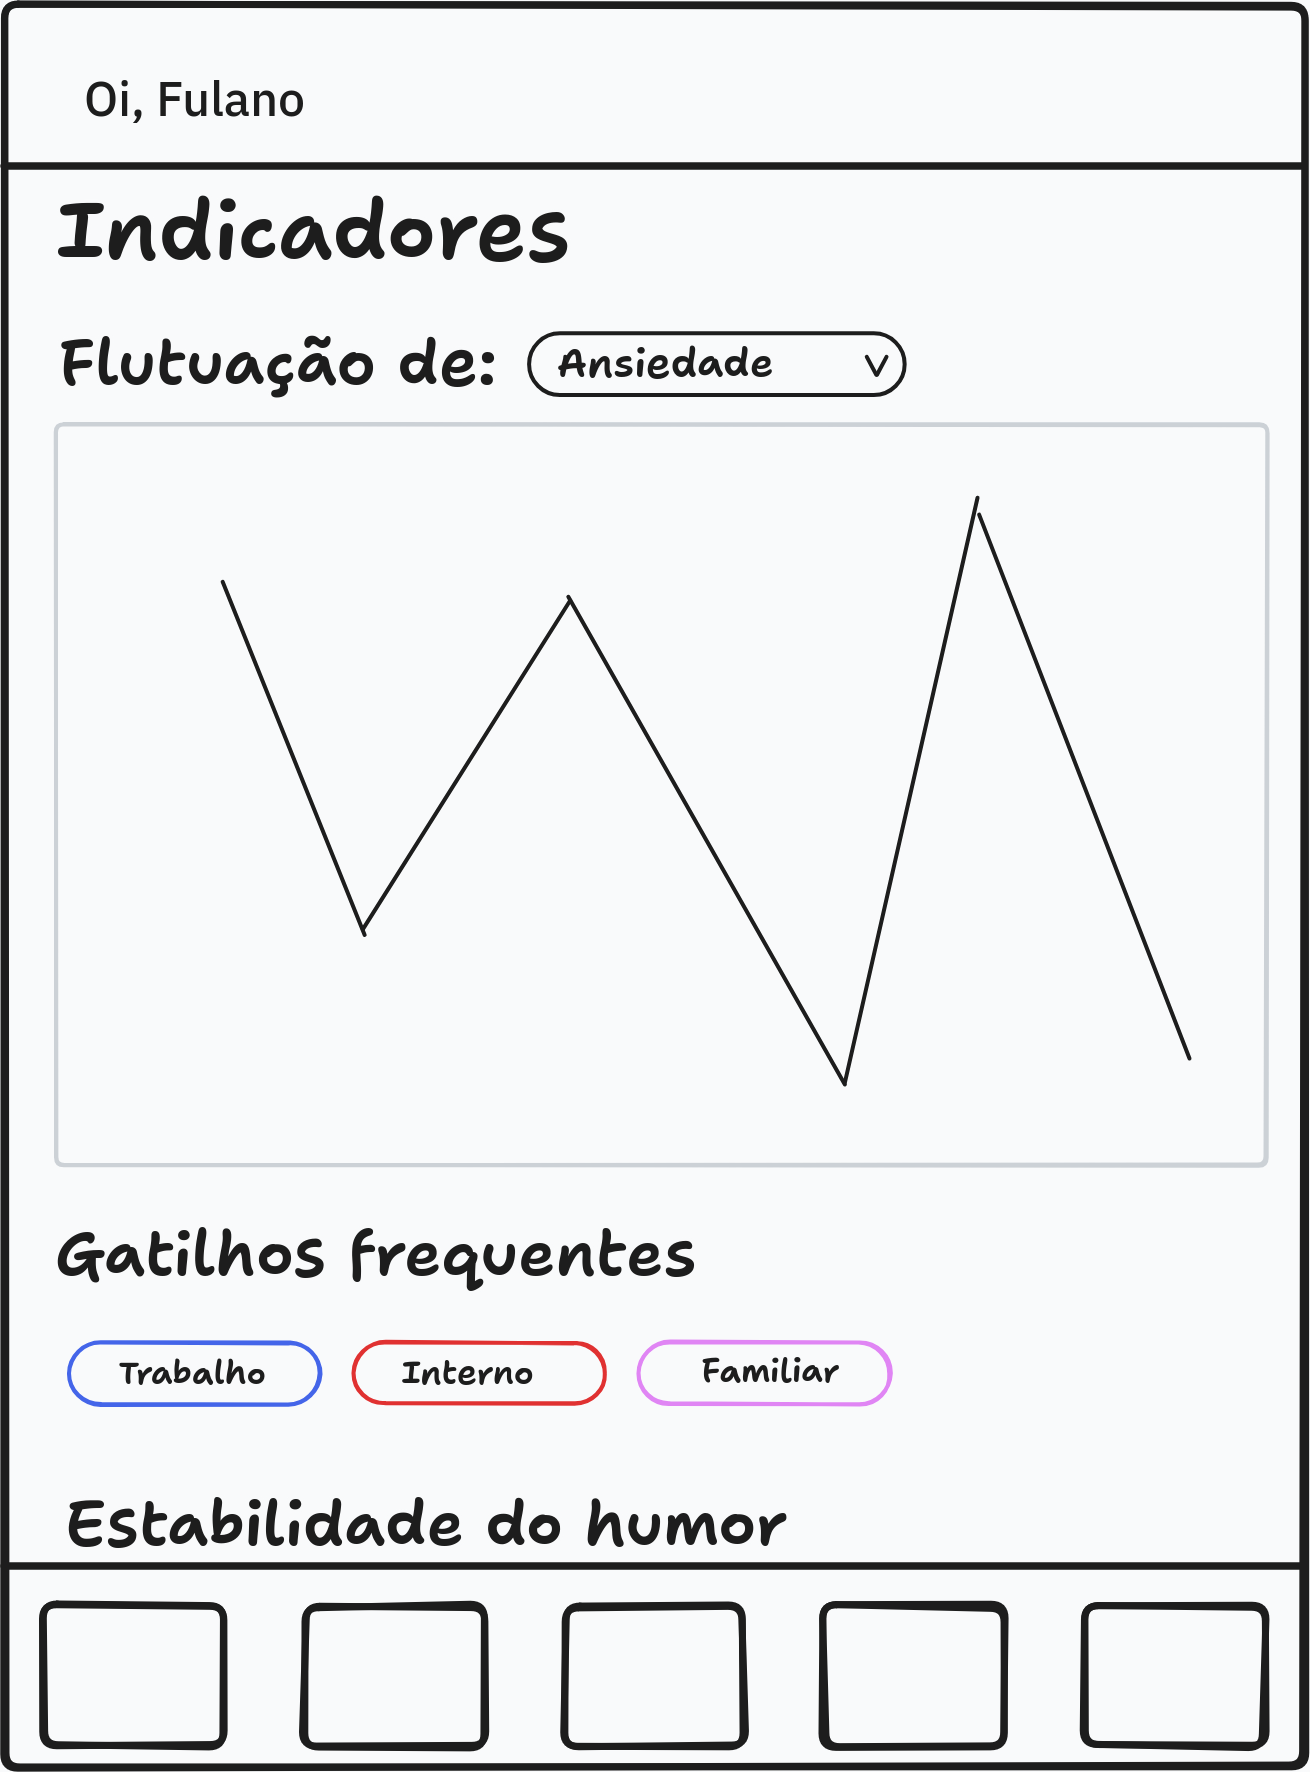
\includegraphics[width=10cm, height=8cm, keepaspectratio]{wireframe-insights.png}
  \source{Elaborado pelo autor (2026)}
\end{figure}

Essa abordagem, contudo, foi descartada na versão final do aplicativo: o
gráfico com seletor de tipo de indicador foi removido, e a tela foi repaginada
para simplificar usando três tipos de indicadores automaticamente cálculados
pelo sistema, conforme detalhado no Capítulo~\ref{sec:insights}.

\chapter{Tecnologias}

Este capítulo apresenta as principais tecnologias empregadas no desenvolvimento
do aplicativo, organizadas de acordo com a camada da arquitetura em que atuam:
\textit{front-end}, \textit{back-end} e infraestrutura/persistência de dados.

\section{Front-end}

O termo \textit{frontend} refere-se à camada de um sistema responsável pela
interação direta com o usuário: a interface visual, a lógica de apresentação e
o processamento que ocorre no dispositivo do próprio usuário, seja um navegador
ou, como no caso do Nexo, um aplicativo móvel, conforme
~\citet{sommerville:2010}. É o frontend que renderiza telas, captura entradas
do usuário (como toques e formulários) e comunica-se com o \textit{backend}
através de requisições de rede, geralmente utilizando APIs. No caso do Nexo,
essa camada é implementada com \textit{React Native} e Expo, permitindo que a
mesma base de código seja compilada tanto para Android utilizando bibliotecas
em \textit{TypeScript}.

\subsection{React Native}

React Native é um \textit{framework} de código aberto, mantido pela Meta, que
permite o desenvolvimento de aplicativos móveis multiplataforma a partir de
uma única base de código escrita em JavaScript/TypeScript, utilizando
componentes que são traduzidos para elementos nativos tanto no iOS quanto no
Android \citep{reactnative:2026}.

A escolha do React Native se justifica pelo escopo reduzido da equipe de
desenvolvimento (um único desenvolvedor) e facilidade de conhecimento e
manutenção, sem trazer, para este projeto, benefícios que justifiquem esse
custo adicional. Além disso, o ecossistema maduro do React Native oferece
ampla disponibilidade de bibliotecas para funcionalidades já previstas no
aplicativo, como notificações locais e gráficos.

\subsection{Zustand}

Zustand é uma biblioteca leve de gerenciamento de estado para aplicações
React e React Native, que dispensa a estrutura verbosa de \textit{providers}
e \textit{reducers} tipicamente associada a bibliotecas como Redux
\citep{zustand:2026}.

Ela foi escolhida para gerenciar o estado efêmero da aplicação (por exemplo,
dados de formulários em preenchimento ou estados de navegação temporários)
por sua API minimalista e baixo \textit{overhead} de configuração, adequada a um
projeto de escopo individual em que a complexidade adicional de soluções
mais robustas de gerenciamento de estado não se justifica.

\section{Back-end}

Já o termo \textit{backend} refere-se à camada de um sistema que processa a
lógica de negócio, gerencia o acesso e a persistência de dados, e expõe essa
funcionalidade a clientes (como o frontend) através de uma interface bem
definida, tipicamente uma API HTTP \cite{Fowler_2013}. O \textit{backend} é
responsável por validar dados recebidos, aplicar regras de negócio, autenticar
usuários, e coordenar o acesso ao banco de dados e a outros serviços
auxiliares. No caso do Nexo, essa camada é implementada em Node.js com o
framework \textit{Express}, seguindo uma arquitetura em camadas (\textit{Route}
$\rightarrow$ \textit{Controller} $\rightarrow$ \textit{Service} $\rightarrow$
Prisma) que separa as responsabilidades de validação, lógica de negócio e
acesso a dados.

\subsection{Express.js}

Express.js é um \textit{framework} minimalista para aplicações web em
Node.js, amplamente utilizado para a construção de APIs \textit{REST},
oferecendo uma camada fina de abstração sobre o roteamento de requisições HTTP e
\textit{middlewares} \citep{express:2026}.

Sua adoção se deve à simplicidade e à flexibilidade não opinativa do
\textit{framework}, que permite estruturar a API de acordo com as
necessidades específicas do projeto, sem impor convenções rígidas de
arquitetura, além de sua ampla documentação e maturidade no ecossistema
Node.js.

\subsection{Zod}

Zod é uma biblioteca de validação e definição de esquemas de dados para
TypeScript, que permite declarar formatos esperados de entrada (como corpos
de requisição) e inferir automaticamente os tipos estáticos correspondentes
\citep{zod:2026}.

Zod foi escolhido para validar os dados recebidos pela API antes de seu
processamento, garantindo que registros de humor, sono e demais entradas do
usuário estejam em conformidade com o formato esperado. A inferência
automática de tipos a partir dos esquemas evita a duplicação de definições de
tipo entre a camada de validação e o restante do código TypeScript do
back-end.

\begin{lstlisting}[language=typescript, caption={Validação e Inferência usando Zod}, label={lst:zod-inference}]
import {
  BaseMoodOption,
  MoodComponentOption,
  IntensityLevel
} from '@prisma/client';

export const MoodComponentSchema = z.object({
  component: z.nativeEnum(MoodComponentOption),
  intensity: z.nativeEnum(IntensityLevel)
});

export const CreateMoodSchema = z.object({
  annotation: z.string().optional(),
  moment: z.coerce.date(),
  selectedMood: z.nativeEnum(BaseMoodOption),
  anxietyLevel: z.number().int().min(0).max(10),
  stressLevel: z.number().int().min(0).max(10),
  energyLevel: z.number().int().min(0).max(10),
  moodComponents: z.array(MoodComponentSchema).min(1)
});

export type CreateMoodInput = z.infer<typeof CreateMoodSchema>;
\end{lstlisting}

\sourcecode{Elaborado pelo autor (2026)}

Aqui, é possível observar alguns elementos, como a extração direta dos
\textit{enums} mapeados pelo Prisma, citado anteriormente nas linhas 1--5. Em
seguida, são criados os \textit{schemas} de validação: um valida os componentes
de humor de forma aninhada dentro do objeto recebido, e o outro valida os dados
do próprio registro --- os níveis aceitos de ansiedade, estresse e energia; a
conversão do campo \texttt{moment} para um objeto de data a partir da entrada
recebida; a exigência de ao menos um componente de humor selecionado; entre
outros. Por fim, esses dados são exportados como um \textit{type} do
TypeScript, usado pelo compilador para a verificação estática de tipos no
restante do back-end.

\subsection{Valkey e BullMQ}

Valkey é um banco de dados em memória, do tipo chave-valor, criado como
\textit{fork} de código aberto do Redis, mantido sob a governança da Linux
Foundation \citep{valkey:2026}. BullMQ é uma biblioteca para gerenciamento de
filas de tarefas em Node.js, construída sobre bancos de dados compatíveis com
o protocolo Redis \citep{bullmq:2026}.

A combinação das duas ferramentas foi adotada para o processamento paralelo
e assíncrono de tarefas que não precisam bloquear a resposta imediata da API,
como o disparo de notificações programadas e o processamento de indicadores
a partir do histórico de registros do usuário. A escolha do Valkey em
específico, e não do Redis diretamente, se deve à mudança de licenciamento do
Redis em 2024, que passou a restringir certos usos comerciais; o Valkey
mantém compatibilidade total de protocolo, permanecendo sob licença
permissiva de código aberto.

\section{Infraestrutura e Persistência de Dados}

A camada de \textit{infraestrutura e persistência} de um sistema abrange os
componentes responsáveis por armazenar e gerenciar os dados de forma durável,
bem como os serviços auxiliares que sustentam o funcionamento da aplicação em
produção \cite{Fowler_2013}. O elemento central dessa camada costuma ser o
sistema de gerenciamento de banco de dados (SGBD), responsável por garantir a
integridade, consistência e durabilidade dos dados armazenados. No caso do
Nexo, essa função é cumprida pelo PostgreSQL, um SGBD relacional, acessado
através do Prisma, um \textit{Object-Relational Mapper} (ORM) que traduz
operações do banco de dados em chamadas de código TypeScript, eliminando a
necessidade de escrever consultas SQL manualmente na maior parte dos casos.

Complementarmente, o Nexo utiliza o Valkey como armazenamento em memória de
alta velocidade, empregado tanto para cache quanto como \textit{broker} de
mensagens para o sistema de filas, cujo suas filas são gerenciadas com a
biblioteca BullMQ para lidar com os \textit{background jobs} enviados. Os
mesmos são responsáveis por processar os indicadores semanais e diários
descritos nos capítulos anteriores.

\subsection{PostgreSQL}

PostgreSQL é um sistema gerenciador de banco de dados relacional, de código
aberto, reconhecido por sua conformidade com o padrão SQL, robustez e suporte
a tipos de dados avançados \citep{postgresql:2026}.

Sua escolha se justifica pela natureza estruturada e relacional dos dados do
domínio da aplicação (registros de humor associados a usuários, horários,
gatilhos e categorias), que se beneficia das garantias de integridade
referencial e das transações ACID oferecidas por um banco relacional
maduro, em detrimento de soluções não relacionais.

\subsection{Prisma}

Prisma é um \textit{Object-Relational Mapper} (ORM) para o ecossistema
Node.js/TypeScript, que gera automaticamente um cliente de acesso ao banco de
dados tipado a partir de um esquema declarativo, além de oferecer um sistema
de migrações versionadas \citep{prisma:2026}.

O Prisma foi escolhido por permitir a manutenção do esquema do banco de dados
de forma versionada e sincronizada com o código da aplicação, reduzindo a
chance de divergência entre a estrutura do banco e as entidades manipuladas
pelo back-end, além de prover checagem de tipos em tempo de compilação para
as consultas realizadas.

\section{Implantação e Desenvolvimento Contínuo} \label{sec:deploy-and-ci}

Já os termos \textit{implantação} (\textit{deployment}) e
\textit{automatização} referem-se ao conjunto de práticas e ferramentas
utilizadas para transformar o código-fonte de uma aplicação em um sistema
efetivamente disponível e em execução, de forma repetível e com o mínimo de
intervenção manual \cite{Humble_Farley_2011}. No caso do Nexo, essa camada é
sustentada por três ferramentas complementares. O Docker é utilizado para
empacotar a aplicação e suas dependências em contêineres isolados e portáveis,
garantindo que o ambiente de execução seja idêntico entre desenvolvimento e
produção; o Docker Compose orquestra a execução conjunta de múltiplos
contêineres (aplicação, banco de dados, Valkey), definindo suas configurações e
interdependências em um único arquivo declarativo. O GitHub Actions é
responsável pela integração e entrega contínuas (CI/CD), automatizando
etapas como execução de testes e construção de imagens a cada alteração no
código. Por fim, o Ansible é utilizado para o provisionamento inicial da
infraestrutura, automatizando a configuração do servidor onde a aplicação é
hospedada.

\subsection{Docker e Docker Compose}

Docker é uma plataforma de conteinerização que permite empacotar uma
aplicação e suas dependências em uma unidade isolada e portátil, capaz de ser
executada de forma consistente em diferentes ambientes \citep{docker:2026}. O
Docker Compose é uma ferramenta complementar que permite definir e orquestrar
múltiplos contêineres --- e as relações entre eles --- por meio de um único
arquivo de configuração declarativo \citep{dockercompose:2026}.

No projeto, o Docker Compose é utilizado tanto no ambiente de desenvolvimento
quanto no ambiente de produção para orquestrar os serviços de banco de dados
(PostgreSQL), armazenamento em memória (Valkey) e da própria API, garantindo
que as versões e configurações desses serviços sejam idênticas entre as
máquinas de desenvolvimento e o servidor de produção.

O uso de \textit{healthchecks} em conjunto com a diretiva
\texttt{depends\_on} e a condição \texttt{service\_healthy} assegura
que a API só seja iniciada após o banco de dados e o Valkey estarem de
fato prontos para aceitar conexões, evitando falhas de inicialização
por condição de corrida (\textit{race condition}), como ilustrado no
Código~\ref{lst:healthcheck-compose}.

\begin{lstlisting}[caption={Configuração do \textit{healthcheck} do Valkey e de dependência condicional da API no \texttt{docker-compose.yml}}, label={lst:healthcheck-compose}]
valkey:
  image: valkey/valkey:9.0-alpine
  healthcheck:
    test: ["CMD", "valkey-cli", "ping"]
    interval: 10s
    timeout: 5s
    retries: 5
    start_period: 5s

api:
  build: ./api
  depends_on:
    valkey:
      condition: service_healthy
    db:
      condition: service_healthy
\end{lstlisting}

\sourcecode{Elaborado pelo autor (2026)}

A adoção do Docker se justifica, no contexto de uma aplicação de saúde
mental de código aberto, pelo objetivo de garantir a reprodutibilidade do
ambiente de execução: qualquer pessoa que clone o repositório --- seja para
contribuir com o projeto, auditar seu funcionamento ou realizar sua própria
implantação --- consegue reproduzir o ambiente completo sem depender de
configurações manuais específicas do sistema operacional hospedeiro, o que
reforça o caráter \textit{self-service} do projeto.

\subsection{GitHub Actions}

GitHub Actions é uma plataforma de integração e entrega contínuas (CI/CD)
nativa do GitHub, que permite a definição de fluxos de trabalho automatizados
--- disparados por eventos como \textit{push} ou \textit{pull request} ---
descritos de forma declarativa em arquivos YAML \citep{githubactions:2026}.

No projeto, o fluxo de trabalho de CI/CD é dividido em três etapas
sequenciais e dependentes entre si. A primeira etapa (\texttt{test}) sobe um
serviço efêmero de PostgreSQL e executa a suíte de testes automatizados da
API a cada \textit{push} ou \textit{pull request} que modifique arquivos do
diretório da API.

A segunda etapa (\texttt{build-and-push}), condicionada ao
sucesso da primeira e restrita a eventos de \textit{push}, constrói a imagem
Docker de produção da API e a publica no GitHub Container Registry (GHCR),
com marcação automática pelo SHA do \textit{commit} e, condicionalmente, pela
tag \texttt{latest} quando o \textit{push} ocorre na \textit{branch}
\texttt{master}.

Por último, a terceira etapa (\texttt{deploy-production}), restrita à
\textit{branch} \texttt{master}, conecta-se ao servidor de produção via SSH e
realiza a atualização do serviço da API por meio da atualização da tag da
imagem no arquivo \texttt{.env} e da recriação do contêiner correspondente
via Docker Compose.

Esse processo elimina a necessidade de intervenção manual para a maior
parte do ciclo de implantação, restringindo a ação humana direta sobre o
servidor de produção a situações excepcionais, o que reduz a superfície de
erro humano e aumenta a confiabilidade do processo de entrega de novas
versões da aplicação.

\subsection{Ansible}

Ansible é uma ferramenta de automação de infraestrutura que permite
descrever, de forma declarativa e idempotente, o estado desejado de um ou
mais servidores, dispensando a necessidade de um agente instalado na máquina
gerenciada, uma vez que se comunica com ela via SSH \citep{ansible:2026}.

No escopo deste projeto, o papel do Ansible é ortogonal ao do Docker Compose
e ao do GitHub Actions: enquanto estes automatizam, respectivamente, a
orquestração dos serviços da aplicação e o ciclo de integração e entrega
contínuas, o Ansible é responsável exclusivamente pelo provisionamento
inicial do servidor de produção, executado uma única vez --- ou sempre que um
novo servidor precisar ser provisionado. Esse provisionamento consiste em:
(1) criar o usuário dedicado à aplicação; (2) adicionar a chave pública SSH
utilizada pelo GitHub Actions para se autenticar no servidor durante a etapa
de implantação; (3) criar os diretórios da aplicação com as permissões
adequadas; e (4) instalar o Docker no servidor. A cópia do arquivo de
variáveis de ambiente de produção (\texttt{.env.production}), por conter
segredos e credenciais sensíveis, é deliberadamente mantida como uma etapa
manual, não automatizada, e não é versionada no repositório.

A separação entre o provisionamento inicial (\textit{Ansible}), a orquestração de
execução (\textit{Docker Compose}) e a automação do ciclo de
entrega (\textit{GitHub Actions}) reflete uma decisão arquitetural:
cada ferramenta atua em uma camada distinta e bem delimitada do processo
de implantação, o que favorece a reprodutibilidade de todo o processo,
do zero, por qualquer pessoa que deseje hospedar sua própria instância da aplicação.

Essa preocupação é particularmente relevante no contexto de um
aplicativo de saúde mental de código aberto: ao reduzir a dependência
de serviços proprietários de implantação (\textit{walled gardens}) e
ao documentar e automatizar o processo de provisionamento, o projeto
favorece um modelo mais alinhado aos princípios de privacidade e de
autonomia sobre os dados dos usuários, permitindo que instituições ou
indivíduos preocupados com a confidencialidade de dados sensíveis de
saúde mental hospedem e controlem sua própria instância da aplicação.

\chapter{Arquitetura e Elementos do Sistema}

Como delineado as tecnologias no capítulo anterior, aqui se apresenta a
arquitetura, demonstrando como todas as tecnologias apresentadas acima se
conectam e conversam entre si.

\begin{figure}[h]
\centering
\caption{Arquitetura e elementos do Sistema}
\label{fig:arch}
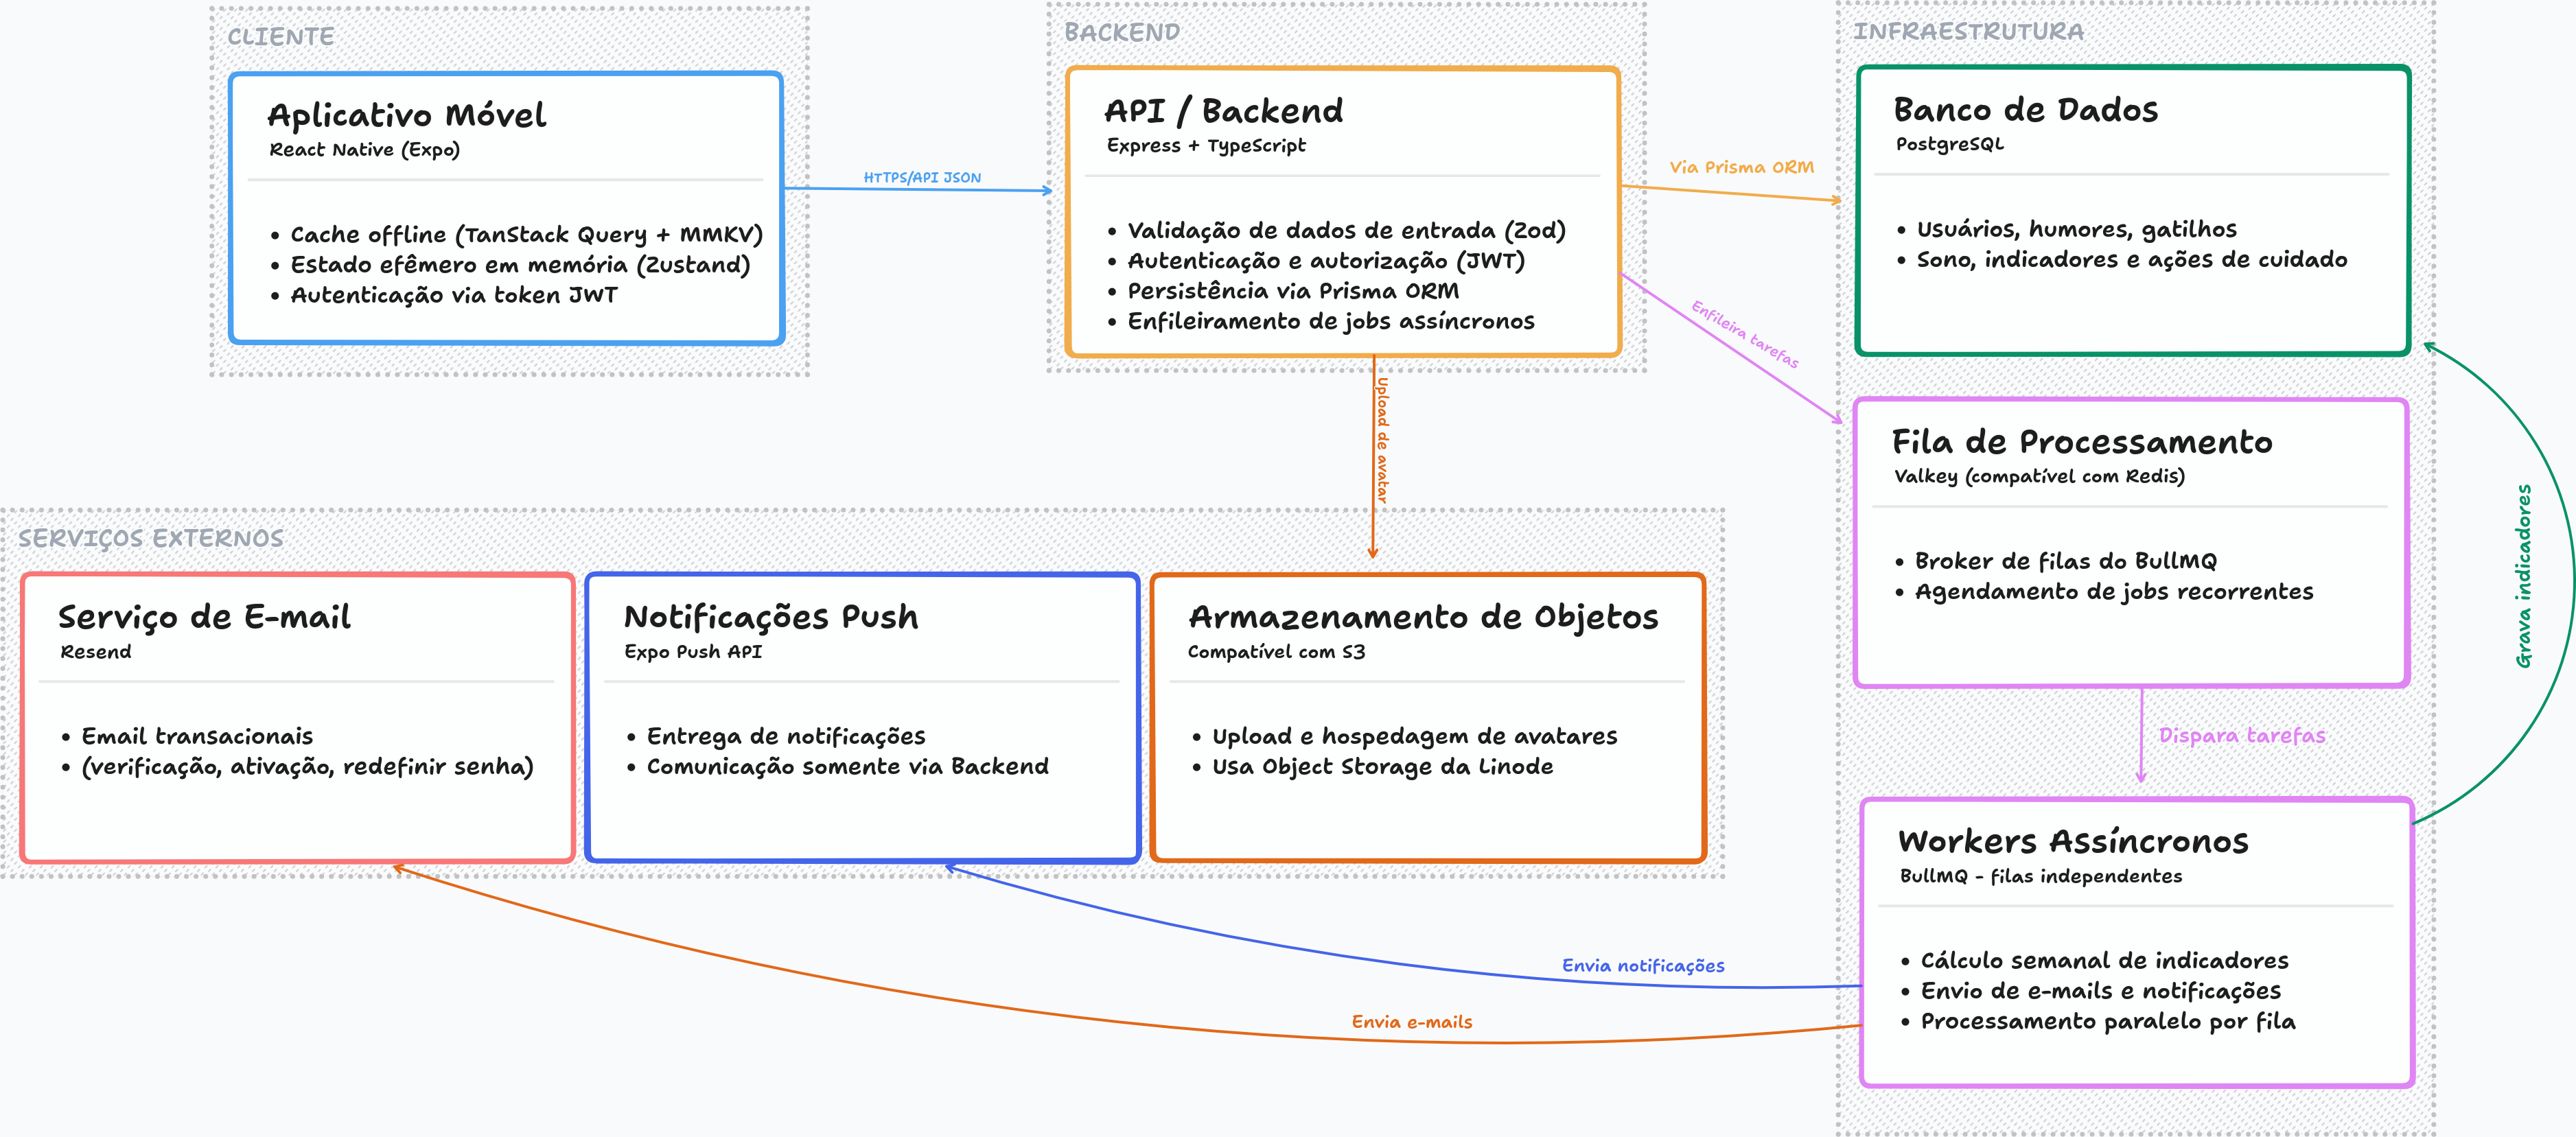
\includegraphics[width=0.9\linewidth]{arch-v2.png}
\source{Elaborado pelo autor (2026)}
\end{figure}


Este capítulo detalha o funcionamento de algumas funcionalidades
desenvolvidas durante o projeto. Apenas algumas funcionalidades mais
chaves são abordadas neste capítulo, como o registro de humor, vinculo
de um gatilho, indicadores, e o registro de atividades.

\section{Processo de Login}

Logo ao abrir o aplicativo, o usuário é redirecionado para a tela de
login. A tela em si é relativamente simples, e contém os campos de
email e senha. Existe aqui um elemento proposital: uma forma de
garantir um certo nível de anonimato, em que o usuário não precisa se
identificar com um nome ou número de telefone, tampouco ativar a conta
através de uma plataforma de terceiro, como Google ou Facebook.

Isso se dá, em especial, por dois motivos. Primeiro, o uso de uma tecnologia de
autenticação, como por exemplo, \textit{OAuth} \cite{Hardt:2012} exigiria uma
conexão com plataformas de terceiro, que poderiam então rastrear quais usuários
têm acesso a qual aplicativo --- algo que é fartamente documentado na literatura
sobre os mecanismos usados por tais plataformas para rastrear e monitorar o
acesso a dados de usuários, com o fim de vender e monetizar essas informações.

Essa preocupação não é hipotética: um estudo que interceptou o tráfego de rede
de 36 dos aplicativos mais populares de saúde mental (depressão e cessação de
tabagismo) encontrou transmissão de dados a pelo menos um terceiro em 92\%
deles, sendo que 81\% enviavam dados especificamente a serviços operados por
Google ou Facebook --- e apenas 59\% desses casos declaravam esse
compartilhamento em política de privacidade \cite{Huckvale2019}.

Um estudo posterior, focado exclusivamente em 27 aplicativos de saúde
mental mais populares da Google Play Store, confirmou o mesmo padrão e
o caracterizou formalmente como uma ameaça:

\begin{quote}
  A maioria dos aplicativos representa ameaças relacionadas à rastreabilidade,
  à identificação e à detecção. Isso constitui um risco, pois  alguns terceiros
  podem rastrear, reidentificar e detectar as ações e os dados dos usuários. A
  falta de conscientização também está relacionada a essas ameaças, uma vez que
  os aplicativos não explicam (por exemplo, na política de privacidade) os
  riscos que a publicidade direcionada representa para pessoas com problemas
  mentais, bem como o risco de reidentificação e divulgação de condições de
  saúde mental (por exemplo, ansiedade, depressão).
  \cite[p.~3, tradução nossa]{Iwaya:22}
\end{quote}

Como os próprios autores resumem, a mera vinculação de um usuário a um
aplicativo de saúde mental já pode revelar que essa pessoa possui uma condição
psicológica --- seja ansiedade, depressão, ou, no caso de um aplicativo como o
Nexo, Transtorno Afetivo Bipolar ---, tornando usuários desses aplicativos
particularmente vulneráveis a esse tipo de exposição \cite{Iwaya:22}.

No caso do Nexo, essa cadeia de inferência é especialmente
sensível: a presença do aplicativo na lista de apps instalados de um usuário,
associada ao seu identificador publicitário, permitiria a uma plataforma como a
Meta inferir uma possível condição de saúde mental do usuário para fins de
segmentação de anúncios, sem que este tenha conhecimento ou consentimento
explícito disso.

Segundo, e retomando a proposta de oferecer ao usuário a possibilidade
de \textit{self-service}, aquele que decidisse manter uma instância
própria do aplicativo não precisaria de uma conta em uma plataforma de
terceiro, nem se cadastrar nelas.

\begin{figure}[H]
\centering
\caption{Tela de login}
\label{fig:screenshot-login}
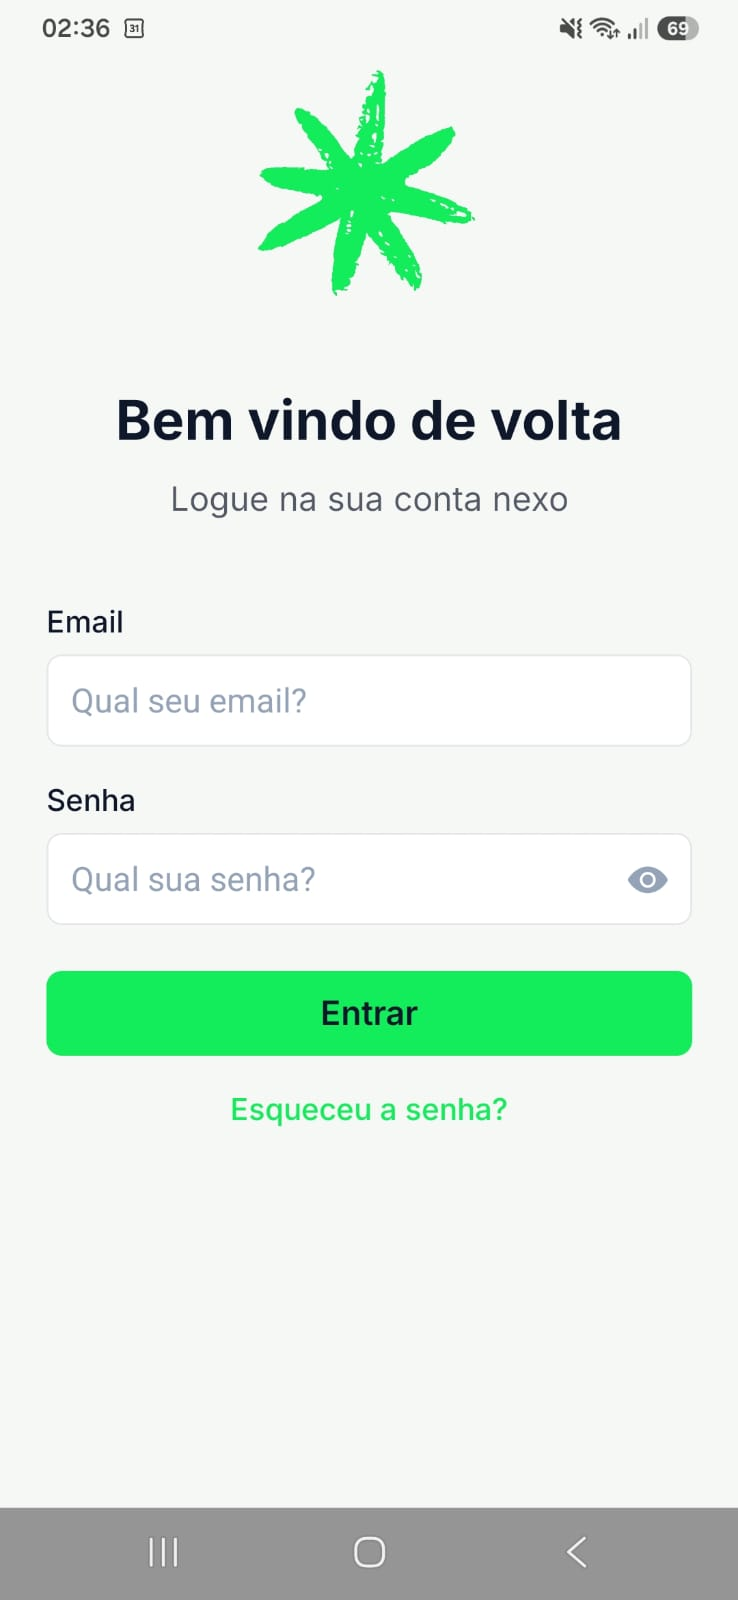
\includegraphics[width=0.70\textwidth,height=0.60\textheight,keepaspectratio]{screenshot-login.jpeg}
\source{Elaborado pelo autor (2026)}
\end{figure}

Por fim, destaca-se aqui que, conforme mencionado anteriormente na
modelagem de casos de uso (figura \ref{fig:use-cases}), ao realizar o
login pela primeira vez é enviado um email com um código de
verificação, seguindo a lógica dos \textit{magic links}. Isso adiciona
uma camada extra de segurança, garantindo que apenas o usuário que
solicitou o login possa acessar a conta.

\section{Página de Consulta de Registros}

A tela inicial é a tela nomeada apenas como ``Novo''. A proposta aqui
é ser a tela de cadastro rápido de um humor, e também é a tela que
visualmente mais destoa das demais. O usuário é apresentado com três
seções distintas:

\begin{itemize}
    \item Cadastro rápido de um humor
    \item Entre ontem e hoje
    \item Registros recentes
\end{itemize}

Respectivamente: uma seção em que o usuário é convidado a ``escolher
um humor'' e iniciar o processo de registro de uma nova entrada; a
seção em que são apresentados os indicadores de nível de energia
acumulado entre o dia anterior e o dia atual, além da média de sono do
dia comparada com a do dia anterior; e, por fim, a listagem dos dez
últimos registros de humor cadastrados pelo usuário.

\begin{figure}[H]
\centering
\caption{Tela de Consulta de Registros}
\label{fig:screenshot-consulta-registros}
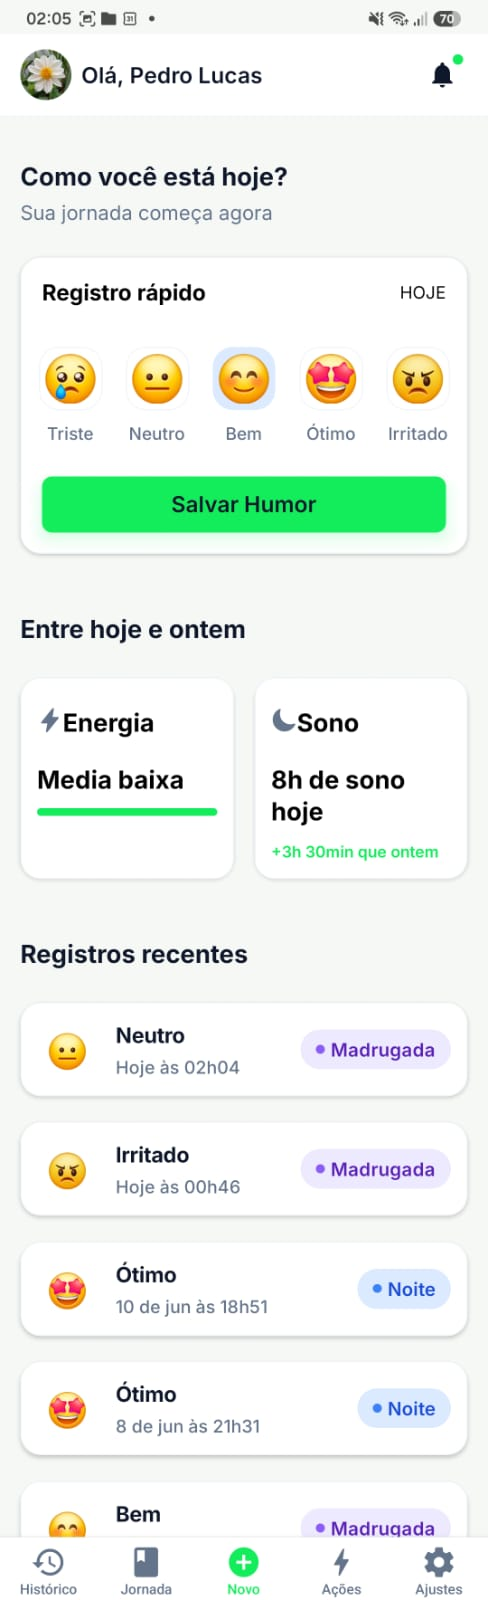
\includegraphics[width=0.70\textwidth,height=0.60\textheight,keepaspectratio]{screenshot-initial-page.jpeg}
\source{Elaborado pelo autor (2026)}
\end{figure}

Aqui já é introduzido ao usuário um padrão de organização e hierarquia:
todos os elementos centrais são organizados em \textit{cards}, exibidos
em no máximo duas colunas. Também é introduzido, caso o usuário já
possua registros de humor cadastrados, o padrão pelo qual esses
registros são resumidos em todas as seções do aplicativo: geralmente
um ícone, um título e alguma informação adicional em destaque.

\section{Criação de Registros de Humor}

Nesta seção, o usuário pode criar novos registros de humor, escolhendo
entre uma lista de opções pré-definidas. O humor selecionado na tela
anterior é mostrado aqui, e o usuário é convidado a julgar, em uma
escala de 1 a 10, como se sente em relação aos níveis de energia,
estresse e ansiedade, respectivamente.

\begin{figure}[H]
\centering
\caption{Criação de Registros de Humor}
\label{fig:screenshot-consulta-humor}
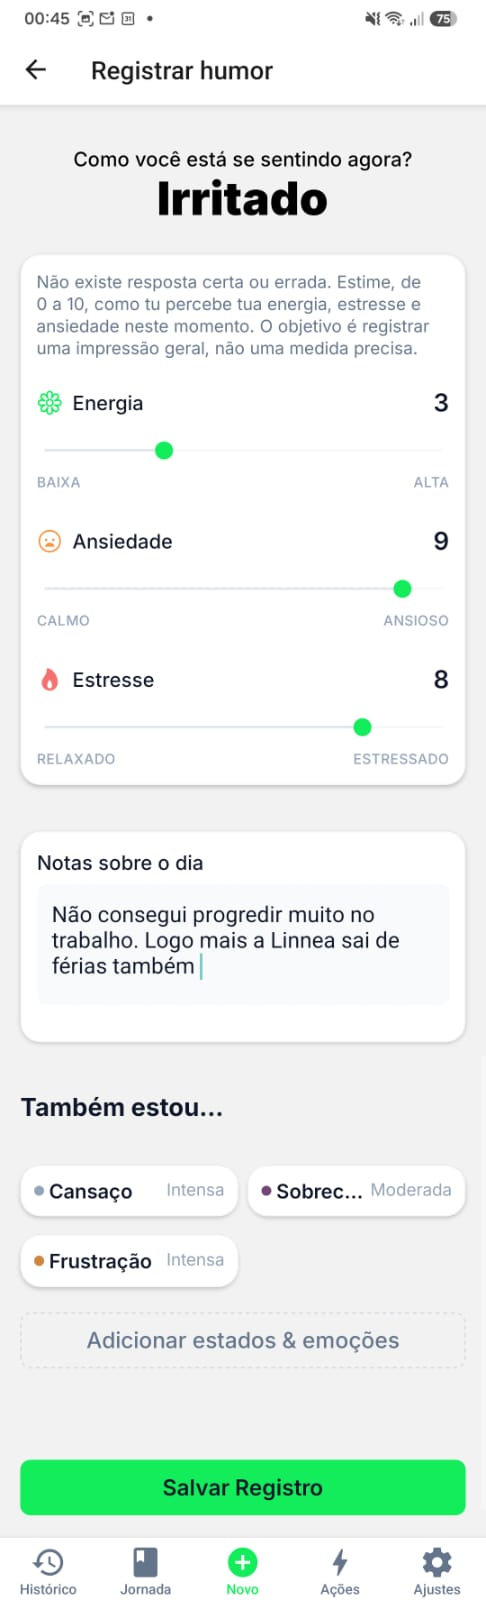
\includegraphics[width=0.70\textwidth,height=0.60\textheight,keepaspectratio]{screenshot-create-mood.jpeg}
\source{Elaborado pelo autor (2026)}
\end{figure}

Naturalmente, é uma questão difícil de responder --- e, como o próprio
aplicativo procura deixar claro, é importante que seja um momento
reflexivo, não necessariamente preciso.

O usuário pode adicionar uma anotação sobre aquele registro em
específico, padrão que se repete em outras telas do aplicativo.

Por fim, o usuário pode escolher o que compõe aquele registro, ou
seja, selecionar emoções e estados/sentimentos que sente naquele
momento. É apresentada uma listagem mista desses elementos, na qual o
usuário seleciona os que mais se aplicam a ele e atribui um nível de
intensidade para cada um. Aqui a escala é menor e mais simples, visando
facilitar a escolha e o julgamento do usuário, entre ``Leve'',
``Moderado'' e ``Intenso'', conforme a figura
\ref{fig:screenshot-add-components}.

\begin{figure}[H]
\centering
\caption{Adicionando sentimentos/emoções}
\label{fig:screenshot-add-components}
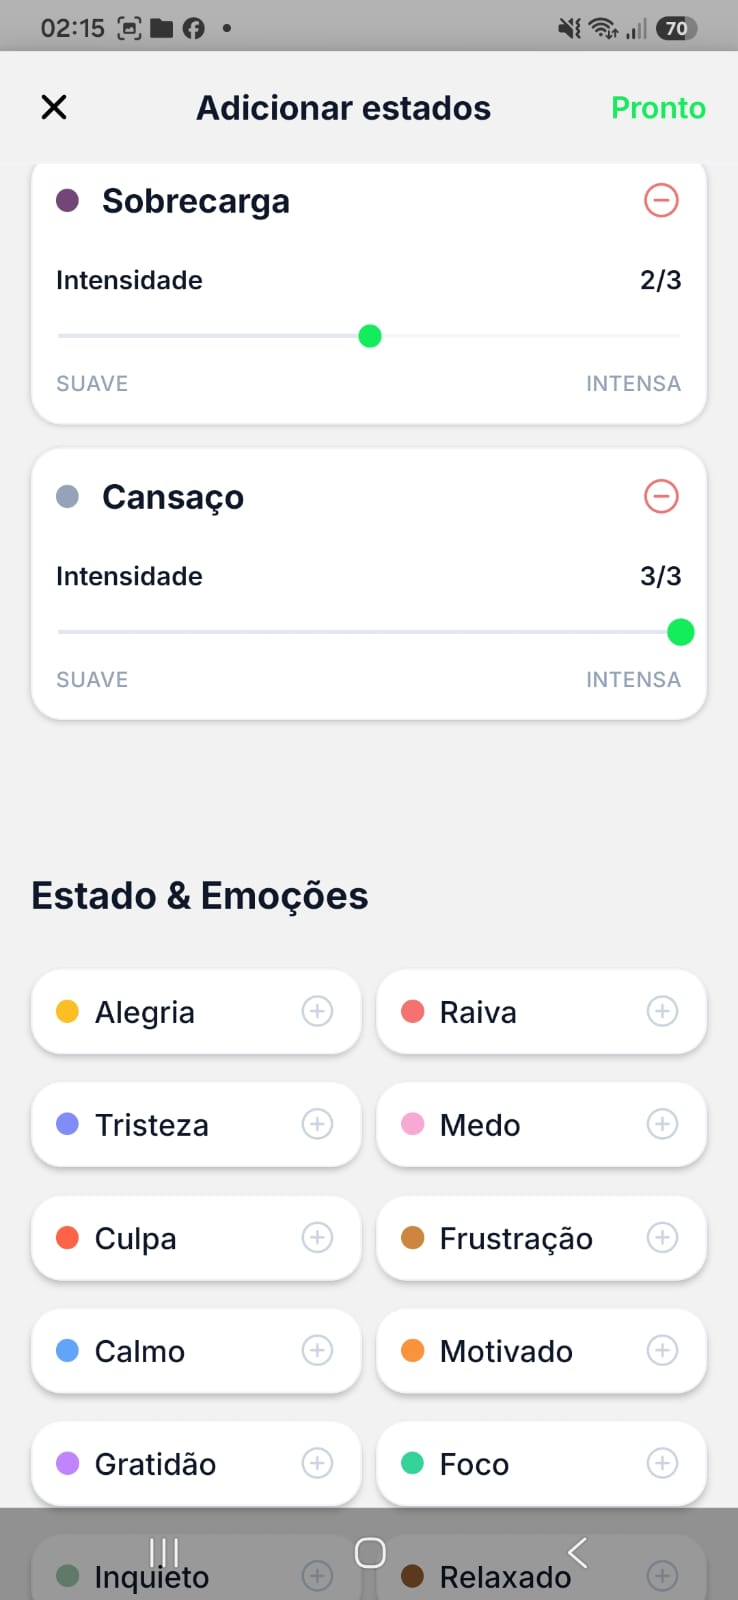
\includegraphics[width=0.70\textwidth,height=0.60\textheight,keepaspectratio]{screenshot-add-components.jpeg}
\source{Elaborado pelo autor (2026)}
\end{figure}

Ao concluir esse processo e salvar, é apresentada ao usuário uma tela
de confirmação, na qual ele pode, opcionalmente, vincular o registro a
um gatilho específico --- que pode ter ocorrido antes de ele salvar o
registro --- ou criar um novo gatilho. O projeto novamente se ancora no
EMA, enriquecendo o registro de humor com mais contexto sobre o que
aconteceu.

\begin{figure}[H]
\centering
\caption{Vinculando um humor com um gatilho}
\label{fig:screenshot-link-mood-trigger}
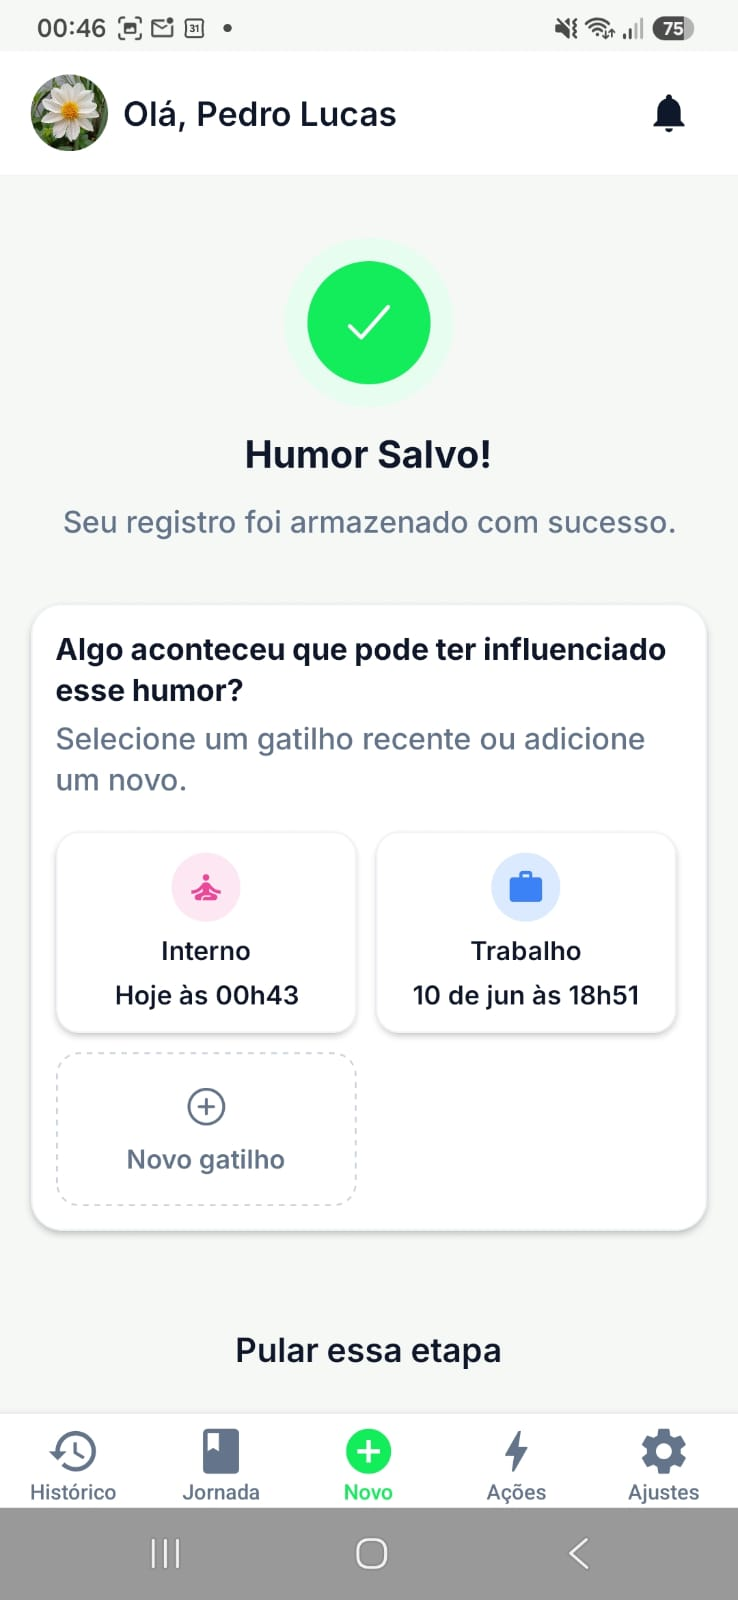
\includegraphics[width=0.70\textwidth,height=0.60\textheight,keepaspectratio]{screenshot-link-mood-with-trigger.jpeg}
\source{Elaborado pelo autor (2026)}
\end{figure}

Em seguida, o usuário pode indicar o impacto que aquele gatilho
exerceu sobre o registro de humor em questão. Novamente, trata-se de
uma estimativa subjetiva, sem pretensão de precisão.

\begin{figure}[H]
\centering
\caption{Avaliando o impacto de um gatilho no humor}
\label{fig:screenshot-assess-trigger-mood-impact}
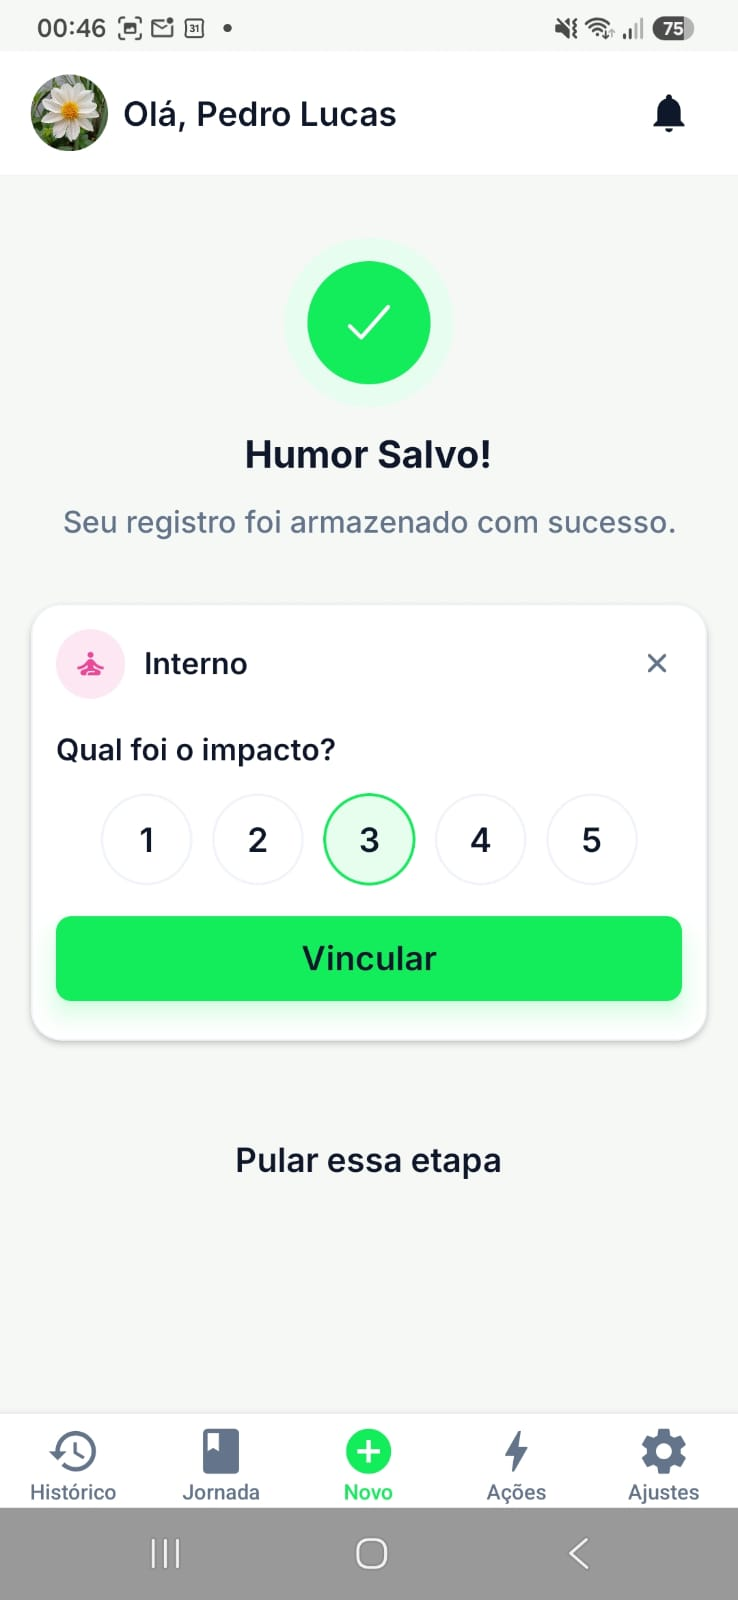
\includegraphics[width=0.70\textwidth,height=0.60\textheight,keepaspectratio]{screenshot-link-mood-assess-impact.jpeg}
\source{Elaborado pelo autor (2026)}
\end{figure}

Por fim, vale mencionar que, após esse processo, é enfileirado
internamente um \textit{background job} que recalcula, sob demanda, o
indicador de energia daquele dia, apresentado na figura
\ref{fig:screenshot-consulta-registros}. Diferentemente deste, os
indicadores semanais --- como a correlação entre sono e energia,
descrita na seção \ref{sec:insights} --- não são recalculados a cada
registro individual, sendo processados apenas pelo job semanal
agendado (seção \ref{sec:insights}).

\section{Indicadores}\label{sec:insights}

Nessa tela é apresentado um conjunto de indicadores construídos a partir
dos registros de humor, sono e gatilho do usuário. Diferente das demais
telas do aplicativo, que operam sobre dados em tempo real, os indicadores
são artefatos pré-computados: um \textit{worker} assíncrono (\textit{BullMQ})
percorre semanalmente todos os usuários ativos e enfileira, para cada
um, um conjunto de \textit{jobs} --- um por tipo de indicador --- que
processam a janela dos últimos sete dias e persistem o resultado em uma
tabela dedicada. Vale notar que nem todos os indicadores seguem esse
fluxo agendado: os indicadores diários (energia e sono) são recalculados
sob demanda, no momento em que o usuário registra um novo humor ou
sessão de sono, enquanto os indicadores semanais dependem
exclusivamente do \textit{job} de \textit{fan-out} de segunda-feira.

O aplicativo móvel apenas consulta esse resultado já
calculado, o que evita repetir cálculos custosos a cada abertura da tela
e desacopla a lógica analítica do restante da API.

\begin{figure}[H]
\centering
\caption{Tela de indicadores}
\label{fig:screenshot-insights}
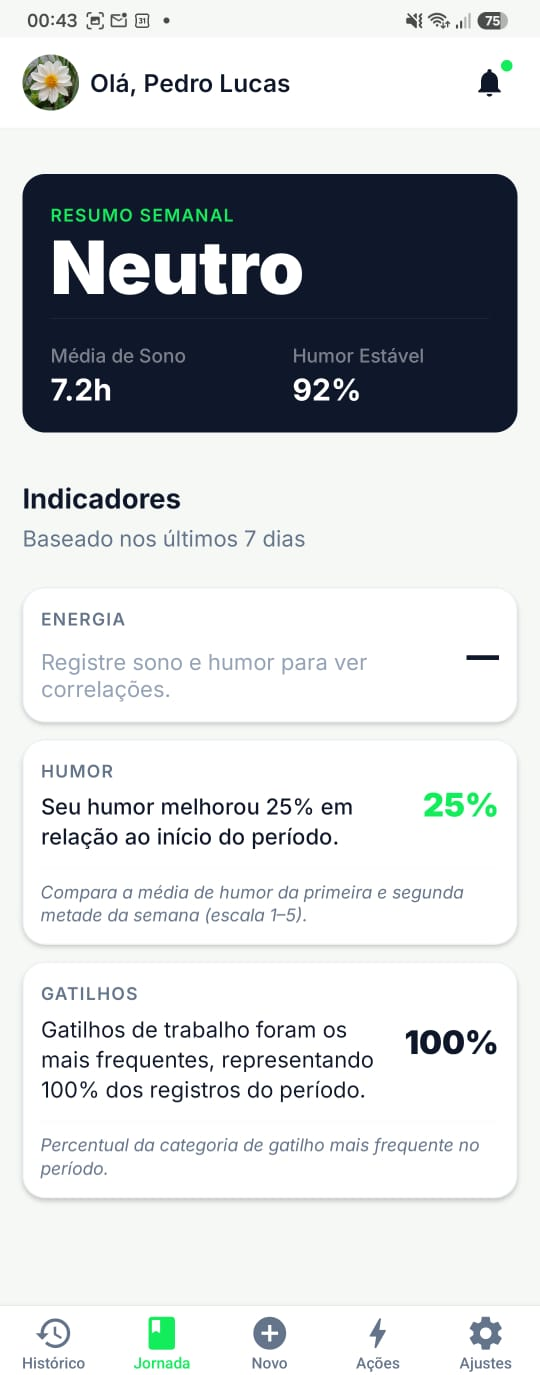
\includegraphics[width=0.70\textwidth,height=0.60\textheight,keepaspectratio]{screenshot-insights.jpeg}
\source{Elaborado pelo autor (2026)}
\end{figure}

% TODO: referenciar EMA / momentary assessment como justificativa da janela de 7 dias

São três os indicadores semanais exibidos: tendência de humor, correlação
entre sono e energia, e padrão de gatilhos.

\begin{itemize}
    \item \textbf{Tendência de humor}: compara a média de humor da
    primeira metade da semana com a da segunda metade, expressando a
    diferença como uma variação percentual. O resultado é classificado
    como melhora, piora ou estabilidade a partir de uma margem de $\pm10\%$.

    \item \textbf{Correlação entre sono e energia}: relaciona a duração
    do sono de uma noite com o nível de energia relatado na manhã
    seguinte, através do coeficiente de correlação de Pearson. Exige um
    mínimo de observações pareadas para ser calculado --- caso contrário,
    o indicador simplesmente não é exibido.

    \item \textbf{Padrão de gatilhos}: identifica a categoria de gatilho
    mais frequente na semana e expressa sua predominância como percentual
    do total de registros.
\end{itemize}

É intencional, na figura \ref{fig:screenshot-insights}, que o bloco de
``Energia'' apareça vazio: o cálculo da correlação depende da existência
simultânea de registros de sono \emph{e} de humor em quantidade mínima,
e no período retratado o usuário ainda não havia acumulado dados
suficientes de ambos os tipos. Optou-se por não exibir uma correlação
calculada com poucos pontos, preferindo comunicar a ausência de dado a
apresentar um número pouco confiável.

O bloco maior no topo da tela, o ``Resumo Semanal'', condensa os
indicadores mais centrais --- média de sono do período e um rótulo de
humor (``Estável'', no exemplo). Esse rótulo, no entanto, é o elemento
mais delicado de toda a funcionalidade. Embora exista uma fórmula capaz
de produzir uma classificação de estabilidade a partir da variância dos
registros de humor, atribuir esse tipo de afirmação a um usuário ---
especialmente em um aplicativo que é utilizado por pessoas com
Transtorno Afetivo Bipolar, para quem uma leitura equivocada de
``estabilidade'' pode mascarar justamente o início de um episódio ---
exige um embasamento mais cuidadoso do que uma regra estatística
simples. Por esse motivo, o rótulo apresentado nesta versão do
aplicativo é estático (não deriva de fato do cálculo de estabilidade) e
a funcionalidade pode ser inteiramente desabilitada pelo usuário nas
configurações. A decisão de manter ou não uma afirmação automatizada
desse tipo, e sob quais critérios, permanece um ponto em aberto que
mereceria revisão de literatura específica antes de ser tratado como
funcionalidade definitiva.

% TODO: literatura sobre riscos de auto-monitoramento automatizado de humor / mood-tracking apps e TAB

\section{Histórico}\label{sec:history-analysis}

Nessa tela é apresentado o histórico consolidado de registros de humor,
sono, gatilho e ações de cuidado (como sessões de terapia), organizados
cronologicamente e agrupados por dia, conforme a figura
\ref{fig:screenshot-history}. O usuário pode ainda filtrar a listagem por
categoria (``Humor'', ``Sono'', ``Gatilho'' e ``Ações de Cuidado''),
reduzindo o volume de informação exibida.

\begin{figure}[H]
\centering
\caption{Tela de Histórico}
\label{fig:screenshot-history}
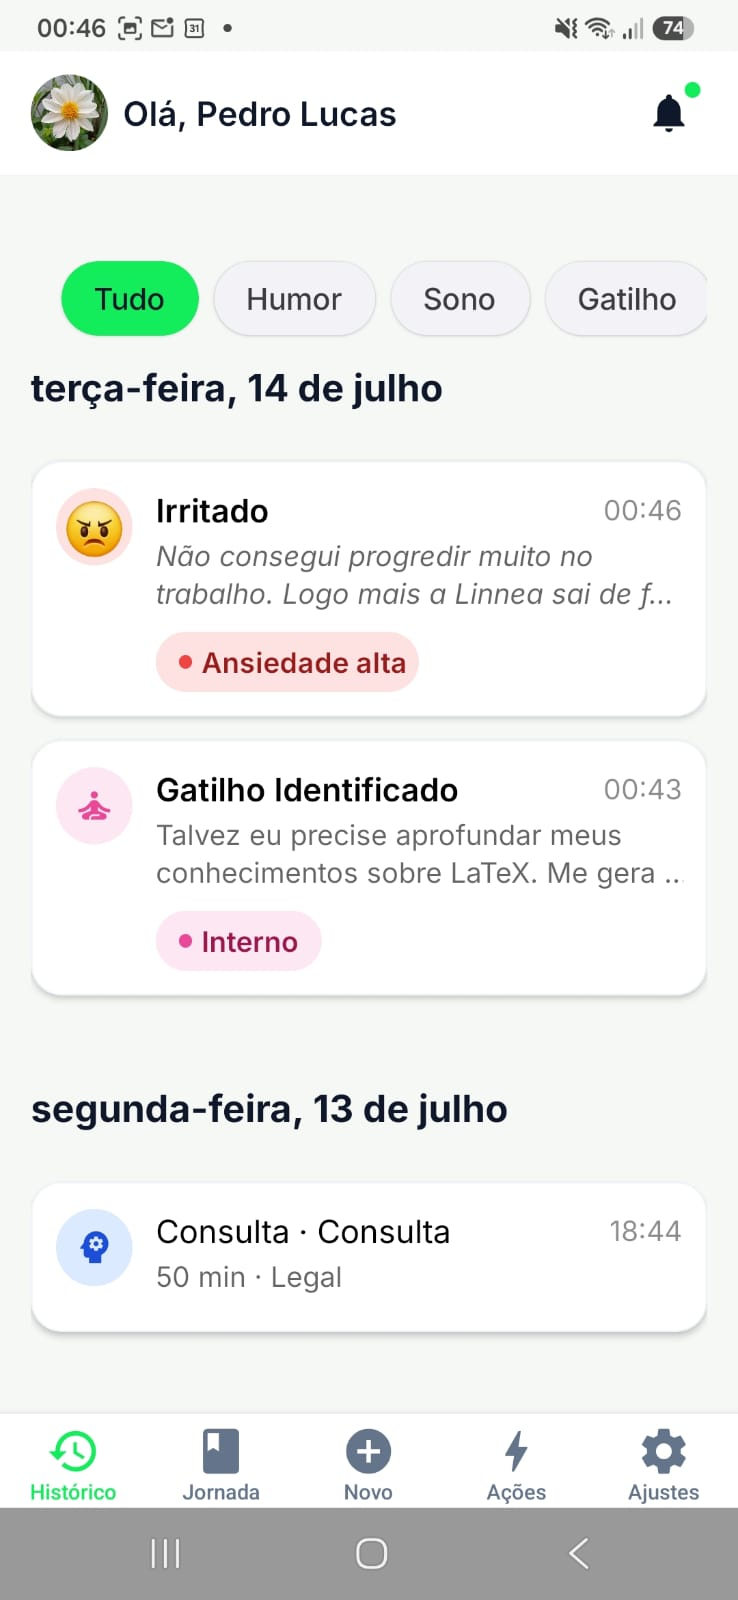
\includegraphics[width=0.70\textwidth,height=0.60\textheight,keepaspectratio]{screenshot-history.jpeg}
\source{Elaborado pelo autor (2026)}
\end{figure}

Como os quatro tipos de dado residem em recursos distintos da API, a
tela consulta os respectivos \textit{endpoints} em paralelo e, em
seguida, processa o resultado no próprio aplicativo. Para isso, é
utilizado um pequeno serviço que atua como \textit{mapper}, transformando
os dados de cada \textit{endpoint} em um formato comum, apresentado no
código \ref{lst:history-card}.

\newpage

\begin{lstlisting}[caption={Formato comum da tela de histórico}, label={lst:history-card}]
export type HistoryCard = {
  id: string; // "<category>-<id>" to avoid collisions
  category: HistoryCategory;
  subtype?: CareActionSubtype; // only set when category === "care_action"
  timestamp: string; // ISO string -- used for sorting and display
  title: string;
  summary: string;
  badge?: HistoryBadge;
  raw: MoodEntry | SleepRecord | Trigger | CareAction;
};
\end{lstlisting}

Após a normalização, os quatro conjuntos de dados são combinados em uma
única lista ordenada pelo campo \texttt{timestamp} e reagrupados por dia
para exibição, conforme visto na figura \ref{fig:screenshot-history}, nos
cabeçalhos ``terça-feira, 14 de julho'' e ``segunda-feira, 13 de julho''.
Essa unificação é proposital: ao invés de apresentar quatro telas
separadas por tipo de dado, o histórico busca reconstruir uma narrativa
única do dia do usuário, aproximando-se do princípio de \textit{Ecological
Momentary Assessment} já mencionado anteriormente --- o contexto de um
registro de humor (por exemplo, o gatilho ``Interno'' registrado três
minutos antes, na mesma figura) fica visualmente próximo do evento que
possivelmente o motivou.

A propriedade \texttt{raw} armazena o dado original, permitindo que a
listagem redirecione o usuário para a tela de detalhe correta ao tocar em
um card, independentemente da categoria. Já a propriedade \texttt{badge}
reaproveita o mesmo mecanismo já descrito na seção de indicadores: para
um registro de sono, sinaliza se a duração foi insuficiente; para um
registro de humor, destaca a dimensão mais relevante daquele registro
(como ``Ansiedade alta'' na figura \ref{fig:screenshot-history}); para um
gatilho, indica sua categoria, e assim por diante.

\FloatBarrier

\chapter{Testes}\label{cap:testes}

Este capítulo registra como o comportamento do Nexo é verificado. Como nos
capítulos anteriores, o compromisso é com a honestidade: não se prescreve uma
estratégia ideal, mas se descreve o estado da prática, o que cada tipo de teste
é capaz --- e incapaz --- de detectar, e as lacunas assumidas explicitamente na
Seção~\ref{sec:test-gaps}.

O foco recai sobre a verificação automatizada. A validação com usuários reais
não foi realizada neste trabalho: o envolvimento de participantes em uma
aplicação de saúde mental exigiria aprovação prévia de comitê de ética em
pesquisa, levantamento de pessoas com transtorno de forma a aplicar com elas,
cujo todo o trâmite não coube no cronograma do projeto. Essa ausência de
avaliação externa é retomada como limitação na Seção~\ref{sec:test-gaps}.

Os dados quantitativos citados ao longo do capítulo referem-se ao estado do
repositório em meados de outubro de 2026.

\section{Vocabulário}\label{sec:test-vocab}

Quatro termos delimitam o alcance dos testes descritos adiante: unitário,
integração, \textit{job} e \textit{end-to-end} (E2E). Como os nomes e as
fronteiras entre esses níveis variam entre autores, o Quadro~\ref{tab:test-vocab}
fixa o sentido adotado neste trabalho e o relaciona aos níveis usuais da
literatura.

\begin{table}[H]
\centering
\caption{Vocabulário de testes adotado neste trabalho}
\label{tab:test-vocab}
\small
\begin{tabular}{|p{2.8cm}|p{6.6cm}|p{4.2cm}|}
\hline
\textbf{Termo} &
\textbf{O que exercita} &
\textbf{Nível usual na literatura} \\

\hline

Teste unitário &
Uma única função ou módulo, sem HTTP e sem banco de dados. &
Teste de unidade. \\

\hline

Teste de integração &
A aplicação HTTP real (rotas, validação, autenticação, controladores
e serviços) sobre um banco de dados real; apenas o que sai do processo
é simulado &
Teste de integração, em nível de API. \\

\hline

Teste de \textit{job} &
Um processador de tarefa em segundo plano, chamado diretamente com uma carga
fabricada, sobre o banco real. &
Teste de integração de componente assíncrono \\

\hline

Teste \textit{end-to-end} (E2E) &
O aplicativo empacotado, em um dispositivo, ao longo de uma jornada real de
usuário. &
Teste de sistema. \\

\hline
\end{tabular}
\source{Elaborado pelo autor (2026)}
\end{table}

\section{Estratégia de Verificação}\label{sec:test-strategy}

O código-fonte do Nexo vive em um único repositório com dois projetos
independentes: a API e o aplicativo móvel. O esforço de teste entre eles é
deliberadamente assimétrico. A API possui uma suíte automatizada e é protegida
por um portão de integração contínua; o aplicativo móvel é verificado
majoritariamente de forma manual, com uma suíte \textit{end-to-end} fina por
cima. Essa assimetria não é um descuido, e se justifica por duas prioridades.
A primeira é a capacidade de trabalho limitada: manter uma suíte automatizada
completa nas duas esferas excederia o disponível, e concentra-se o esforço onde
o retorno é maior. A segunda é que a API concentra a validação, a autenticação,
as regras de negócio e a persistência --- isto é, a garantia sobre a integridade
dos dados registrados pelo usuário.

A Tabela~\ref{tab:test-tooling} resume as ferramentas envolvidas e o ponto em que
cada uma atua.

\begin{table}[H]
\centering
\caption{Ferramentas de verificação}
\label{tab:test-tooling}
\small
\begin{tabular}{|p{4.4cm}|p{4.0cm}|p{5.0cm}|}
\hline
\textbf{Finalidade} &
\textbf{Ferramenta} &
\textbf{Onde atua} \\

\hline

Execução de testes e asserções da API &
Vitest &
API \\

\hline

Requisições HTTP nos testes &
Supertest &
Dentro dos arquivos do Vitest \\

\hline

Cobertura de código da API &
Vitest (\textit{coverage}) &
API, sem limiar mínimo \\

\hline

Banco de dados de teste &
PostgreSQL &
\textit{Container} local durante desenvolvimento; serviço efêmero no CI \\

\hline

Testes \textit{end-to-end} móveis &
Maestro &
Dispositivo Android físico, via \textit{adb} \\

\hline

\textit{Lint} do aplicativo &
ESLint (\texttt{expo lint}) &
Manual, fora do CI \\

\hline

Integração contínua &
GitHub Actions &
API \\

\hline
\end{tabular}
\source{Elaborado pelo autor (2026)}
\end{table}

\section{Suíte de Testes da API}\label{sec:test-api}

A suíte automatizada concentra-se na API e cobre três frentes: os testes
unitários, os testes de integração das rotas HTTP e os testes dos processadores
de tarefas em segundo plano. No momento da redação, o diretório
\texttt{api/tests} reunia 48 arquivos --- 17 unitários, 26 de rotas e cinco de
\textit{jobs}. A execução e as asserções ficam a cargo do Vitest; as requisições
HTTP são feitas pelo Supertest, que exercita a aplicação Express diretamente,
sem abrir uma porta de rede, porém através de sua pilha HTTP real.

\subsection{Organização e ferramentas}\label{sec:test-api-org}

A configuração do Vitest (\texttt{api/vitest.config.ts}) divide a suíte em dois
``projetos''. O projeto \texttt{unit} seleciona os arquivos com o sufixo
\texttt{.unit.test.ts} e não carrega configuração global alguma, de modo que
esses testes dependem apenas das funções que exercitam. O projeto \texttt{db}
seleciona os demais arquivos --- integração e \textit{job} ---, aplica um arquivo
de configuração global, fixa um limite de tempo por teste e faz com que esses
testes trunquem e repovoem o banco.

A cobertura de código é apenas mensurada, não imposta: o relatório
(\texttt{npm run test:coverage}) não possui limiar mínimo nem bloqueia a
integração contínua. A verificação estática de tipos (\texttt{npm run typecheck})
também roda em caráter consultivo no CI --- uma falha é registrada, mas não
interrompe o \textit{deploy}.

\subsection{Execução e banco de dados de teste}\label{sec:test-api-db}

Os testes que dependem do banco rodam contra uma instância real do PostgreSQL
--- e não contra um substituto em memória ---, em uma base dedicada de nome
sufixado com \texttt{\_test}, criada por um pequeno script e materializada com
\texttt{prisma db push}. O isolamento entre os casos é obtido por truncamento:
antes de cada teste, uma rotina executa \texttt{TRUNCATE users CASCADE},
removendo a tabela de usuários e, por cascata, todas as dependentes. Não há
\textit{rollback} transacional nem banco efêmero por execução.

O carregamento de dados é feito por funções auxiliares escritas à mão, e não por
uma biblioteca de fábricas: um módulo compartilhado
(\texttt{api/tests/test-helper.ts}) oferece as primitivas centrais --- cliente
Prisma, limpeza da base, criação de usuário e geração de token ---, e cada
arquivo define os \textit{seeders} de que necessita.

A regra para o uso de dublês na API é: simula-se apenas o que deixa o processo;
a aplicação e o banco permanecem reais. A camada de filas (BullMQ) é substituída
globalmente por um substituto que registra os \textit{jobs} enfileirados,
permitindo afirmar tanto a resposta HTTP quanto o trabalho em segundo plano
agendado. O envio de arquivos e o cliente de armazenamento são substituídos por
implementações controladas, e o disparo de e-mail e de notificações
\textit{push} é simulado pontualmente, nos arquivos que os exercitam.

Duas fronteiras permanecem deliberadamente reais: o acesso ao banco, via
Prisma, nunca é simulado; tampouco a autenticação. Os testes geram tokens JWT
válidos, assinados com o segredo de teste, e os enviam no cabeçalho de
autorização, de modo que o \textit{middleware} de autenticação real seja
executado. Essa escolha reduz o risco de um teste passar porém se comportar de
maneira distinta em produção.

\subsection{Tipos de testes}\label{sec:test-api-tipos}

A suíte da API divide-se em três grupos, retomando o vocabulário do
Quadro~\ref{tab:test-vocab}: unitários, integração e tarefas assíncronas. Cada
grupo é descrito a seguir com o que exercita, o que detecta e o que escapa ao
seu alcance.

\subsubsection{Testes unitários}

Os testes unitários exercitam uma única função ou módulo, sem HTTP e sem banco
de dados. Concentram-se na lógica pura do sistema, em grande parte extraída
deliberadamente de seus envoltórios de persistência para se tornar testável: os
agregadores dos indicadores, os construtores dos relatórios e auxiliares
compartilhados, como paginação e conversão de agendamento. Também cobrem o
gerador de código de ativação, a validade de tokens, os serializadores e as
regras de validação. Por serem rápidos e determinísticos, são o instrumento
natural para fixar casos-limite --- fronteiras de janelas de tempo, margens de
classificação e aritmética de paginação --- e servem como documentação
executável dessas regras.

A limitação desse nível é estrutural: ele só alcança a lógica isolada em uma
costura testável. Sem o banco e a camada HTTP, a maior parte do comportamento
permanece fora de alcance, e o nível pouco contribui, isoladamente, para a
confiança geral na aplicação.

\subsubsection{Testes de integração}

Os testes de integração formam a maior parte da suíte. Cada um constrói a
aplicação real, conecta um cliente Prisma real e a exercita via Supertest,
afirmando tanto a resposta HTTP quanto o estado persistido. Eles percorrem o
caminho completo de uma requisição --- roteamento, validação, autenticação,
controladores, serviços e persistência --- e, por operarem sobre um PostgreSQL
real, não sofrem o descolamento que afeta os substitutos. Afirmar a resposta e
as linhas persistidas simultaneamente verifica o efeito da operação, e não
apenas o valor de retorno.

Em contrapartida, exigem infraestrutura em execução, são mais lentos e, por
compartilharem a mesma base, rodam em série. O isolamento por truncamento é
suficiente, porém menos rigoroso do que um \textit{rollback} transacional, pois
um teste que falha no meio pode deixar resíduos.

\subsubsection{Testes de tarefas assíncronas}

Os testes de \textit{jobs} importam um processador do BullMQ e o chamam
diretamente, com uma carga fabricada, contra o banco real. Cobrem o código que
executa fora do ciclo requisição--resposta --- os \textit{workers} que geram
exportações, enviam mensagens e recalculam indicadores ---, chegando, no caso
da exportação, a descompactar o anexo produzido e inspecionar seu conteúdo.

Como o processador é invocado diretamente, a maquinaria da fila em si ---
agendamento, repetição, tentativas e ordenação --- permanece fora do alcance. A
carga é fabricada à mão e, por isso, pode divergir daquela que o enfileirador
realmente envia, sem que nada verifique uma contra a outra.

\section{Verificação do Aplicativo Móvel}\label{sec:test-mobile}

Em linha com a assimetria descrita na Seção~\ref{sec:test-strategy}, o
aplicativo móvel passou a contar com testes unitários em estágio inicial, ainda
em andamento e sem a cobertura da suíte da API. A verificação cotidiana
permanece predominantemente manual, em um dispositivo físico, contra a pilha
local em execução --- o aplicativo roda como \textit{build} de desenvolvimento
do Expo, com dependências nativas do Android. Essa verificação captura o que os
testes automatizados raramente alcançam --- problemas visuais, de leiaute e de
desempenho no dispositivo ---, mas não é repetível, não protege contra
regressões e permanece invisível à integração contínua.

\subsection{Suíte \textit{end-to-end} (Maestro)}\label{sec:test-mobile-e2e}

Sobre a verificação manual há uma suíte \textit{end-to-end} opcional, baseada
no Maestro, ferramenta declarativa de automação de interface para dispositivos
móveis. A suíte cobre uma única jornada central --- login, registro de humor e
saída --- por três fluxos em YAML, marcados como \texttt{smoke} e executados
por um pequeno \textit{harness} (\texttt{frontend/scripts/e2e.sh}), exposto
como \texttt{npm run test:e2e}. Os fluxos são dirigidos por identificadores de
teste (\texttt{testID}) inseridos no código, e não pelo texto visível, o que os
torna mais robustos a mudanças de interface.

A execução depende de um dispositivo Android físico conectado por \texttt{adb},
de um \textit{build} de desenvolvimento, da API em funcionamento com um usuário
de teste semeado e do Metro servindo o aplicativo; não há caminho sem cabeça
nem integração ao CI, de modo que a suíte é executada manualmente e com pouca
frequência. Cada fluxo limpa o estado do aplicativo e recarrega o
\textit{bundle}, tornando a execução lenta, e a cobertura permanece fina: um
único caminho feliz, sem casos de erro. A suíte não está integralmente verde no
momento da redação: os fluxos de login e de saída passam, mas o de registro de
humor falha ao adicionar um componente de humor, porque a tela correspondente é
abandonada pelo aplicativo pouco depois de ser aberta --- causa ainda não
identificada.

\section{Integração Contínua}\label{sec:test-ci}

A integração contínua do Nexo \cite{Humble_Farley_2011} é executada no GitHub
Actions e testa somente a API, coerente com a estratégia assimétrica. O fluxo
de implantação (\texttt{.github/workflows/deploy.yml}) dispara apenas quando há
mudanças em \texttt{api}: sobe um PostgreSQL efêmero, instala as dependências,
prepara a base de teste, executa a verificação de tipos em caráter consultivo e
roda a suíte com o Vitest. A construção da imagem e a implantação em produção
são condicionadas ao sucesso dessa etapa, de modo que uma suíte reprovada
impede a publicação, conforme o Capítulo~\ref{sec:deploy-and-ci}. O aplicativo
móvel permanece fora da integração contínua: \textit{lint} (\texttt{expo lint})
e verificação de tipos (\texttt{tsc --noEmit}) são executados apenas
manualmente, e a suíte \textit{end-to-end} não é disparada por fluxo algum.

\section{Cobertura e Lacunas}\label{sec:test-gaps}

Em síntese, a verificação automatizada cobre a superfície HTTP e a persistência
da API, a sua lógica pura e os seus trabalhadores em segundo plano; a
verificação do aplicativo móvel restringe-se, por ora, a uma jornada manual de
fumaça e a testes unitários ainda em consolidação. Permanecem pouco cobertas a
lógica do \textit{frontend} entre o nível de unidade e o \textit{end-to-end}, a
maquinaria da fila em si (agendamento, repetições e ordenação) e os caminhos de
erro do aplicativo.

Persistem, ainda, três limitações que merecem registro. A primeira é a ausência
de validação com usuários reais, motivada pelo trâmite de comitê de ética em
pesquisa descrito na abertura deste capítulo: as especificações automatizadas
atestam o comportamento programado, mas não a adequação do sistema às
expectativas do público-alvo. A segunda é a cobertura de código medida, mas não
imposta, o que orienta o trabalho sem jamais reprovar uma \textit{build} ou
\textit{deploy}. A terceira são os riscos de descolamento já mencionados: os
dados de teste escritos à mão em cada arquivo e a cópia espelhada dos tipos da
API mantida no \textit{frontend} podem divergir da fonte de verdade sem que
nenhum teste acuse. Essas lacunas são assumidas de forma explícita e refletem
uma escolha de priorização, não uma garantia de ausência de defeitos, e que
podem ser corrigidas em incrementos no futuro.

\chapter{Considerações Finais}

Este trabalho partiu de uma lacuna identificada na interseção entre o
autorregistro de humor e o cotidiano de pessoas com Transtorno Afetivo Bipolar:
embora o \textit{Ecological Momentary Assessment} ofereça um caminho
consolidado para reduzir os vieses de memória e aproximar o registro do momento
em que a experiência ocorre, os aplicativos disponíveis frequentemente
fragmentam sono, humor, gatilhos e ações de cuidado em telas isoladas,
restringem a exportação dos dados e operam como soluções fechadas, com pouca
transparência sobre o uso das informações sensíveis que coletam.

Para responder a essa lacuna, foi desenvolvido o Nexo, uma aplicação móvel de
código aberto que integra esses registros em uma única linha do tempo e produz
indicadores destinados a auxiliar o usuário na percepção de padrões ao longo do
tempo. O sistema é composto por uma API REST e por um aplicativo móvel, ambos
escritos em TypeScript, com processamento de indicadores em segundo plano,
implantação automatizada e uma suíte de testes concentrada na API, conforme
descrito ao longo dos capítulos anteriores.

A pesquisa aplicada de natureza exploratória orientou as decisões de projeto. O
questionário aplicado a 48 potenciais usuários, apresentado no
Capítulo~\ref{chapter:methodologies}, e a análise de aplicativos similares
forneceram os insumos que sustentaram a definição dos requisitos, da identidade
visual e da organização do sistema, bem como a adoção do modelo incremental com
princípios ágeis e \textit{Kanban} no desenvolvimento.

Diante disso, conclui-se que os objetivos propostos foram alcançados: o
protótipo funcional entregue demonstra a viabilidade de uma solução de
autorregistro alinhada aos princípios de privacidade, transparência e autonomia
do usuário sobre os próprios dados.

O trabalho, contudo, apresenta limitações que devem ser explicitadas. A
verificação do aplicativo móvel permanece majoritariamente manual e com uma
suíte \textit{end-to-end} fina, de modo que regressões na interface podem ser
incorporadas ao código sem que nenhum teste acuse, como discutido no
Capítulo~\ref{cap:testes}. A amostra do questionário é, por conveniência, e não
pode ser generalizada; além disso, o protótipo ainda não foi submetido a uma
avaliação com usuários reais, o que deixa em aberto a confirmação de que as
escolhas de interface e de tom atendem, de fato, ao público-alvo. Por fim,
algumas decisões sensíveis --- como o rótulo de estabilidade apresentado nos
indicadores --- permanecem deliberadamente estáticas, aguardando embasamento
específico antes de se tornarem funcionais.

Os resultados obtidos abrem caminhos de continuidade que, na leitura deste
trabalho, merecem prioridade. O primeiro é a reaplicação da pesquisa junto a
usuários potenciais: repetir o questionário descrito no
Capítulo~\ref{chapter:methodologies} --- ou uma versão adaptada dele --- em uma
nova amostra, desta vez acompanhada de um teste do protótipo funcional,
permitiria comparar as expectativas registradas em 2025 com a percepção
concreta do aplicativo, avaliando usabilidade, tom de comunicação e interesse
pelas funcionalidades, e capturando ajustes antes de uma eventual implantação
mais ampla.

Uma segunda frente é a criptografia no lado do cliente para anotações e
registros de humor, de modo que o conteúdo sensível seja cifrado antes de
deixar o dispositivo e permaneça inacessível mesmo ao operador do servidor.
Essa medida responde diretamente à preocupação com privacidade registrada no
questionário, em que a maioria dos respondentes atribuiu nota máxima à
importância do controle sobre os próprios dados, e reforça o cenário de
auto-hospedagem descrito no Capítulo~\ref{sec:deploy-and-ci}.

A terceira frente é ampliar a testabilidade do aplicativo móvel, hoje
verificado de forma predominantemente manual (Seção~\ref{sec:test-mobile}).
Extrair a lógica de apresentação e de agregação em camadas testáveis, adotar
testes de componente e integrar \textit{lint}, verificação de tipos e a suíte
\textit{end-to-end} ao fluxo de integração contínua reduziria o risco de
regressões invisíveis e aproximaria o nível de confiança do \textit{frontend}
àquele já alcançado pela API.

Além dessas, as lacunas apontadas na Seção~\ref{sec:test-gaps} --- como a
maquinaria da fila fora do alcance dos testes e a duplicação manual dos dados
de teste --- sugerem ajustes de menor porte, porém de impacto relevante na
manutenibilidade do projeto a médio prazo.


\bibliography{monografia}
\bibliographystyle{abnt}

%%%%%%%%%%%%%%%%%%%%%%%%%%%%%%%%%%%%%%%%%%%%%%%%%%%%%%%%%%%%

% NÃO MEXER - RELACIONADO À FORMATAÇÃO DE ANEXOS/APÊNDICES
\makeatletter%
\renewcommand*{\@seccntformat}[1]{\csname the#1\endcsname\hspace{0.2cm}}%
\makeatother%

%%%%%%%%%%%%%%%%%%%%%%%%%%%%%%%%%%%%%%%%%%%%%%%%%%%%%%%%%%%%%%

\appendicescover

% Adiciona um apêndice
\append{Documentação de Casos de Uso}\label{appendix:use-cases}

\begin{longtable}{| p{.40\textwidth} | p{.50\textwidth} |}
\hline

\textbf{Nome do Caso de Uso} &
UC01 --- Login \\
\hline

\textbf{Ator Principal} &
Usuário \\
\hline

\textbf{Atores Secundários} &
--- \\
\hline

\textbf{Resumo} &
Permite que o usuário realize a autenticação no sistema. \\
\hline

\textbf{Pré-condições} &
O usuário deve possuir uma conta cadastrada. \\
\hline

\textbf{Pós-condições} &
Usuário autenticado e direcionado ao painel inicial. \\
\hline

\multicolumn{2}{|c|}{\textbf{Cenário Principal}} \\
\hline

\textbf{Ações do Ator} &
\textbf{Resposta do Sistema} \\
\hline

1. Informa e-mail e senha.
& \\
\cline{1-2}

&
2. O sistema valida as credenciais. \\
\cline{1-2}

&
3. O sistema cria a sessão autenticada. \\
\cline{1-2}

&
4. O sistema apresenta o painel inicial. \\
\hline

\multirow{3}{4cm}{\textbf{Restrições\\e validações}}
&
O e-mail deve estar cadastrado. \\
\cline{2-2}

&
A senha deve estar correta. \\
\cline{2-2}

&
A conta deve estar ativada. \\
\hline

\multicolumn{2}{|c|}{\textbf{Cenário Alternativo A1 --- Primeiro acesso}} \\
\hline

\textbf{Ações do Ator} &
\textbf{Resposta do Sistema} \\
\hline

1. O usuário realiza o primeiro login. & \\
\cline{1-2}

&
2. O sistema solicita a ativação da conta. \\
\hline

\multicolumn{2}{|c|}{\textbf{Cenário de Exceção E1 --- Credenciais inválidas}} \\
\hline

\textbf{Ações do Ator} &
\textbf{Resposta do Sistema} \\
\hline

1. O usuário informa dados inválidos. & \\
\cline{1-2}

&
2. O sistema apresenta mensagem de erro e solicita nova tentativa. \\
\hline

\end{longtable}

% UC02 --- Registro

\begin{longtable}{| p{.40\textwidth} | p{.50\textwidth} |}
\hline

\textbf{Nome do Caso de Uso} &
UC02 --- Cadastro \\
\hline

\textbf{Ator Principal} &
Usuário \\
\hline

\textbf{Atores Secundários} &
--- \\
\hline

\textbf{Resumo} &
Permite que um novo usuário crie uma conta para utilizar o sistema. \\
\hline

\textbf{Pré-condições} &
O usuário não deve possuir cadastro prévio utilizando o mesmo endereço de e-mail. \\
\hline

\textbf{Pós-condições} &
Conta criada com sucesso e apta para ativação. \\
\hline

\multicolumn{2}{|c|}{\textbf{Cenário Principal}}\\
\hline

\textbf{Ações do Ator} &
\textbf{Resposta do Sistema} \\
\hline

1. Seleciona a opção de cadastro. & \\
\cline{1-2}

&
2. O sistema apresenta o formulário de cadastro.\\
\cline{1-2}

3. Informa nome, e-mail e senha. & \\
\cline{1-2}

&
4. O sistema valida os dados informados.\\
\cline{1-2}

&
5. O sistema cria a conta do usuário.\\
\cline{1-2}

% XXX: Need to add a line break here since this specific column
% goes into a new page

&
6. O sistema solicita a ativação da conta.\\
\hline

\multirow{2}{.40\textwidth}{\textbf{Restrições e validações}} &
O endereço de e-mail deve ser único.\\
\cline{2-2}

&
A senha deve atender aos critérios mínimos de segurança.\\
\hline

\multicolumn{2}{|c|}{\textbf{Cenário de Exceção E1 --- E-mail já cadastrado}}\\
\hline
\textbf{Ações do Ator} &
\textbf{Resposta do Sistema} \\
\hline

1. O usuário informa um e-mail existente. & \\
\cline{1-2}

&
2. O sistema informa que já existe uma conta cadastrada.\\
\hline

\end{longtable}

% UC03 --- Consultar registros de humor

\begin{longtable}{| p{.40\textwidth} | p{.50\textwidth} |}
\hline

\textbf{Nome do Caso de Uso} &
UC03 --- Consultar Registros de Humor \\
\hline

\textbf{Ator Principal} &
Usuário \\
\hline

\textbf{Atores Secundários} &
--- \\
\hline

\textbf{Resumo} &

Permite consultar os registros recentes de humor e sono, bem como os
indicadores consolidados referentes aos níveis médios de energia e
sono do usuário. \\

\hline

\textbf{Pré-condições} &
Usuário autenticado. \\
\hline

\textbf{Pós-condições} &
Os registros e indicadores são apresentados ao usuário. \\
\hline

\multicolumn{2}{|c|}{\textbf{Cenário Principal}}\\
\hline

\textbf{Ações do Ator} &
\textbf{Resposta do Sistema} \\
\hline

1. Acessa o painel inicial. & \\
\cline{1-2}

& 2. O sistema recupera os registros de humor recentes. \\
\cline{1-2}

&
3. O sistema recupera informações relacionadas ao sono e energia. \\
\cline{1-2}

&
4. O sistema apresenta os registros e indicadores ao usuário. \\
\hline

\multirow{2}{.40\textwidth}{\textbf{Restrições e validações}}
&
Somente registros pertencentes ao usuário autenticado podem ser consultados. \\
\cline{2-2}

&
É necessário possuir sessão autenticada. \\
\hline

\multicolumn{2}{|c|}{\textbf{Cenário Alternativo A1 --- Não existem registros}}\\
\hline

&
O sistema apresenta uma mensagem informando que ainda não existem registros cadastrados.\\
\hline

\end{longtable}

% UC04 --- Manter humor

\begin{longtable}{| p{.40\textwidth} | p{.50\textwidth} |}
\hline

\textbf{Nome do Caso de Uso} &
UC04 --- Manter Humor \\
\hline

\textbf{Ator Principal} &
Usuário \\
\hline

\textbf{Atores Secundários} &
--- \\
\hline

\textbf{Resumo} &
Permite registrar, editar e remover registros de humor. \\
\hline

\textbf{Pré-condições} &
Usuário autenticado. \\
\hline

\textbf{Pós-condições} &
O registro de humor é armazenado e passa a compor o histórico do usuário. \\
\hline

\multicolumn{2}{|c|}{\textbf{Cenário Principal}}\\
\hline

\textbf{Ações do Ator} &
\textbf{Resposta do Sistema} \\
\hline

1. Seleciona registrar humor. &
2. O sistema apresenta o formulário de registro. \\
\cline{1-2}

3. Informa o humor principal. &
\\
\cline{1-2}

4. Informa os níveis emocionais e demais informações. &
\\
\cline{1-2}

5. Adiciona observações, caso desejar. &
\\
\cline{1-2}

6. Confirma o registro. & \\
\cline{1-2}

&
7. O sistema valida os dados informados. \\
\cline{1-2}

&
8. O sistema registra as informações. \\
\cline{1-2}

&
9. Sistema agenda a atualização dos indicadores e da correlação
entre sono e energia. \\
\hline

\multirow{3}{.40\textwidth}{\textbf{Restrições e validações}}
&
O humor principal é obrigatório. \\
\cline{2-2}

&
Os níveis emocionais devem estar dentro do intervalo permitido. \\
\cline{2-2}

&
A data do registro é obrigatória. \\
\hline

\multicolumn{2}{|c|}{\textbf{Cenário Alternativo A1 --- Vincular gatilho}}\\
\hline
\textbf{Ações do Ator} &
\textbf{Resposta do Sistema} \\
\hline

1. Seleciona um ou mais gatilhos. & \\
\cline{1-2}

&
2. O sistema associa os gatilhos ao registro de humor. \\
\hline

\end{longtable}

% UC05 --- Manter Gatilhos

\begin{longtable}{| p{.40\textwidth} | p{.50\textwidth} |}
\hline

\textbf{Nome do Caso de Uso} &
UC05 --- Manter Gatilhos \\
\hline

\textbf{Ator Principal} &
Usuário \\
\hline

\textbf{Atores Secundários} &
--- \\
\hline

\textbf{Resumo} &
Permite cadastrar, editar e remover gatilhos emocionais que
ocorreram naquele dia e que poderão ser associados aos registros
de humor e consultas. \\

\hline

\textbf{Pré-condições} &
Usuário autenticado. \\
\hline

\textbf{Pós-condições} &
O gatilho é salvo e passa a compor o histórico do usuário. \\
\hline

\multicolumn{2}{|c|}{\textbf{Cenário Principal}}\\
\hline

\textbf{Ações do Ator} &
\textbf{Resposta do Sistema} \\
\hline

1. Seleciona registrar gatilho. & \\
\cline{1-2}

&
2. O sistema apresenta o formulário. \\
\cline{1-2}

3. Informa uma descrição do gatilho e seleciona um horário. & \\
\cline{1-2}

&
4. O sistema valida os dados informados. \\
\cline{1-2}

&
5. O sistema salva o novo gatilho. \\
\cline{1-2}

&
6. O sistema apresenta uma mensagem de confirmação. \\
\hline

\multirow{1}{.40\textwidth}{\textbf{Restrições e validações}}
&
O horário e a categoria do gatilho é obrigatório. \\
\cline{1-2}

\multicolumn{2}{|c|}{\textbf{Cenário de Exceção E1 --- Horário inválido}}\\
\hline

1. Informa um horário inválido. & \\
\cline{1-2}

&
2. O sistema informa que o horário é inválido. \\
\hline

\end{longtable}

% UC06 --- Manter Sono

\begin{longtable}{| p{.40\textwidth} | p{.50\textwidth} |}
\hline

\textbf{Nome do Caso de Uso} &
UC06 --- Manter Sono \\
\hline

\textbf{Ator Principal} &
Usuário \\
\hline

\textbf{Atores Secundários} &
Sistema (processamento em segundo plano) \\
\hline

\textbf{Resumo} &
Permite registrar, editar e remover registros de sono do usuário. \\
\hline

\textbf{Pré-condições} &
Usuário autenticado. \\
\hline

\textbf{Pós-condições} &
O registro de sono é armazenado e os indicadores relacionados são atualizados. \\
\hline

\multicolumn{2}{|c|}{\textbf{Cenário Principal}}\\
\hline

\textbf{Ações do Ator} &
\textbf{Resposta do Sistema} \\
\hline

1. Seleciona registrar sono. & \\
\cline{1-2}

&
2. O sistema apresenta o formulário de registro. \\
\cline{1-2}

3. Informa a data do registro. &
\\
\cline{1-2}

4. Informa uma média de horas de sono. &
\\
\cline{1-2}

5. Informa uma anotação, caso desejar. &
\\
\cline{1-2}

6. Confirma o registro. & \\
\cline{1-2}

& 7. O sistema valida os dados informados. \\
\cline{1-2}

& 8. O sistema registra o período de sono. \\
\cline{1-2}

& 9. O sistema agenda o cálculo da média diária de sono. \\
\cline{1-2}

& 10. O sistema atualiza os indicadores apresentados ao usuário. \\
\hline

\multirow{1}{.40\textwidth}{\textbf{Restrições e validações}}
&
A data do registro é obrigatória. \\
\cline{1-2}
\hline

\end{longtable}

% UC07 --- Manter Ações de Cuidado

\begin{longtable}{| p{.40\textwidth} | p{.50\textwidth} |}
\hline

\textbf{Nome do Caso de Uso} &
UC07 --- Manter Ações de Cuidado \\
\hline

\textbf{Ator Principal} &
Usuário \\
\hline

\textbf{Atores Secundários} &
--- \\
\hline

\textbf{Resumo} &
Permite registrar ações de cuidado relacionadas ao acompanhamento da
saúde do usuário, como medicamentos, atividades, consultas e tomadas
de medicamentos. \\
\hline

\textbf{Pré-condições} &
Usuário autenticado. \\
\hline

\textbf{Pós-condições} &
A ação de cuidado é registrada e passa a compor o histórico do usuário. \\
\hline

\multicolumn{2}{|c|}{\textbf{Cenário Principal}}\\
\hline

\textbf{Ações do Ator} &
\textbf{Resposta do Sistema} \\
\hline

1. Seleciona registrar ação de cuidado. & \\
\cline{1-2}

&

2. O sistema apresenta os tipos de ações disponíveis. \\

\cline{1-2}

3. Seleciona o tipo desejado. & \\
\cline{1-2}

&
4. O sistema apresenta o formulário correspondente. \\
\cline{1-2}

5. Informa os dados necessários. & \\
\cline{1-2}

&
6. Confirma o registro. \\
\cline{1-2}

&
7. O sistema valida os dados informados. \\
\cline{1-2}

&
8. O sistema registra a ação de cuidado. \\
\cline{1-2}

&
9. O sistema atualiza os registros recentes. \\
\hline

\multirow{2}{.40\textwidth}{\textbf{Restrições e validações}}
&
Os campos obrigatórios dependem do tipo de ação selecionada. \\
\cline{2-2}

&
Somente ações válidas podem ser registradas. \\
\hline

\multicolumn{2}{|c|}{\textbf{Cenário Alternativo A1 --- Registrar Consulta}}\\
\hline

\textbf{Ações do Ator} &
\textbf{Resposta do Sistema} \\
\hline

1. Seleciona vincular um registro de humor ou gatilho. & \\
\cline{1-2}

&
2. O sistema encaminha para a tela de registro do vinculo escolhido. \\

\hline

\multicolumn{2}{|c|}{\textbf{Cenário Alternativo A2 --- Registrar Tomada de Medicamento}}\\
\hline

1. Seleciona registrar uma tomada de medicamento. & \\
\cline{1-2}

2. Seleciona um horário. & \\
\cline{1-2}

&
3. O sistema registra a tomada do medicamento. \\
\hline

\multicolumn{2}{|c|}{\textbf{Cenário de Exceção E1 --- Não existem medicamentos cadastrados}}\\
\hline

1. Seleciona registrar uma tomada de medicamento. & \\
\cline{1-2}

&
2. O sistema informa que não existem medicamentos cadastrados para
registro de tomada. \\

\hline

\end{longtable}

% UC08 --- Visualizar Histórico

\begin{longtable}{| p{.40\textwidth} | p{.50\textwidth} |}
\hline

\textbf{Nome do Caso de Uso} &
UC08 --- Visualizar Histórico \\
\hline

\textbf{Ator Principal} &
Usuário \\
\hline

\textbf{Atores Secundários} &
--- \\
\hline

\textbf{Resumo} &
Permite consultar o histórico de registros de humor, sono e ações de
cuidado agrupados por data. \\
\hline

\textbf{Pré-condições} &
Usuário autenticado. \\
\hline

\textbf{Pós-condições} &
Os registros históricos são apresentados ao usuário. \\
\hline

\multicolumn{2}{|c|}{\textbf{Cenário Principal}}\\
\hline

\textbf{Ações do Ator} &
\textbf{Resposta do Sistema} \\
\hline

1. Acessa o histórico. & \\
\cline{1-2}

&
2. O sistema recupera os registros do usuário. \\
\cline{1-2}

&
3. O sistema agrupa os registros por data. \\
\cline{1-2}

&
4. O sistema apresenta indicadores resumidos para cada registro. \\
\cline{1-2}

5. Seleciona um registro. & \\
\cline{1-2}

&
6. O sistema apresenta os detalhes do registro selecionado. \\
\cline{1-2}

7. Seleciona editar ou remover o registro. & \\
\cline{1-2}

&
8. O sistema verifica se o período permitido para alteração ainda é
válido. \\
\cline{1-2}

&
9. O sistema permite a edição ou remoção do registro. \\
\hline

\multirow{2}{.40\textwidth}{\textbf{Restrições e validações}}
&
Somente registros do próprio usuário podem ser consultados. \\
\cline{2-2}

&
Registros somente podem ser editados ou removidos durante os
primeiros cinco minutos após sua criação. \\
\hline

\multicolumn{2}{|c|}{\textbf{Cenário Alternativo A1 --- Histórico vazio}}\\
\hline

1. Acessa o histórico. & \\
\cline{1-2}

&
2. O sistema informa que não existem registros cadastrados. \\
\hline

\multicolumn{2}{|c|}{\textbf{Cenário de Exceção E1 --- Tempo para edição expirado}}\\
\hline

1. Seleciona editar um registro expirado. & \\
\cline{1-2}

&
2. O sistema informa que o período permitido para alteração foi encerrado. \\
\hline

\end{longtable}

% UC09 --- Calcular Correlação Sono × Energia

\begin{longtable}{| p{.40\textwidth} | p{.50\textwidth} |}
\hline

\textbf{Nome do Caso de Uso} &
UC09 --- Calcular Correlação Sono $\times$ Energia \\
\hline

\textbf{Ator Principal} &
Sistema \\
\hline

\textbf{Atores Secundários} &
--- \\
\hline

\textbf{Resumo} &
Calcula automaticamente a correlação entre os registros recentes de sono e os níveis de energia informados pelo usuário. \\
\hline

\textbf{Pré-condições} &
Existem registros suficientes para o cálculo da correlação. \\
\hline

\textbf{Pós-condições} &
O indicador de correlação é atualizado. \\
\hline

\multicolumn{2}{|c|}{\textbf{Cenário Principal}}\\
\hline

\textbf{Ações do Ator} &
\textbf{Resposta do Sistema} \\
\hline

&
1. O sistema identifica a criação ou atualização de um registro de humor ou sono. \\
\cline{2-2}

&
2. O sistema recupera os registros correspondentes aos últimos sete dias. \\
\cline{2-2}

&
3. O sistema calcula a correlação utilizando o coeficiente de Pearson. \\
\cline{2-2}

&
4. O sistema atualiza o indicador apresentado ao usuário. \\
\hline

\multirow{2}{.40\textwidth}{\textbf{Restrições e validações}}
&
O cálculo considera apenas registros dos últimos sete dias. \\
\cline{2-2}

&
É necessário existir quantidade mínima de registros para o cálculo estatístico. \\
\hline

\multicolumn{2}{|c|}{\textbf{Cenário Alternativo A1 --- Dados insuficientes}}\\
\hline

&
O sistema mantém o indicador indisponível até que existam registros suficientes para o cálculo. \\
\hline

\end{longtable}



\append{Resultados da Pesquisa}\label{appendix:survey-results}

Nesse apêndice estão contidas os dados referentes as respostas de maior
relevância para a implementação do sistema. Considerando principalmente
que ela possui o total de vinte perguntas.\footnote{
  Questão de múltipla escolha (respostas não somam 100\%). Apenas foi contabilizado os 29
  respondentes que relataram ter monitorado o humor de alguma forma.
}

\begin{table}[ht]
  \centering
  \begin{tabular}{
    |p{\dimexpr0.8\textwidth-4.8\tabcolsep-3.2\arrayrulewidth\relax}|
    >{\raggedleft\arraybackslash}p{\dimexpr0.1\textwidth-0.6\tabcolsep-0.4\arrayrulewidth\relax}|
    >{\raggedleft\arraybackslash}p{\dimexpr0.1\textwidth-0.6\tabcolsep-0.4\arrayrulewidth\relax}|
  }
    \hline
    \multicolumn{3}{
      |>{\centering\arraybackslash}
      p{\dimexpr\textwidth-2\tabcolsep-2\arrayrulewidth\relax}|
    }{
      \textbf{
        1. Você já teve algum interesse ou experiência com o monitoramento
        do seu humor ou estado emocional?
      }
    } \\
    \hline
    \multicolumn{1}{|c|}{} &
    \multicolumn{1}{c|}{\textbf{\%}} &
    \multicolumn{1}{c|}{\textbf{TOTAL}} \\
    \hline
    Sim, faço regularmente & 18,8 & 9 \\
    \hline
    Sim, já tentei alguma vez & 20,8 & 10 \\
    \hline
    Tenho interesse, mas nunca tentei & 52,1 & 25 \\
    \hline
    Não tenho interesse e nunca tentei & 8,3 & 4 \\
    \hline
  \end{tabular}
  \source{Elaborado pelo autor (2026)}
\end{table}


\begin{table}[ht]
  \centering
  \begin{tabular}{
    |p{\dimexpr0.8\textwidth-4.8\tabcolsep-3.2\arrayrulewidth\relax}|
    >{\raggedleft\arraybackslash}p{\dimexpr0.1\textwidth-0.6\tabcolsep-0.4\arrayrulewidth\relax}|
    >{\raggedleft\arraybackslash}p{\dimexpr0.1\textwidth-0.6\tabcolsep-0.4\arrayrulewidth\relax}|
  }
    \hline
    \multicolumn{3}{
      |>{\centering\arraybackslash}
      p{\dimexpr\textwidth-2\tabcolsep-2\arrayrulewidth\relax}|
    }{
      \textbf{
        2. Respostas sobre a faixa etária dos participantes
      }
    } \\
    \hline
    \multicolumn{1}{|c|}{} &
    \multicolumn{1}{c|}{\textbf{\%}} &
    \multicolumn{1}{c|}{\textbf{TOTAL}} \\
    \hline
    Menos de 18 anos & 0 & 0 \\
    \hline
    Entre 18 e 30 anos & 43,8 & 21 \\
    \hline
    31 a 45 anos & 29,2 & 14 \\
    \hline
    46 a 60 anos & 22,9 & 11 \\
    \hline
    Mais de 60 anos & 4,2 & 2 \\
    \hline
  \end{tabular}
  \source{Elaborado pelo autor (2026)}
\end{table}


\begin{table}[ht]
  \centering
  \begin{tabular}{
    |p{\dimexpr0.8\textwidth-4.8\tabcolsep-3.2\arrayrulewidth\relax}|
    >{\raggedleft\arraybackslash}p{\dimexpr0.1\textwidth-0.6\tabcolsep-0.4\arrayrulewidth\relax}|
    >{\raggedleft\arraybackslash}p{\dimexpr0.1\textwidth-0.6\tabcolsep-0.4\arrayrulewidth\relax}|
  }
    \hline
    \multicolumn{3}{
      |>{\centering\arraybackslash}
      p{\dimexpr\textwidth-2\tabcolsep-2\arrayrulewidth\relax}|
    }{
      \textbf{
        3. Com qual gênero você se identifica?
      }
    } \\
    \hline
    \multicolumn{1}{|c|}{} &
    \multicolumn{1}{c|}{\textbf{\%}} &
    \multicolumn{1}{c|}{\textbf{TOTAL}} \\
    \hline
    Feminino & 66,7 & 32 \\
    \hline
    Masculino & 33,3 & 16 \\
    \hline
    Não-binário & 0 & 0 \\
    \hline
    Prefiro não dizer & 0 & 0 \\
    \hline
  \end{tabular}
  \source{Elaborado pelo autor (2026)}
\end{table}

\begin{table}[ht]
  \centering
  \begin{tabular}{
    |p{\dimexpr0.8\textwidth-4.8\tabcolsep-3.2\arrayrulewidth\relax}|
    >{\raggedleft\arraybackslash}p{\dimexpr0.1\textwidth-0.6\tabcolsep-0.4\arrayrulewidth\relax}|
    >{\raggedleft\arraybackslash}p{\dimexpr0.1\textwidth-0.6\tabcolsep-0.4\arrayrulewidth\relax}|
  }
    \hline
    \multicolumn{3}{
      |>{\centering\arraybackslash}
      p{\dimexpr\textwidth-2\tabcolsep-2\arrayrulewidth\relax}|
    }{
      \textbf{
        3. Você já recebeu algum diagnóstico relacionado à saúde mental?
      }
    } \\
    \hline
    \multicolumn{1}{|c|}{} &
    \multicolumn{1}{c|}{\textbf{\%}} &
    \multicolumn{1}{c|}{\textbf{TOTAL}} \\
    \hline
    Sim & 37,5 & 18 \\
    \hline
    Não & 62,5 & 30 \\
    \hline
    Prefiro não dizer & 0 & 0 \\
    \hline
  \end{tabular}
  \source{Elaborado pelo autor (2026)}
\end{table}

\begin{table}[ht]
  \centering
  \begin{tabular}{
    |p{\dimexpr0.8\textwidth-4.8\tabcolsep-3.2\arrayrulewidth\relax}|
    >{\raggedleft\arraybackslash}p{\dimexpr0.1\textwidth-0.6\tabcolsep-0.4\arrayrulewidth\relax}|
    >{\raggedleft\arraybackslash}p{\dimexpr0.1\textwidth-0.6\tabcolsep-0.4\arrayrulewidth\relax}|
  }
    \hline
    \multicolumn{3}{
      |>{\centering\arraybackslash}
      p{\dimexpr\textwidth-2\tabcolsep-2\arrayrulewidth\relax}|
    }{
      \textbf{
        Você realiza algum acompanhamento psicológico ou psiquiátrico
        atualmente?
      }
    } \\
    \hline
    \multicolumn{1}{|c|}{} &
    \multicolumn{1}{c|}{\textbf{\%}} &
    \multicolumn{1}{c|}{\textbf{TOTAL}} \\
    \hline
    Sim, com psicólogo(a) & 12,5 & 6 \\
    \hline
    Sim, com psiquiatra & 4,2 & 2 \\
    \hline
    Sim, com ambos & 12,5 & 6 \\
    \hline
    Não & 70,8 & 34 \\
    \hline
  \end{tabular}
  \source{Elaborado pelo autor (2026)}
\end{table}

\begin{table}[ht]
  \centering
  \begin{tabular}{
    |p{\dimexpr0.8\textwidth-4.8\tabcolsep-3.2\arrayrulewidth\relax}|
    >{\raggedleft\arraybackslash}p{\dimexpr0.1\textwidth-0.6\tabcolsep-0.4\arrayrulewidth\relax}|
    >{\raggedleft\arraybackslash}p{\dimexpr0.1\textwidth-0.6\tabcolsep-0.4\arrayrulewidth\relax}|
  }
    \hline
    \multicolumn{3}{
      |>{\centering\arraybackslash}
      p{\dimexpr\textwidth-2\tabcolsep-2\arrayrulewidth\relax}|
    }{
      \textbf{
        Você já monitorou seu humor em algum momento da vida?
      }
    } \\
    \hline
    \multicolumn{1}{|c|}{} &
    \multicolumn{1}{c|}{\textbf{\%}} &
    \multicolumn{1}{c|}{\textbf{TOTAL}} \\
    \hline
    Sim, regularmente & 21,3 & 10 \\
    \hline
    Sim, de vez em quando & 12,8 & 6 \\
    \hline
    Já tentei, mas parei & 21,3 & 10 \\
    \hline
    Nunca & 44,7 & 21 \\
    \hline
  \end{tabular}
\end{table}


\begin{table}[ht]
  \centering
  \begin{tabular}{
    |p{\dimexpr0.8\textwidth-4.8\tabcolsep-3.2\arrayrulewidth\relax}|
    >{\raggedleft\arraybackslash}p{\dimexpr0.1\textwidth-0.6\tabcolsep-0.4\arrayrulewidth\relax}|
    >{\raggedleft\arraybackslash}p{\dimexpr0.1\textwidth-0.6\tabcolsep-0.4\arrayrulewidth\relax}|
  }
    \hline
    \multicolumn{3}{
      |>{\centering\arraybackslash}
      p{\dimexpr\textwidth-2\tabcolsep-2\arrayrulewidth\relax}|
    }{
      \textbf{
        Como você costuma ou costumava fazer esse monitoramento?
      }
    } \\
    \hline
    \multicolumn{1}{|c|}{} &
    \multicolumn{1}{c|}{\textbf{\%}} &
    \multicolumn{1}{c|}{\textbf{TOTAL}} \\
    \hline
    Apenas mentalmente & 48,3 & 14 \\
    \hline
    Diário escrito & 37,9 & 11 \\
    \hline
    Aplicativos & 34,5 & 10 \\
    \hline
    Afetivograma & 10,3 & 3 \\
    \hline
    Planilhas & 6,9 & 2 \\
    \hline
    Auto observação & 3,4 & 1 \\
    \hline
  \end{tabular}
\end{table}

\begin{table}[ht]
  \centering
  \begin{tabular}{
    |p{\dimexpr0.8\textwidth-4.8\tabcolsep-3.2\arrayrulewidth\relax}|
    >{\raggedleft\arraybackslash}p{\dimexpr0.1\textwidth-0.6\tabcolsep-0.4\arrayrulewidth\relax}|
    >{\raggedleft\arraybackslash}p{\dimexpr0.1\textwidth-0.6\tabcolsep-0.4\arrayrulewidth\relax}|
  }
    \hline
    \multicolumn{3}{
      |>{\centering\arraybackslash}
      p{\dimexpr\textwidth-2\tabcolsep-2\arrayrulewidth\relax}|
    }{
      \textbf{
        Se você parou ou teve dificuldades, quais foram os motivos?
      }
    } \\
    \hline
    \multicolumn{1}{|c|}{} &
    \multicolumn{1}{c|}{\textbf{\%}} &
    \multicolumn{1}{c|}{\textbf{TOTAL}} \\
    \hline
    Esquecimento & 56,0 & 14 \\
    \hline
    Falta de tempo & 40,0 & 10 \\
    \hline
    Preocupações com privacidade & 24,0 & 6 \\
    \hline
    Não percebi benefícios & 20,0 & 5 \\
    \hline
    Ferramentas difíceis de usar & 8,0 & 2 \\
    \hline
    Dificuldade de analisar sozinho & 4,0 & 1 \\
    \hline
  \end{tabular}
\end{table}

\begin{table}[ht]
  \centering
  \begin{tabular}{
    |p{\dimexpr0.8\textwidth-4.8\tabcolsep-3.2\arrayrulewidth\relax}|
    >{\raggedleft\arraybackslash}p{\dimexpr0.1\textwidth-0.6\tabcolsep-0.4\arrayrulewidth\relax}|
    >{\raggedleft\arraybackslash}p{\dimexpr0.1\textwidth-0.6\tabcolsep-0.4\arrayrulewidth\relax}|
  }
    \hline
    \multicolumn{3}{
      |>{\centering\arraybackslash}
      p{\dimexpr\textwidth-2\tabcolsep-2\arrayrulewidth\relax}|
    }{
      \textbf{
        Quão importante é para você ter controle total sobre seus dados pessoais no aplicativo?
      }
    } \\
    \hline
    \multicolumn{1}{|c|}{} &
    \multicolumn{1}{c|}{\textbf{\%}} &
    \multicolumn{1}{c|}{\textbf{TOTAL}} \\
    \hline
    Muito importante & 68,1 & 32 \\
    \hline
    Importante & 12,8 & 6 \\
    \hline
    Neutro & 12,8 & 6 \\
    \hline
    Pouco importante & 2,1 & 1 \\
    \hline
    Nada importante & 4,3 & 2 \\
    \hline
  \end{tabular}
\end{table}

\begin{table}[ht]
  \centering
  \begin{tabular}{
    |p{\dimexpr0.8\textwidth-4.8\tabcolsep-3.2\arrayrulewidth\relax}|
    >{\raggedleft\arraybackslash}p{\dimexpr0.1\textwidth-0.6\tabcolsep-0.4\arrayrulewidth\relax}|
    >{\raggedleft\arraybackslash}p{\dimexpr0.1\textwidth-0.6\tabcolsep-0.4\arrayrulewidth\relax}|
  }
    \hline
    \multicolumn{3}{
      |>{\centering\arraybackslash}
      p{\dimexpr\textwidth-2\tabcolsep-2\arrayrulewidth\relax}|
    }{
      \textbf{
        Que tipo de tom você preferiria em um aplicativo de humor?
      }
    } \\
    \hline
    \multicolumn{1}{|c|}{} &
    \multicolumn{1}{c|}{\textbf{\%}} &
    \multicolumn{1}{c|}{\textbf{TOTAL}} \\
    \hline
    Acolhedor e empático & 37,5 & 18 \\
    \hline
    Neutro e objetivo & 25,0 & 12 \\
    \hline
    Clínico e profissional & 20,8 & 10 \\
    \hline
    Lúdico e leve & 12,5 & 6 \\
    \hline
    Moderno e minimalista & 2,1 & 1 \\
    \hline
    Não gosto de apps que parecem um formulário psiquiátrico & 2,1 & 1 \\
    \hline
  \end{tabular}
\end{table}

\FloatBarrier

\newpage
Para além dos itens citados acima, no formulário existia a opção de
deixar uma contribuição, essa lista apresenta as sugestões de
funcionalidades adicionais obtidas a partir das respostas dos
participantes na questão de entrada livre:

\begin{itemize}
  \item Questões hormonais e voltadas para mulheres que acompanham as
  mudanças de humor no ciclo menstrual.
  \item Seria legal ver um gráfico semanal ou mensal do meu humor.
  \item Algo totalmente offline ou que eu possa apagar quando quiser
  sem me preocupar.
  \item Sugestões de atividades ou conteúdos com base no humor
  registrado (música, respiração guiada, frases motivacionais, pequenas metas diárias).
  \item Design que considere a acessibilidade para pessoas neuro
  divergentes (cores e tipografia suaves).
  \item Opção de visualizar gráficos ao longo do tempo.
  \item Bloco de notas para pensamentos, reflexões e desabafos.
  \item Função para considerar o ciclo menstrual no humor.
  \item Possibilidade de escrita, registro de sintomas físicos,
  sugestões de regulação.
\end{itemize}

Devido à natureza livre das respostas, esses dados foram normalizados
e removidos duplicatas ou elementos julgados nulos
(respostas como ``nada a acrescentar'', etc).


% Adiciona um anexo
% \annex{Verão}

\end{document}
